\documentclass[11pt,preprint, authoryear]{elsarticle}

\usepackage{lmodern}
%%%% My spacing
\usepackage{setspace}
\setstretch{1.2}
\DeclareMathSizes{12}{14}{10}{10}

% Wrap around which gives all figures included the [H] command, or places it "here". This can be tedious to code in Rmarkdown.
\usepackage{float}
\let\origfigure\figure
\let\endorigfigure\endfigure
\renewenvironment{figure}[1][2] {
    \expandafter\origfigure\expandafter[H]
} {
    \endorigfigure
}

\let\origtable\table
\let\endorigtable\endtable
\renewenvironment{table}[1][2] {
    \expandafter\origtable\expandafter[H]
} {
    \endorigtable
}


\usepackage{ifxetex,ifluatex}
\usepackage{fixltx2e} % provides \textsubscript
\ifnum 0\ifxetex 1\fi\ifluatex 1\fi=0 % if pdftex
  \usepackage[T1]{fontenc}
  \usepackage[utf8]{inputenc}
\else % if luatex or xelatex
  \ifxetex
    \usepackage{mathspec}
    \usepackage{xltxtra,xunicode}
  \else
    \usepackage{fontspec}
  \fi
  \defaultfontfeatures{Mapping=tex-text,Scale=MatchLowercase}
  \newcommand{\euro}{€}
\fi

\usepackage{amssymb, amsmath, amsthm, amsfonts}

\def\bibsection{\section*{References}} %%% Make "References" appear before bibliography


\usepackage[round]{natbib}
\bibliographystyle{plainnat}

\usepackage{longtable}
\usepackage[margin=2.3cm,bottom=2cm,top=2.5cm, includefoot]{geometry}
\usepackage{fancyhdr}
\usepackage[bottom, hang, flushmargin]{footmisc}
\usepackage{graphicx}
\numberwithin{equation}{section}
\numberwithin{figure}{section}
\numberwithin{table}{section}
\setlength{\parindent}{0cm}
\setlength{\parskip}{1.3ex plus 0.5ex minus 0.3ex}
\usepackage{textcomp}
\renewcommand{\headrulewidth}{0.2pt}
\renewcommand{\footrulewidth}{0.3pt}

\usepackage{array}
\newcolumntype{x}[1]{>{\centering\arraybackslash\hspace{0pt}}p{#1}}

%%%%  Remove the "preprint submitted to" part. Don't worry about this either, it just looks better without it:
\makeatletter
\def\ps@pprintTitle{%
  \let\@oddhead\@empty
  \let\@evenhead\@empty
  \let\@oddfoot\@empty
  \let\@evenfoot\@oddfoot
}
\makeatother

 \def\tightlist{} % This allows for subbullets!

\usepackage{hyperref}
\hypersetup{breaklinks=true,
            bookmarks=true,
            colorlinks=true,
            citecolor=blue,
            urlcolor=blue,
            linkcolor=blue,
            pdfborder={0 0 0}}


% The following packages allow huxtable to work:
\usepackage{siunitx}
\usepackage{multirow}
\usepackage{hhline}
\usepackage{calc}
\usepackage{tabularx}
\usepackage{booktabs}
\usepackage{caption}
\usepackage{colortbl}

\urlstyle{same}  % don't use monospace font for urls
\setlength{\parindent}{0pt}
\setlength{\parskip}{6pt plus 2pt minus 1pt}
\setlength{\emergencystretch}{3em}  % prevent overfull lines
\setcounter{secnumdepth}{5}

%%% Use protect on footnotes to avoid problems with footnotes in titles
\let\rmarkdownfootnote\footnote%
\def\footnote{\protect\rmarkdownfootnote}
\IfFileExists{upquote.sty}{\usepackage{upquote}}{}

%%% Include extra packages specified by user
% Insert custom packages here as follows
% \usepackage{tikz}

%%% Hard setting column skips for reports - this ensures greater consistency and control over the length settings in the document.
%% page layout
%% paragraphs
\setlength{\baselineskip}{12pt plus 0pt minus 0pt}
\setlength{\parskip}{12pt plus 0pt minus 0pt}
\setlength{\parindent}{0pt plus 0pt minus 0pt}
%% floats
\setlength{\floatsep}{12pt plus 0 pt minus 0pt}
\setlength{\textfloatsep}{20pt plus 0pt minus 0pt}
\setlength{\intextsep}{14pt plus 0pt minus 0pt}
\setlength{\dbltextfloatsep}{20pt plus 0pt minus 0pt}
\setlength{\dblfloatsep}{14pt plus 0pt minus 0pt}
%% maths
\setlength{\abovedisplayskip}{12pt plus 0pt minus 0pt}
\setlength{\belowdisplayskip}{12pt plus 0pt minus 0pt}
%% lists
\setlength{\topsep}{10pt plus 0pt minus 0pt}
\setlength{\partopsep}{3pt plus 0pt minus 0pt}
\setlength{\itemsep}{5pt plus 0pt minus 0pt}
\setlength{\labelsep}{8mm plus 0mm minus 0mm}
\setlength{\parsep}{\the\parskip}
\setlength{\listparindent}{\the\parindent}
%% verbatim
\setlength{\fboxsep}{5pt plus 0pt minus 0pt}



\begin{document}

\begin{frontmatter}  %

\title{A Descriptive Narrative of Economic Policy Uncertainty in South Africa}

% Set to FALSE if wanting to remove title (for submission)




\author[Add1]{Roan Minnie}
\ead{roanminnie@gmail.com}

\author[Add2]{Nicolaas Johannes Odendaal}
\ead{hanjo.oden@gmail.com}




\address[Add1]{Stellenbosch University, Stellenbosch, South Africa}
\address[Add2]{Stellenbosch University, Stellenbosch, South Africa; Bureau of Economic
Research, South Africa}

\cortext[cor]{Corresponding author: Roan Minnie}


\vspace{1cm}

\begin{keyword}
\footnotesize{
 \\ \vspace{0.3cm}
\textit{JEL classification} 
}
\end{keyword}
\vspace{0.5cm}
\end{frontmatter}



%________________________
% Header and Footers
%%%%%%%%%%%%%%%%%%%%%%%%%%%%%%%%%
\pagestyle{fancy}
\chead{}
\rhead{}
\lfoot{}
\rfoot{\footnotesize Page \thepage\\}
\lhead{}
%\rfoot{\footnotesize Page \thepage\ } % "e.g. Page 2"
\cfoot{}

%\setlength\headheight{30pt}
%%%%%%%%%%%%%%%%%%%%%%%%%%%%%%%%%
%________________________

\headsep 35pt % So that header does not go over title




\section{\texorpdfstring{Introduction
\label{sec_intro}}{Introduction }}\label{introduction}

Uncertainty is a concept that occupies the minds of agents in relation
to possible future events. Uncertainty about key events in the
day-to-day economy can be detrimental. Reviewing existing literature
illustrates that uncertainty regarding policies has both a micro- and
macroeconomic impact.

The aim of this paper is twofold. First, four uncertainty indices are constructed: a monetary policy-, fiscal policy-, financial market- and political uncertainty index. These indices provide a measure of uncertainty - a concept that can be difficult to quantify. Second, these indices are used to provide a descriptive narrative of the evolution of economic policy uncertainty in South Africa. This narrative is developed along the hand of changes in the indices, describing the events that caused the indices to increase. 

The indices are constructed employing sentiment analysis on a dataset
containing 178 688 articles from three South African newspapers from January 2004 till July 2017. For
robustness, the indices are constructed using a naive and refined method. Two distinct periods where uncertainty changed fundamentally is uncovered by a structural break analysis. The periods from November 2007 to February
2010 and August 2015 to July 2017 is discussed in great detail. 

\section{\texorpdfstring{Economic policy uncertainty in existing
literature
\label{sec_litreview}}{Economic policy uncertainty in existing literature }}\label{economic-policy-uncertainty-in-existing-literature}

Existing literature provide several definitions of uncertainty. In
general terms, Jurado, Ludvigson, and Ng
(\protect\hyperlink{ref-Jurado2015}{2015}) define uncertainty as
volatility in shocks that cannot be forecasted by economic agents. Bloom
(\protect\hyperlink{ref-Bloom2014}{2014}) echoes this by describing
uncertainty as a concept that occupies the minds of agents in relation
to possible future events. More specifically, Baker, Bloom, and Davis
(\protect\hyperlink{ref-Baker2016}{2016}) define economic policy
uncertainty not only as uncertainty about policies as such, but also
about who is making policy decisions and the effects thereof. It is
important to note that uncertainty is defined in terms of all agents in
the economy - as stated by Bloom
(\protect\hyperlink{ref-Bloom2014}{2014}) - consumers, managers and
policymakers. The remainder of this paper will thus refer to EPU at this
aggregated level.

The sole purpose of this paper is to provide a narrative of the
evolution of economic policy uncertainty in South Africa that is heavily
supported by descriptive analysis. An obvious extension to this research
is to investigate the impact of uncertainty on key variables of
interest. Albeit not within the scope of this paper, it is still
pertinent to motivate the rationale for constructing a measure of EPU by
looking at the relationships existing literature have uncovered. A
delineation between a macro- and microeconomic focus is immediate in
this literature. This paper will suffice with motivating the usefulness
of a measure for EPU by referring to this literature below.

In terms of the microeconomy, Bachmann, Elstner, and Sims
(\protect\hyperlink{ref-Bachmann2013}{2013}) find that there is a
decline in production and employment in response to a shock in EPU.
Bloom (\protect\hyperlink{ref-Bloom2014}{2014}) echoes that the level of
uncertainty at a microeconomic level (i.e.~individual industries, firms
and plants) is usually higher during times of economic recessions.
However, not sufficiently controlling for the economic conditions that
can also influence production and employment can confound the estimate
of the impact of EPU on these variables. To this end, Caggiano,
Castelnuovo, and Groshenny (\protect\hyperlink{ref-Caggiano2014}{2014})
show that not taking into account that uncertainty shocks occur mostly
in economic recessions, leads to an underestimation of the negative
relationship between uncertainty and unemployment. It is immediate that
aggregating the industry/firm level effects will feed into the
macroeconomy.

At the macroeconomic level, Baker, Bloom, and Davis
(\protect\hyperlink{ref-Baker2016}{2016}) find that rising uncertainty
in the United States is a leading indicator for declining investment,
production and employment. However, since the global financial crisis
(GFC), most macroeconomic literature pertaining to uncertainty have been
concerned with linkages to financial markets. Caldara et al.
(\protect\hyperlink{ref-Caldara2016}{2016}) go as far in stating that
the interaction between uncertainty and financial shocks is ``toxic''
and that the GFC was likely due to an acute manifestation of this. Other
scholars establish relationships between EPU and the equity option
market (Kelly, Pástor, and Veronesi
\protect\hyperlink{ref-Kelly2016}{2016}), increased stock price
volatility (Baker, Bloom, and Davis
\protect\hyperlink{ref-Baker2016}{2016}) and increased risk premia
(Pástor and Veronesi \protect\hyperlink{ref-Pastor2013}{2013}).

The above discussion illustrates the usefulness of a measure for EPU. It
now remains to be ascertained how exactly to measure it. Earlier
literature (see e.g. Bachmann, Elstner, and Sims
(\protect\hyperlink{ref-Bachmann2013}{2013})) made use of survey data
and constructed an EPU index by measuring the discrepancies between
respondents' answers to forward-looking questions. Redl
(\protect\hyperlink{ref-Redl2015}{2015}) takes an alternative approach,
employing inter alia data from professional forecasting competitions and
scrutinising official economic reviews released by the South African
Reserve Bank to construct an EPU index.

More recently, a novel approach by Baker, Bloom, and Davis
(\protect\hyperlink{ref-Baker2016}{2016}) garnered academic praise and
an increasing number of scholars followed suit. The approach developed
by Baker, Bloom, and Davis (\protect\hyperlink{ref-Baker2016}{2016})
gauge EPU by extracting information from newspaper articles. The most
basic index is constructed using the frequency of articles containing
words related to uncertainty. Refinements on the basic index attempt to,
inter alia, control for linguistic modality (Tobback et al.
\protect\hyperlink{ref-Tobback2018}{2018}), eliminate the need for human
classification of articles by using support vector machines
(Azqueta-Gavaldón \protect\hyperlink{ref-Azqueta-Gavaldon2017}{2017})
and provide a greater level of disaggregation in terms of policy
categories (Baker, Bloom, and Davis
\protect\hyperlink{ref-Baker2016}{2016}). The methodologies of these
papers are not discussed here as it overlaps greatly with the
methodology discussed in section \ref{sec_method}.

\section{\texorpdfstring{Constructing a set of Uncertainty Indices for
South Africa
\label{sec_EPU}}{Constructing a set of Uncertainty Indices for South Africa }}\label{constructing-a-set-of-uncertainty-indices-for-south-africa}

\subsection{\texorpdfstring{Data \label{sec_data}}{Data }}\label{data}

The aim of this paper is to capture uncertainty in the South African
economy as reported by newspaper articles. The aim is to provide a set
of indices describing the evolution of uncertainty which can be used to
uncover relationships such as those reviewed in section
\ref{sec_litreview}. This requires that any potential data sources meets
a set of criteria. First, the sources have to be South African and cover
predominantly South African events. Second, the sources have to be
available for a significant period so as to be able to extract the
evolution of uncertainty over time. Finally and most importantly, the
articles forming part of any potential data source have to reach a large
proportion of the economic decisionmakers. This criterium improves the
probability of observing the type of relationships reviewed in section
\ref{sec_litreview}.

From all the potential data sources available, Sabinet meets all the
requirements stemming from the aim of this paper. This online database
hosts multiple newspapers and periodicals from 1978. Three newspapers in
particular meet the third criterium stated above. With a readership of
approximately 500 000, the \emph{Sowetan} represent a large readership
throughout South Africa. Second, with a readership of approximately 80
000, the \emph{Business Day} is specifically aimed at financial matters.
Finally, focussing on news in the financial and political space, the
\emph{Financial Mail} has an average readership of 40 000 (Odendaal and
Reid \protect\hyperlink{ref-Odendaal2018}{2018}). The focus of the
\emph{Business Day} and the \emph{Financial Mail} specifically makes it
appropriate as it meets the first criterium imposed on the data source.

The final dataset was constructed by Odendaal and Reid
(\protect\hyperlink{ref-Odendaal2018}{2018}) who downloaded PDFs of the
digital scans of articles in the three newspapers from the Sabinet
online database. These files were converted to raw text format using
\textsc{pdftools} (Ooms \protect\hyperlink{ref-Ooms2017}{2017}). The
final dataset comprises 178688 articles in the three newspapers from
January 2004 till October 2017. The \emph{Business Day} newspaper
constitutes the largest contribution with 117 169 articles, the
\emph{Sowetan} 37 403 articles and the \emph{Financial Mail} the
remaining 24 116 articles.

\subsection{\texorpdfstring{Methodology
\label{sec_method}}{Methodology }}\label{methodology}

In order to build an uncertainty index, the newspaper articles discussed
in section \ref{sec_data} is scrutinised. This paper presents two sets
of indices - the naive and the refined - both following the same
methodology. The delineating factor is the way in which the uncertainty
score for each article is calculated. As such, this calculation for the
respective uncertainty scores is discussed before explaining the general
methodology of constructing the indices.

\subsubsection{\texorpdfstring{Calculating uncertainty scores
\label{ss_uncertaintyscore}}{Calculating uncertainty scores }}\label{calculating-uncertainty-scores}

For the naive approach, the uncertainty score is simply a binary
variable that is equal to one if the article contains the word
``uncertain'' at least once and zero otherwise. Albeit being able to
quantify uncertainty to an extent, the naive index is rigid in its
application. Tobback et al. (\protect\hyperlink{ref-Tobback2018}{2018})
state that every article matching the aforementioned criteria forms part
of the naive index, regardless of the entity that the uncertainty is
related to. To control for this, the naive index is calculated for
uncertainty pertaining to specific topics. This is achieved by
identifying a subset of the articles pertaining to specific topics. This
is discussed in further detail in section \ref{ss_topics}.

A further shortcoming of the naive index is that articles are weighted
equally, i.e.~all articles containing the word ``uncertain'' contribute
one towards the uncertainty score. In reality, there is a range of words
that can convey uncertainty and not all articles convey the same level
of uncertainty. Therefore, the refined uncertainty index evaluates the
raw text data for words contained in the Loughran and Mcdonald
(\protect\hyperlink{ref-Loughran2016}{2016}) uncertainty dictionary.
This dictionary consists of 297 words relating to uncertainty and thus
provides a more comparative measure of sentiment (Loughran and Mcdonald
\protect\hyperlink{ref-Loughran2016}{2016}). Measuring the score in this
manner yields a continuous variable with each article's contribution to
the monthly uncertainty score equivalent to this score.

\subsubsection{\texorpdfstring{Identifying topic specific uncertainty
\label{ss_topics}}{Identifying topic specific uncertainty }}\label{identifying-topic-specific-uncertainty}

This paper presents four sets of uncertainty indices - monetary policy,
fiscal policy, financial markets and political uncertainty. To identify
each of these topics, the articles are searched for a set of keywords
pertaining to each topic. These keywords, displayed in table
\ref{tbl_keywords}, were decided based on a combination of existing
literature (inter alia Hardouvelis et al.
(\protect\hyperlink{ref-Hardouvelis2018}{2018}) and Redl
(\protect\hyperlink{ref-Redl2015}{2015})) and own initiatives. Only
articles that contain at least one of the keywords are included in the
subset for the calculation of a specific index.

\begin{table}[H]\footnotesize
\caption{Keywords per Index category \label{tbl_keywords}} 
\centering
\begin{tabular}{rllll}
  \hline
 & Monetary Policy & Fiscal Policy & Financial markets & Political \\ 
  \hline
1 & Econom & Econom & Econom & Econom \\ 
  2 & policy & policy & policy & policy \\ 
  3 & price & fiscal & debt & ANC \\ 
  4 & inflation & parliament & financ & party \\ 
  5 & monetary & legislation & stock & political \\ 
  6 & committee & minister & JSE & president \\ 
  7 & oil & budget & market & election \\ 
  8 & shock & financ & exchange & vote \\ 
  9 & SARB & speech & rand & government \\ 
  10 & interest & government & interest & parliament \\ 
  11 & rate & bill & bank & shuffle \\ 
  12 & repo & tax & bond & cabinet \\ 
  13 & review & VAT & invest & poll \\ 
  14 & hike & downgrade & rate & downgrade \\ 
  15 & increase & debt & FDI & junk \\ 
  16 & decrease & rating & sovereign & legislation \\ 
  17 & lower & credit & rating & rating \\ 
  18 &  & expenditure & credit & credit \\ 
  19 &  & spending &  &  \\ 
   \hline
\end{tabular}
\end{table}

\subsubsection{\texorpdfstring{Constructing the indices
\label{ss_indices}}{Constructing the indices }}\label{constructing-the-indices}

Having demonstrated the different ways in which the naive- and refined
approach measure the uncertainty score and how topic specific data
subsets are identified, it is now shown how these scores are translated
into an index. As mentioned, the methodology to calculate the naive- and
refined index are exactly the same. The only difference between the two
types of indices, is the way in which the uncertainty score is measured
as illustrated in section \ref{ss_uncertaintyscore}. As such the general
methodology as developed by Baker, Bloom, and Davis
(\protect\hyperlink{ref-Baker2016}{2016}) is explained.

To ease the discussion, the explanation will focus on the monetary
policy uncertainty index\footnote{This is of course arbitrary and all
  four indices are constructed in the same manner.}. As alluded to
earlier, the monetary policy data subset is defined so as to contain
only articles with at least one of the keywords of the monetary policy
category, i.e.~one of the 17 keywords in table \ref{tbl_keywords}. From
this data subset, 17 individual subindices are constructed - a subindex
for every keyword. This is achieved by applying an additional filter on
the data subset: working sequentially, the data subset is filtered to
articles containing one keyword at a time. This step thus provides 17
filtered data subsets that relate to each of the 17 keywords in the
monetary policy uncertainty category.

A daily uncertainty score is calculated as the mean score of the
articles in the filtered data subset\footnote{Calculating the mean
  controls for the volume of articles varying per day.}. The daily
uncertainty is aggregated to a monthly score by once again calculating
the mean of the daily uncertainty scores. Finally, the monthly
uncertainty score is scaled which provides the index for every keyword.

The above explanation can be framed mathematically as follows: Denote an
article as \(a_{jit}\) and define its uncertainty score as \(us_{jit}\)
where \(j\) denotes the article, \(i\) the day and \(t\) the month. The
mean uncertainty score per article constitutes the daily uncertainty
score, \(\frac{\sum_{j=1}^Jus_{jit}}{J}= US_{it}\). The monthly score is
calculated as the mean of the daily uncertainty scores per month,
\(\frac{\sum_{j=1}^JUS_{it}}{I}= US_{t}\). The scaled version of this
makes out the final indices.

Recall that there are still a number of indices for every topic (i.e.~17
indices relating to monetary policy, 19 to fiscal policy, 18 to
financial markets and 18 for political uncertainty). Looking at 17
different indices to guage monetary policy uncertainty is impossible.
Therefore, a composite index from all of the keywords are built
employing principal component analysis. The first component uncovered,
is equal to the composite monetary policy uncertainty index.

At this point in time, it is helpful to review what the results will
look like. Recall that every index is calculated in two ways: the naive
and refined manner. As such, there are two sets of indices for every
topic in table \ref{tbl_keywords}. Each set consists of a subindex for
every keyword relating to every topic and from these subindices one
composite index is calculated.

\subsection{\texorpdfstring{Results
\label{sec_results}}{Results }}\label{results}
Figures \ref{fig_fin_comp_n} to \ref{fig_pol_comp_r} show both the naive- and refined composite index for every topic. The composite indices given below are constructed from the respective subindices for every keyword in appendix figures \ref{fig_mon_key_n} to \ref{fig_pol_key_r}. For each of figures \ref{fig_fin_comp_n} to \ref{fig_pol_comp_r}, the composite index is shown in colour while the subindices are in grey. 

\begin{figure}
	\centering
	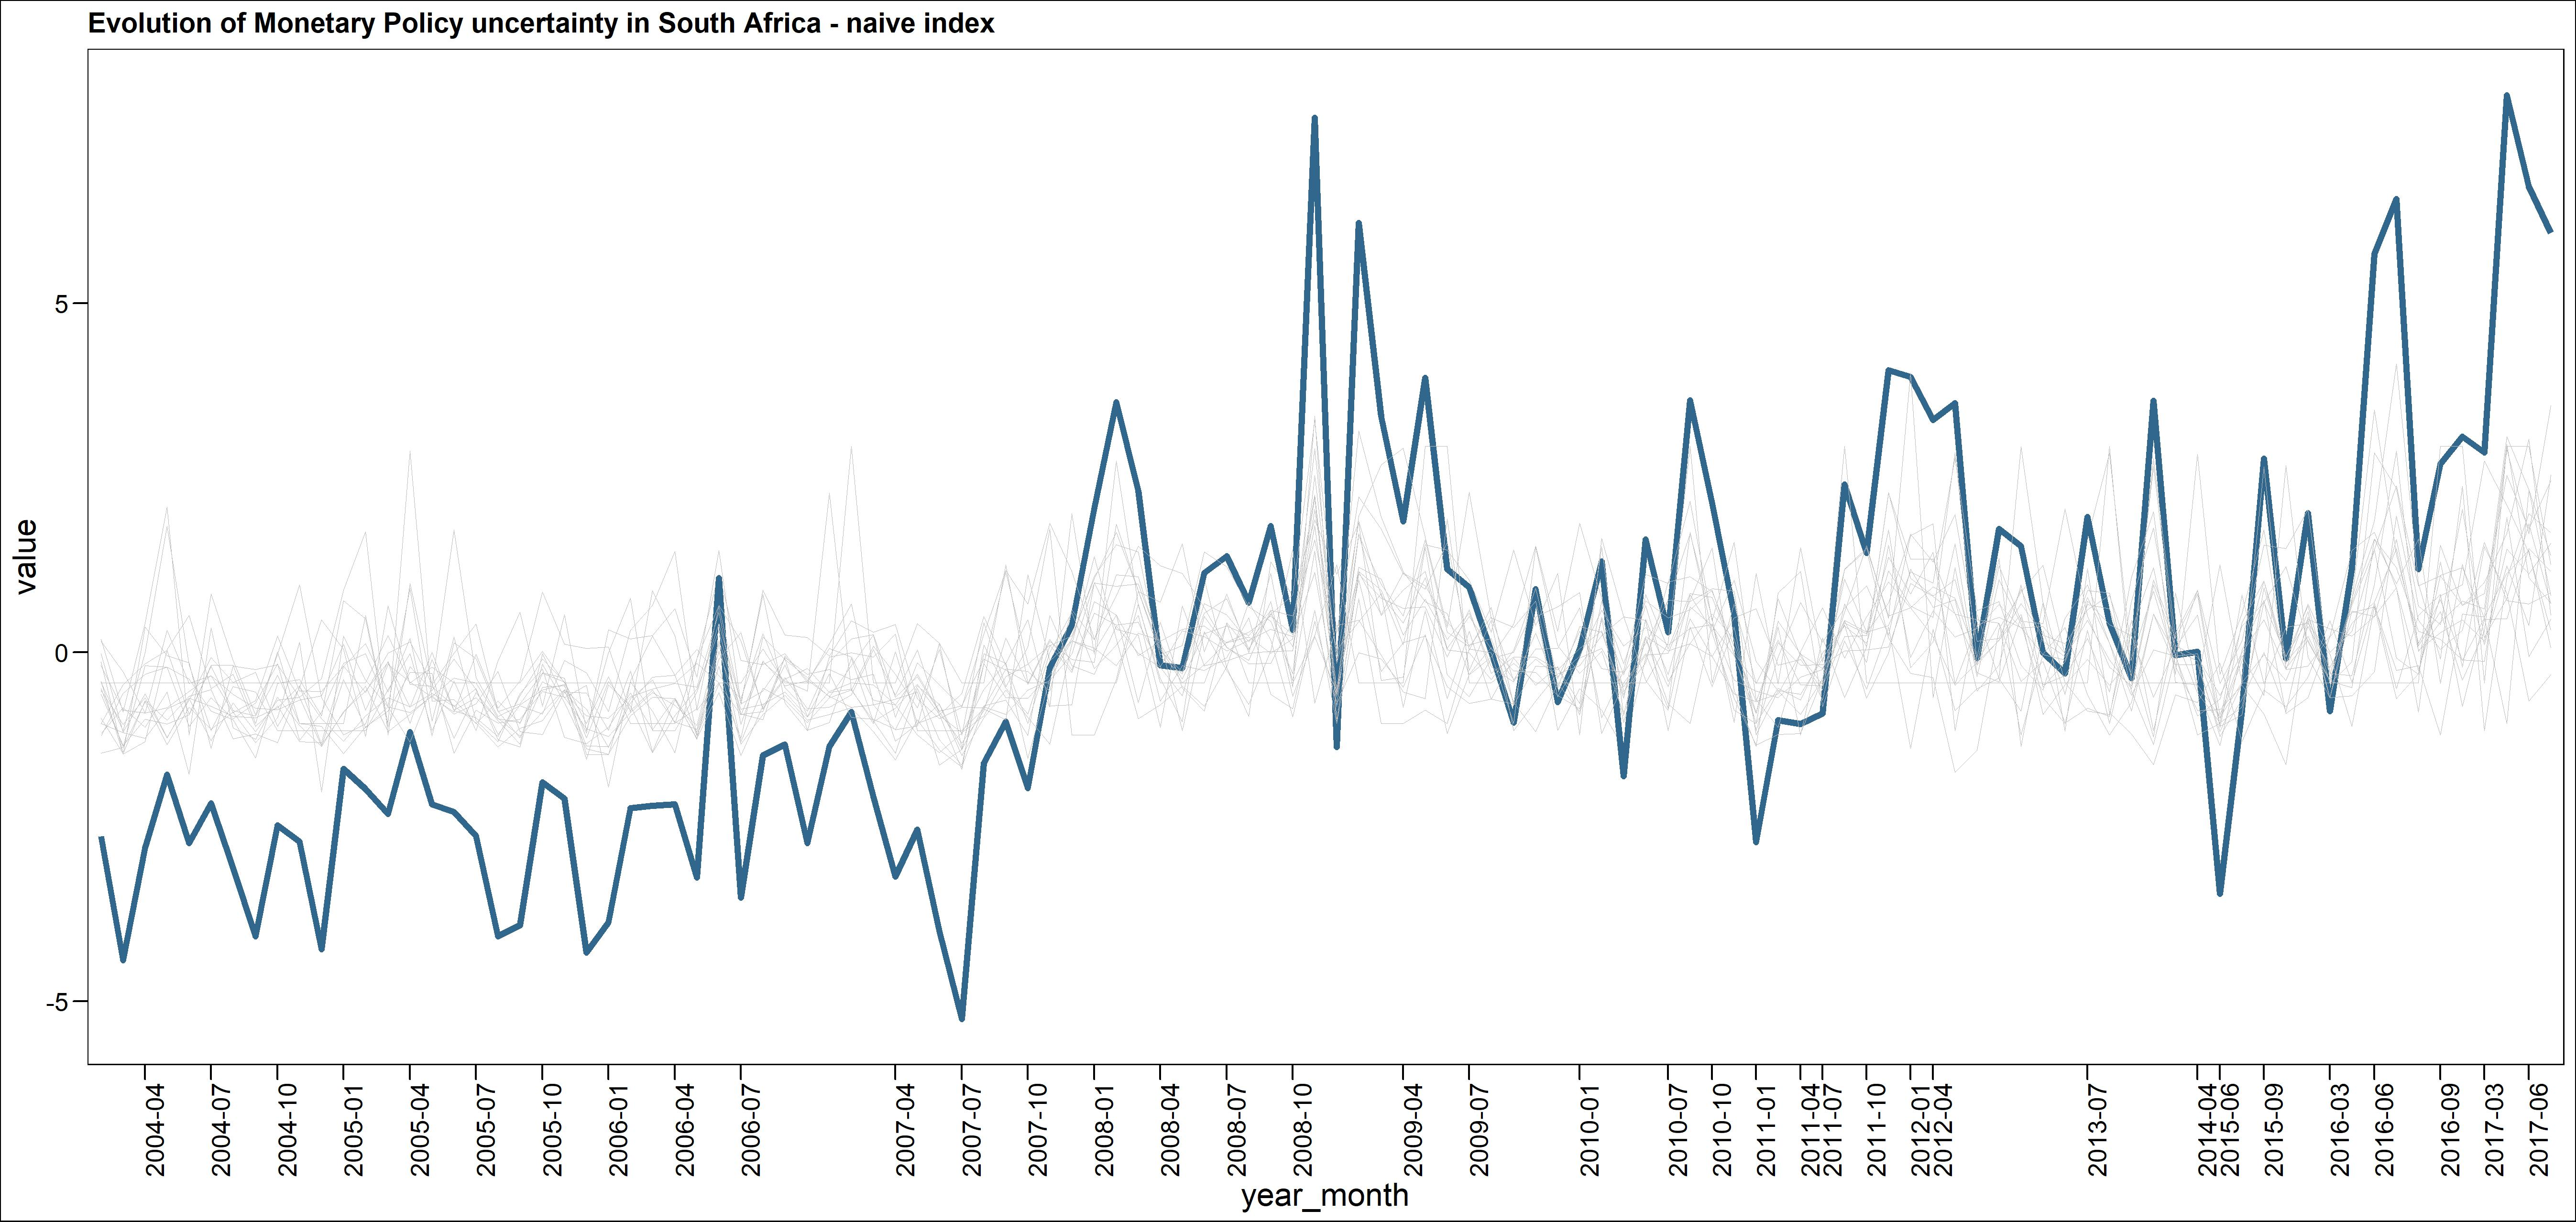
\includegraphics[width=\linewidth, keepaspectratio]{bin/monetary_comp_naive}\\
	\caption{Composite Monetary Policy uncertainty naive index. \label{fig_mon_comp_n}}
\end{figure}

\begin{figure}
	\centering
	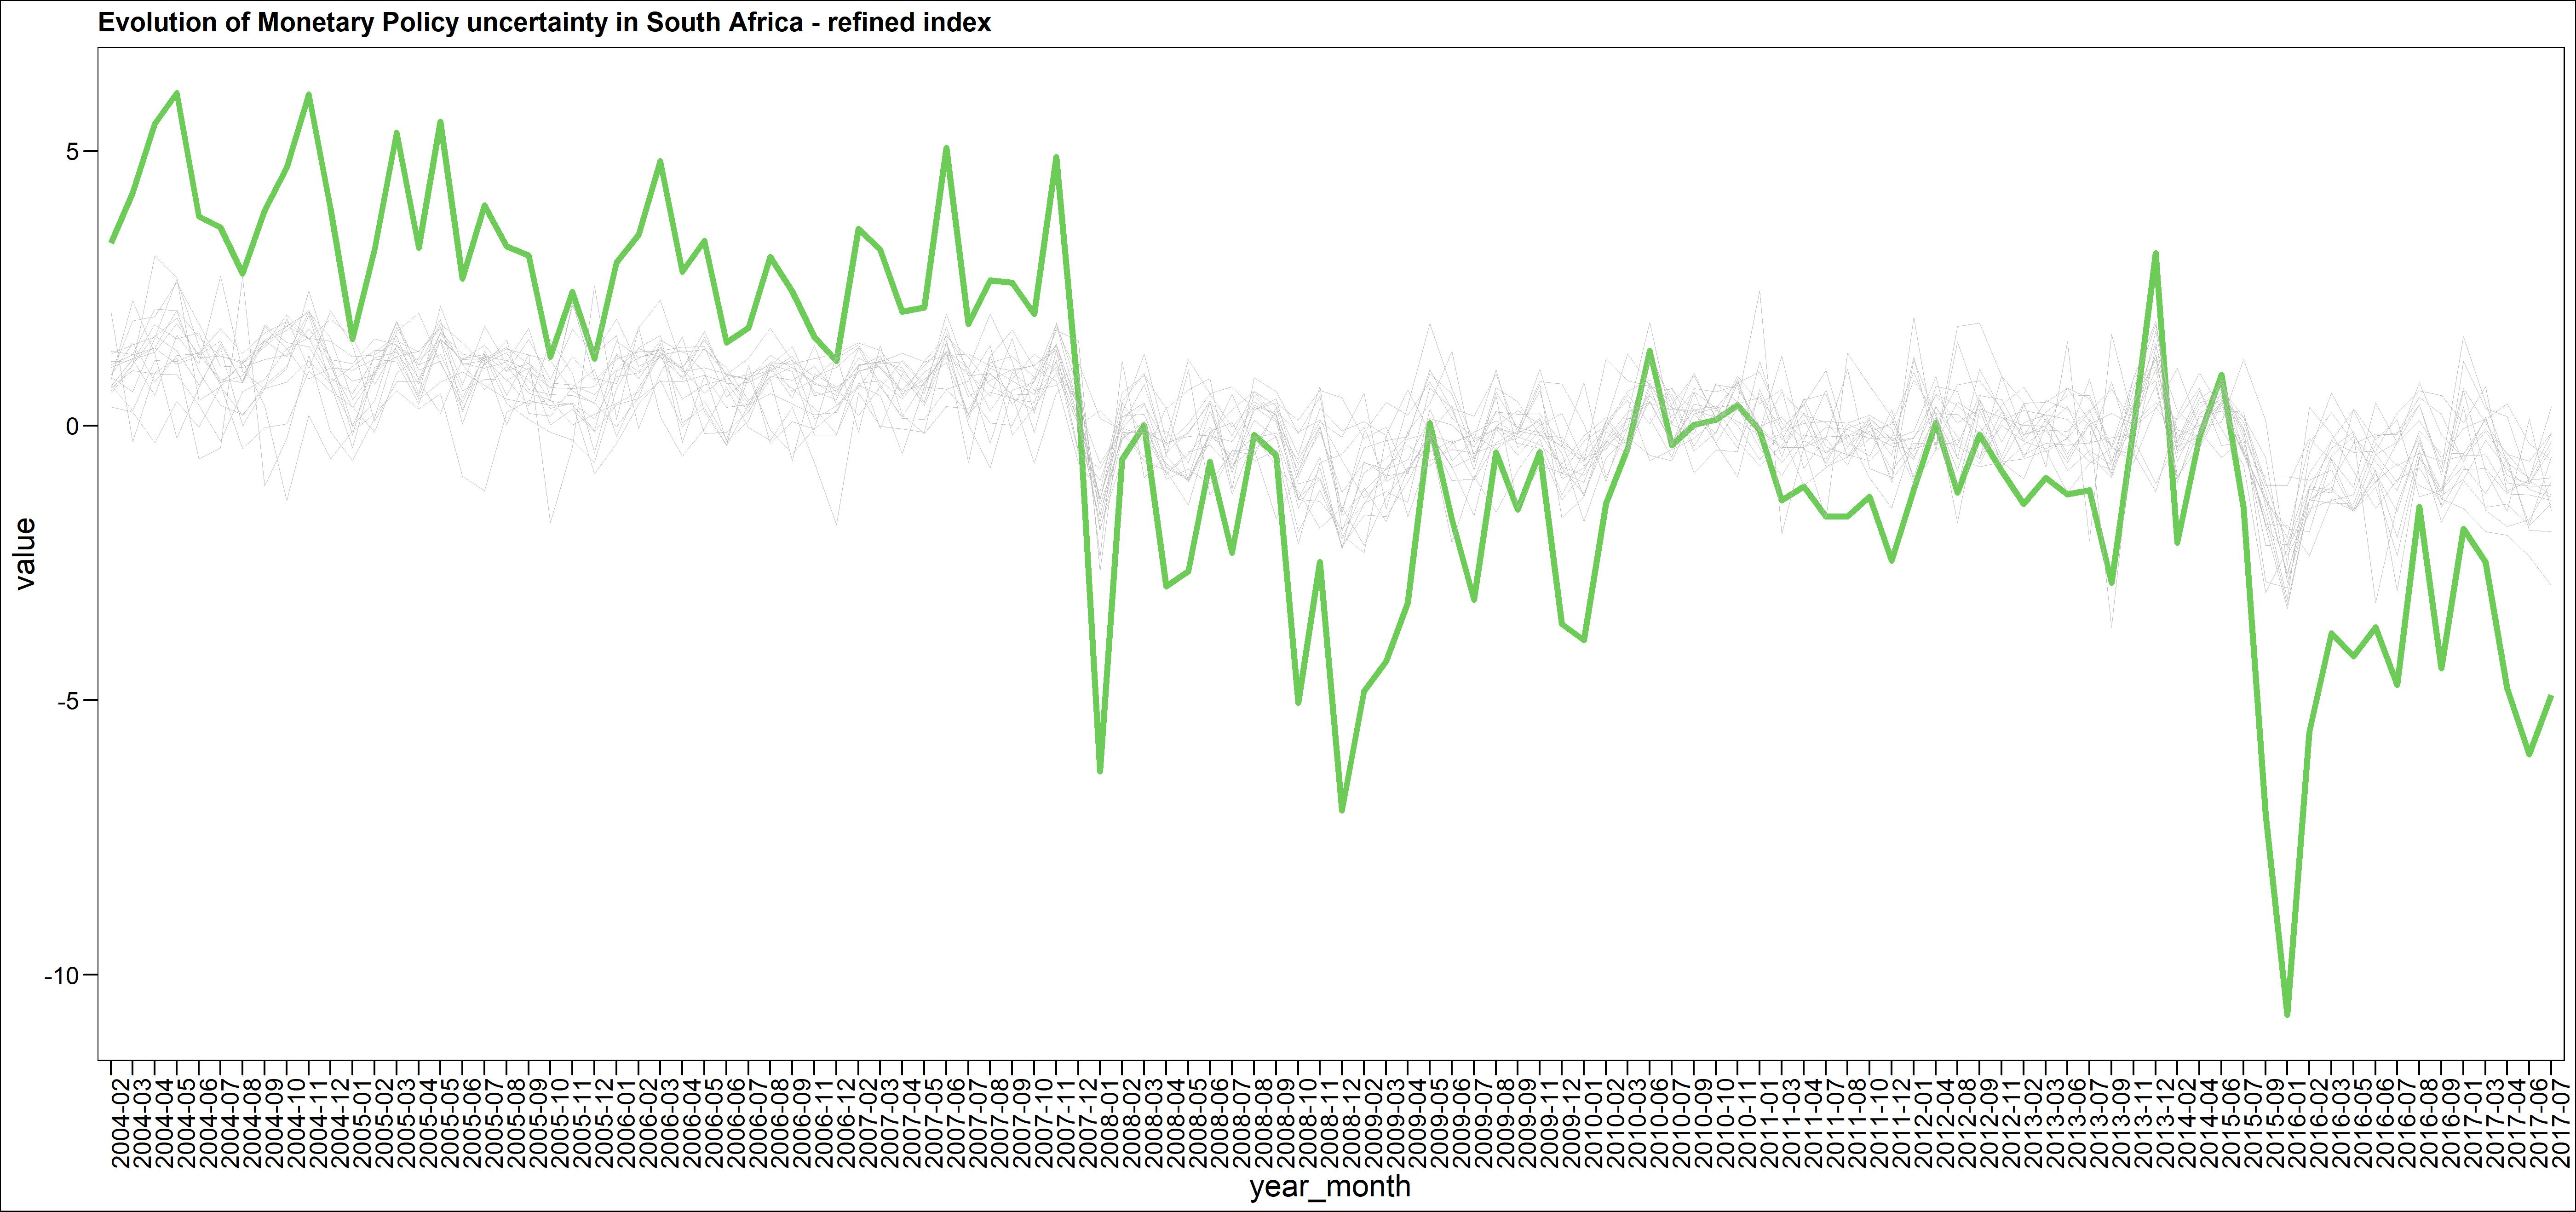
\includegraphics[width=\linewidth, keepaspectratio]{bin/monetary_comp_refine}\\
	\caption{Composite Monetary Policy uncertainty refined index. \label{fig_mon_comp_r}}
\end{figure}

\begin{figure}
	\centering
	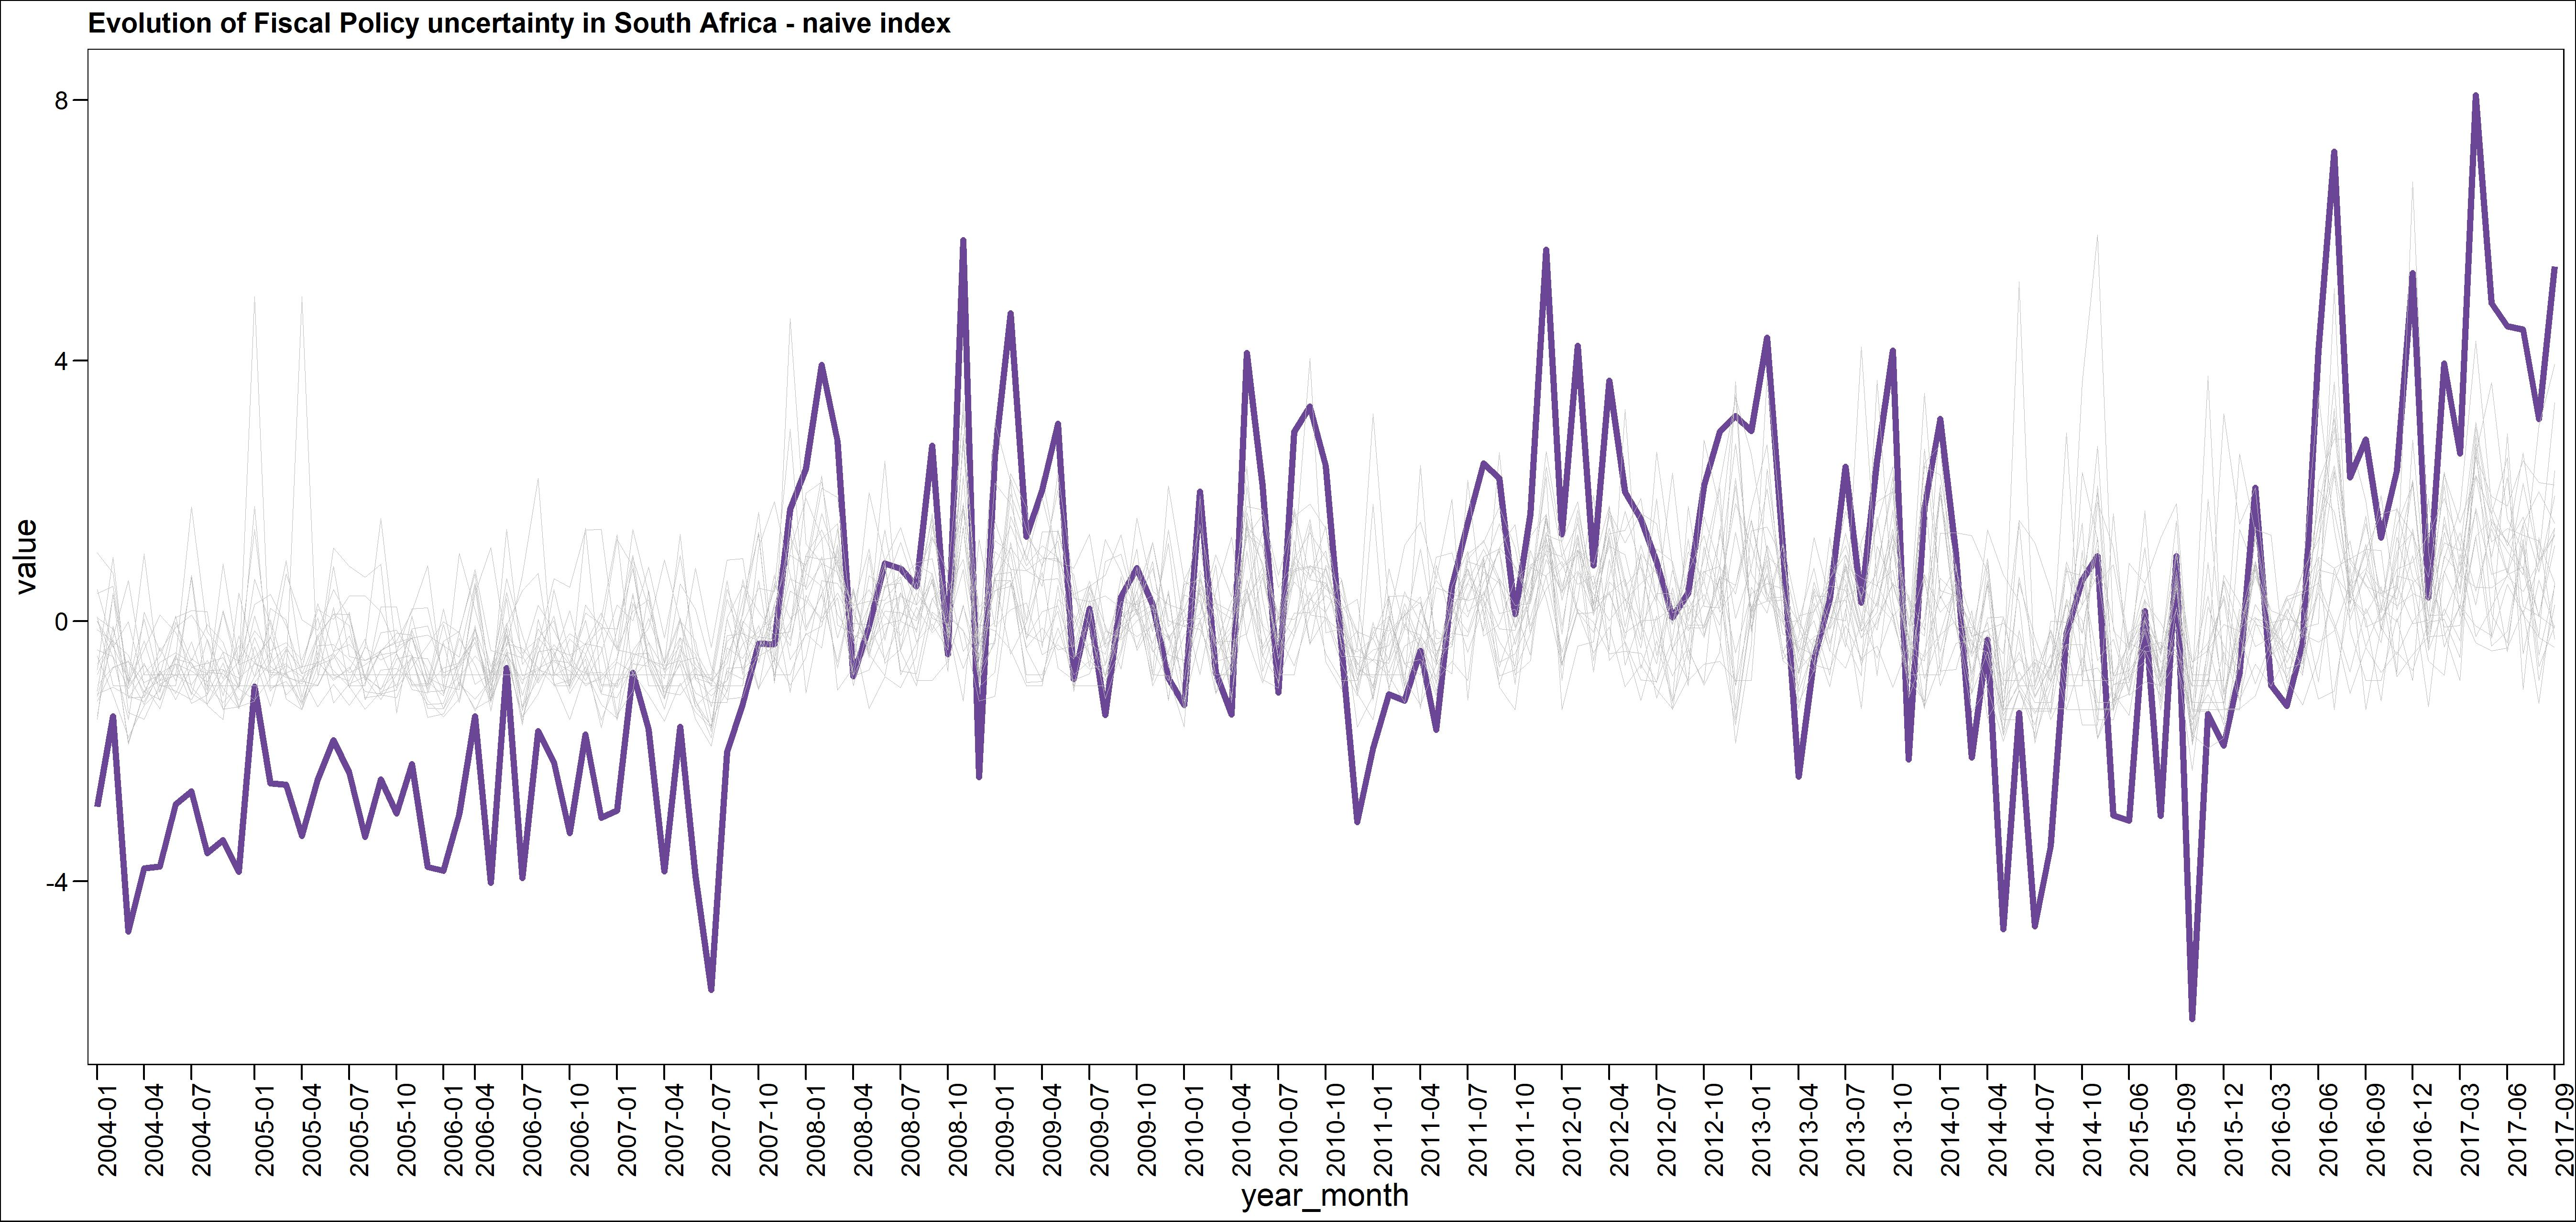
\includegraphics[width=\linewidth, keepaspectratio]{bin/fiscal_comp_naive}\\
	\caption{Composite Fiscal Policy uncertainty naive index. \label{fig_fis_comp_n}}
\end{figure}

\begin{figure}
	\centering
	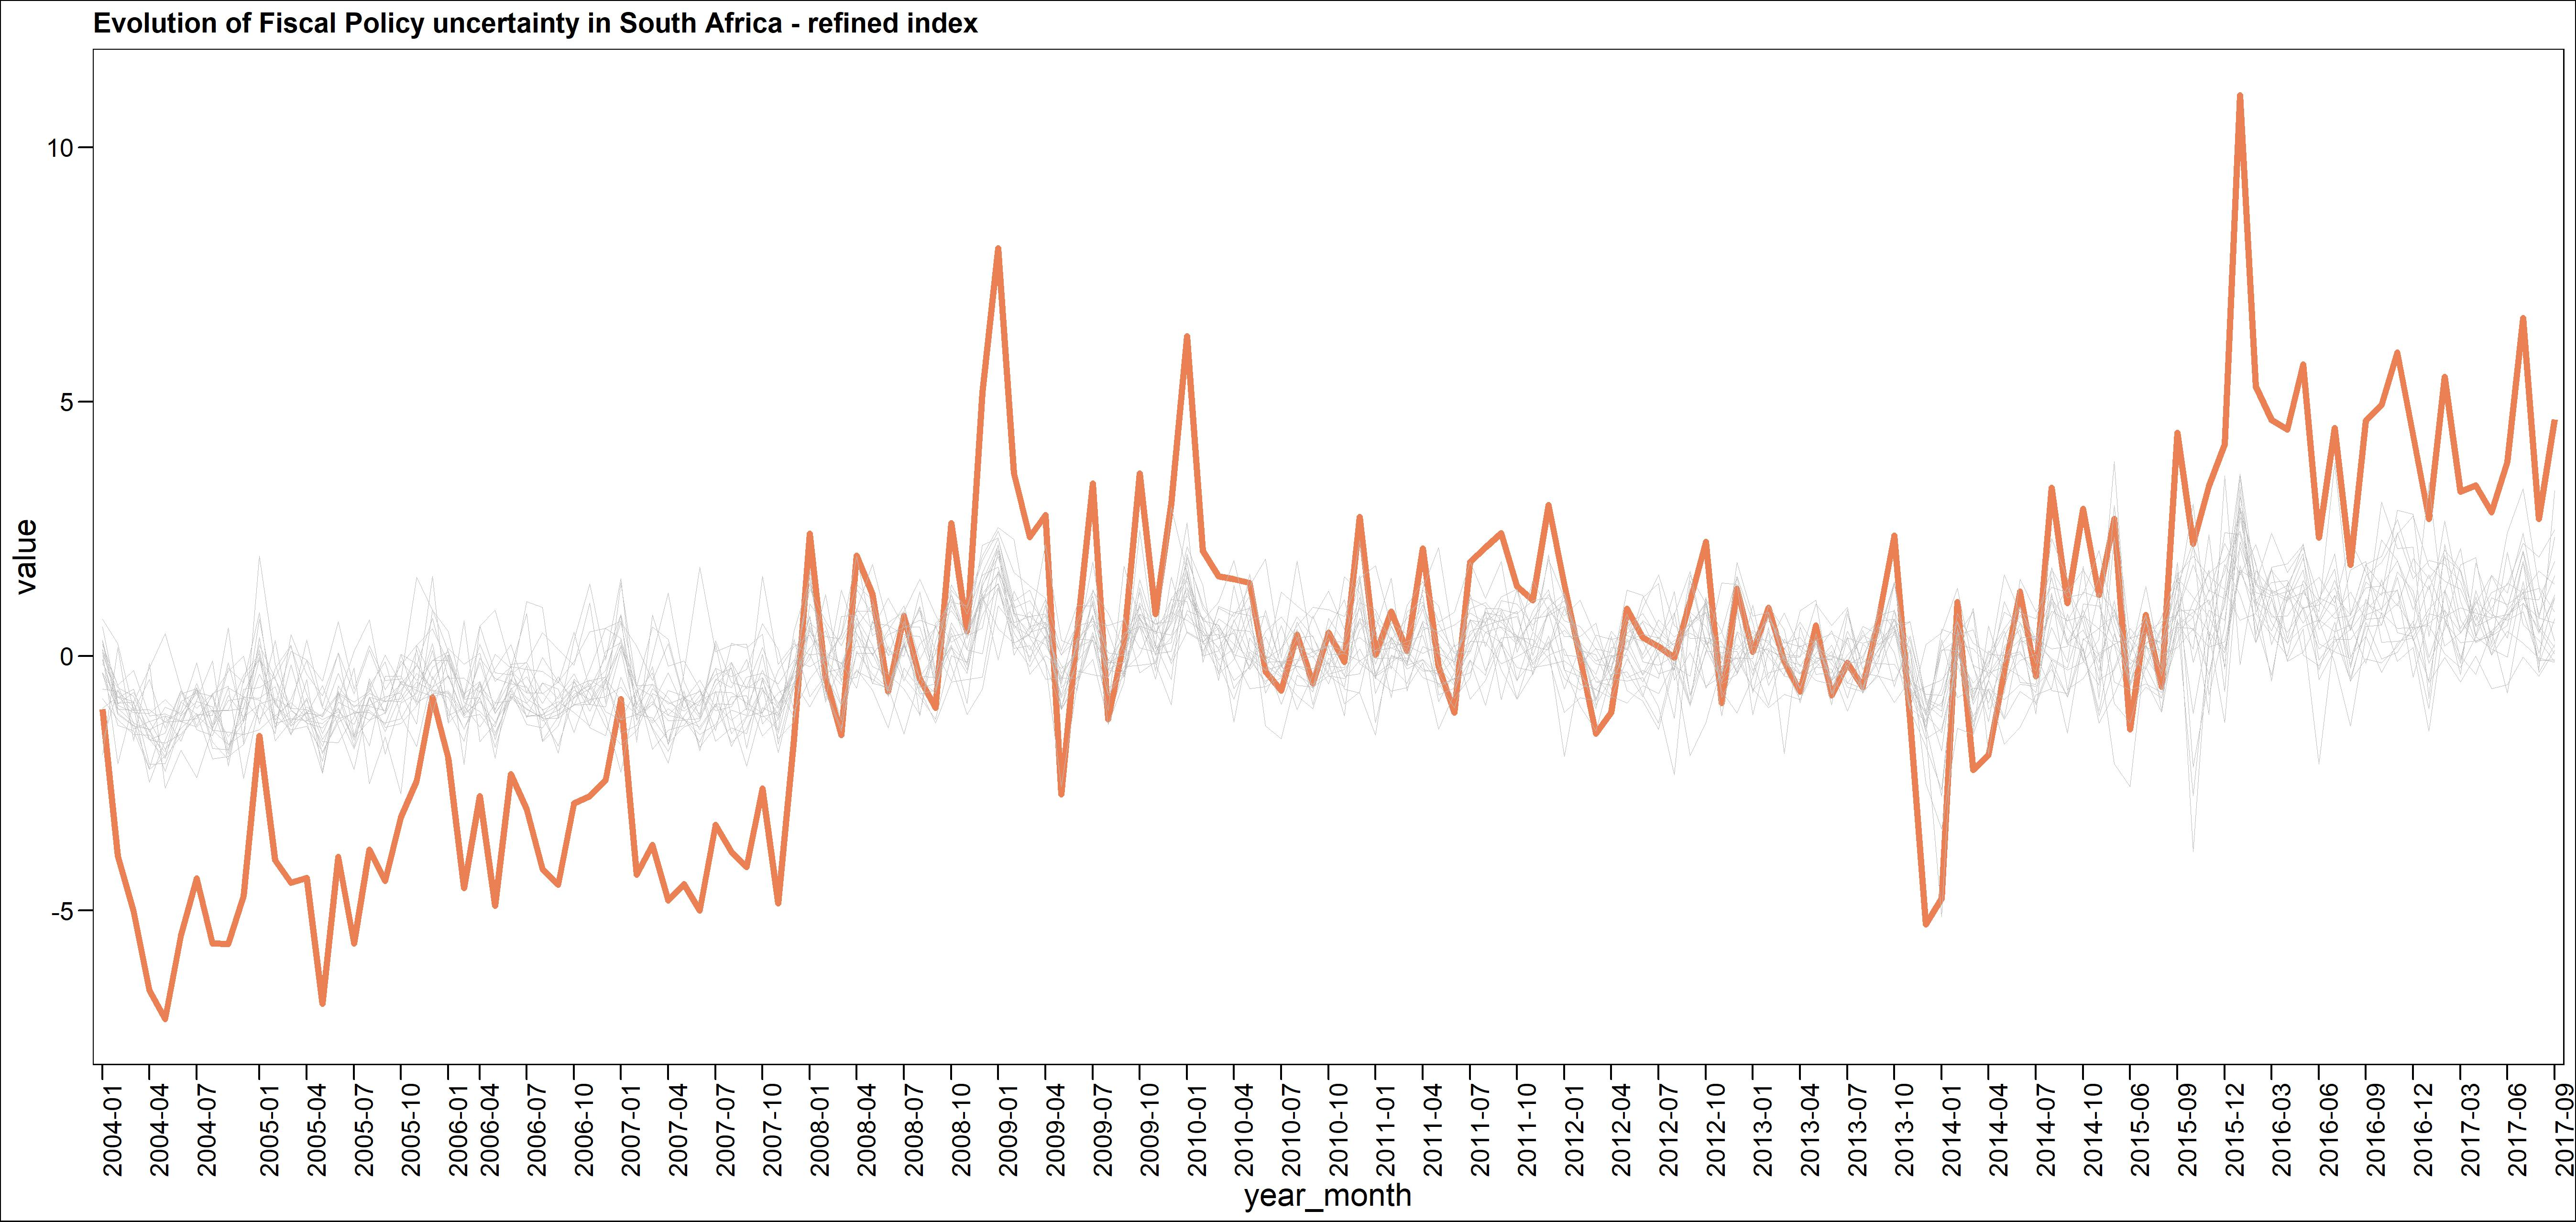
\includegraphics[width=\linewidth, keepaspectratio]{bin/fiscal_comp_refine}\\	
	\caption{Composite Fiscal Policy uncertainty refined index. \label{fig_fis_comp_r}}
\end{figure}

\begin{figure}
	\centering
	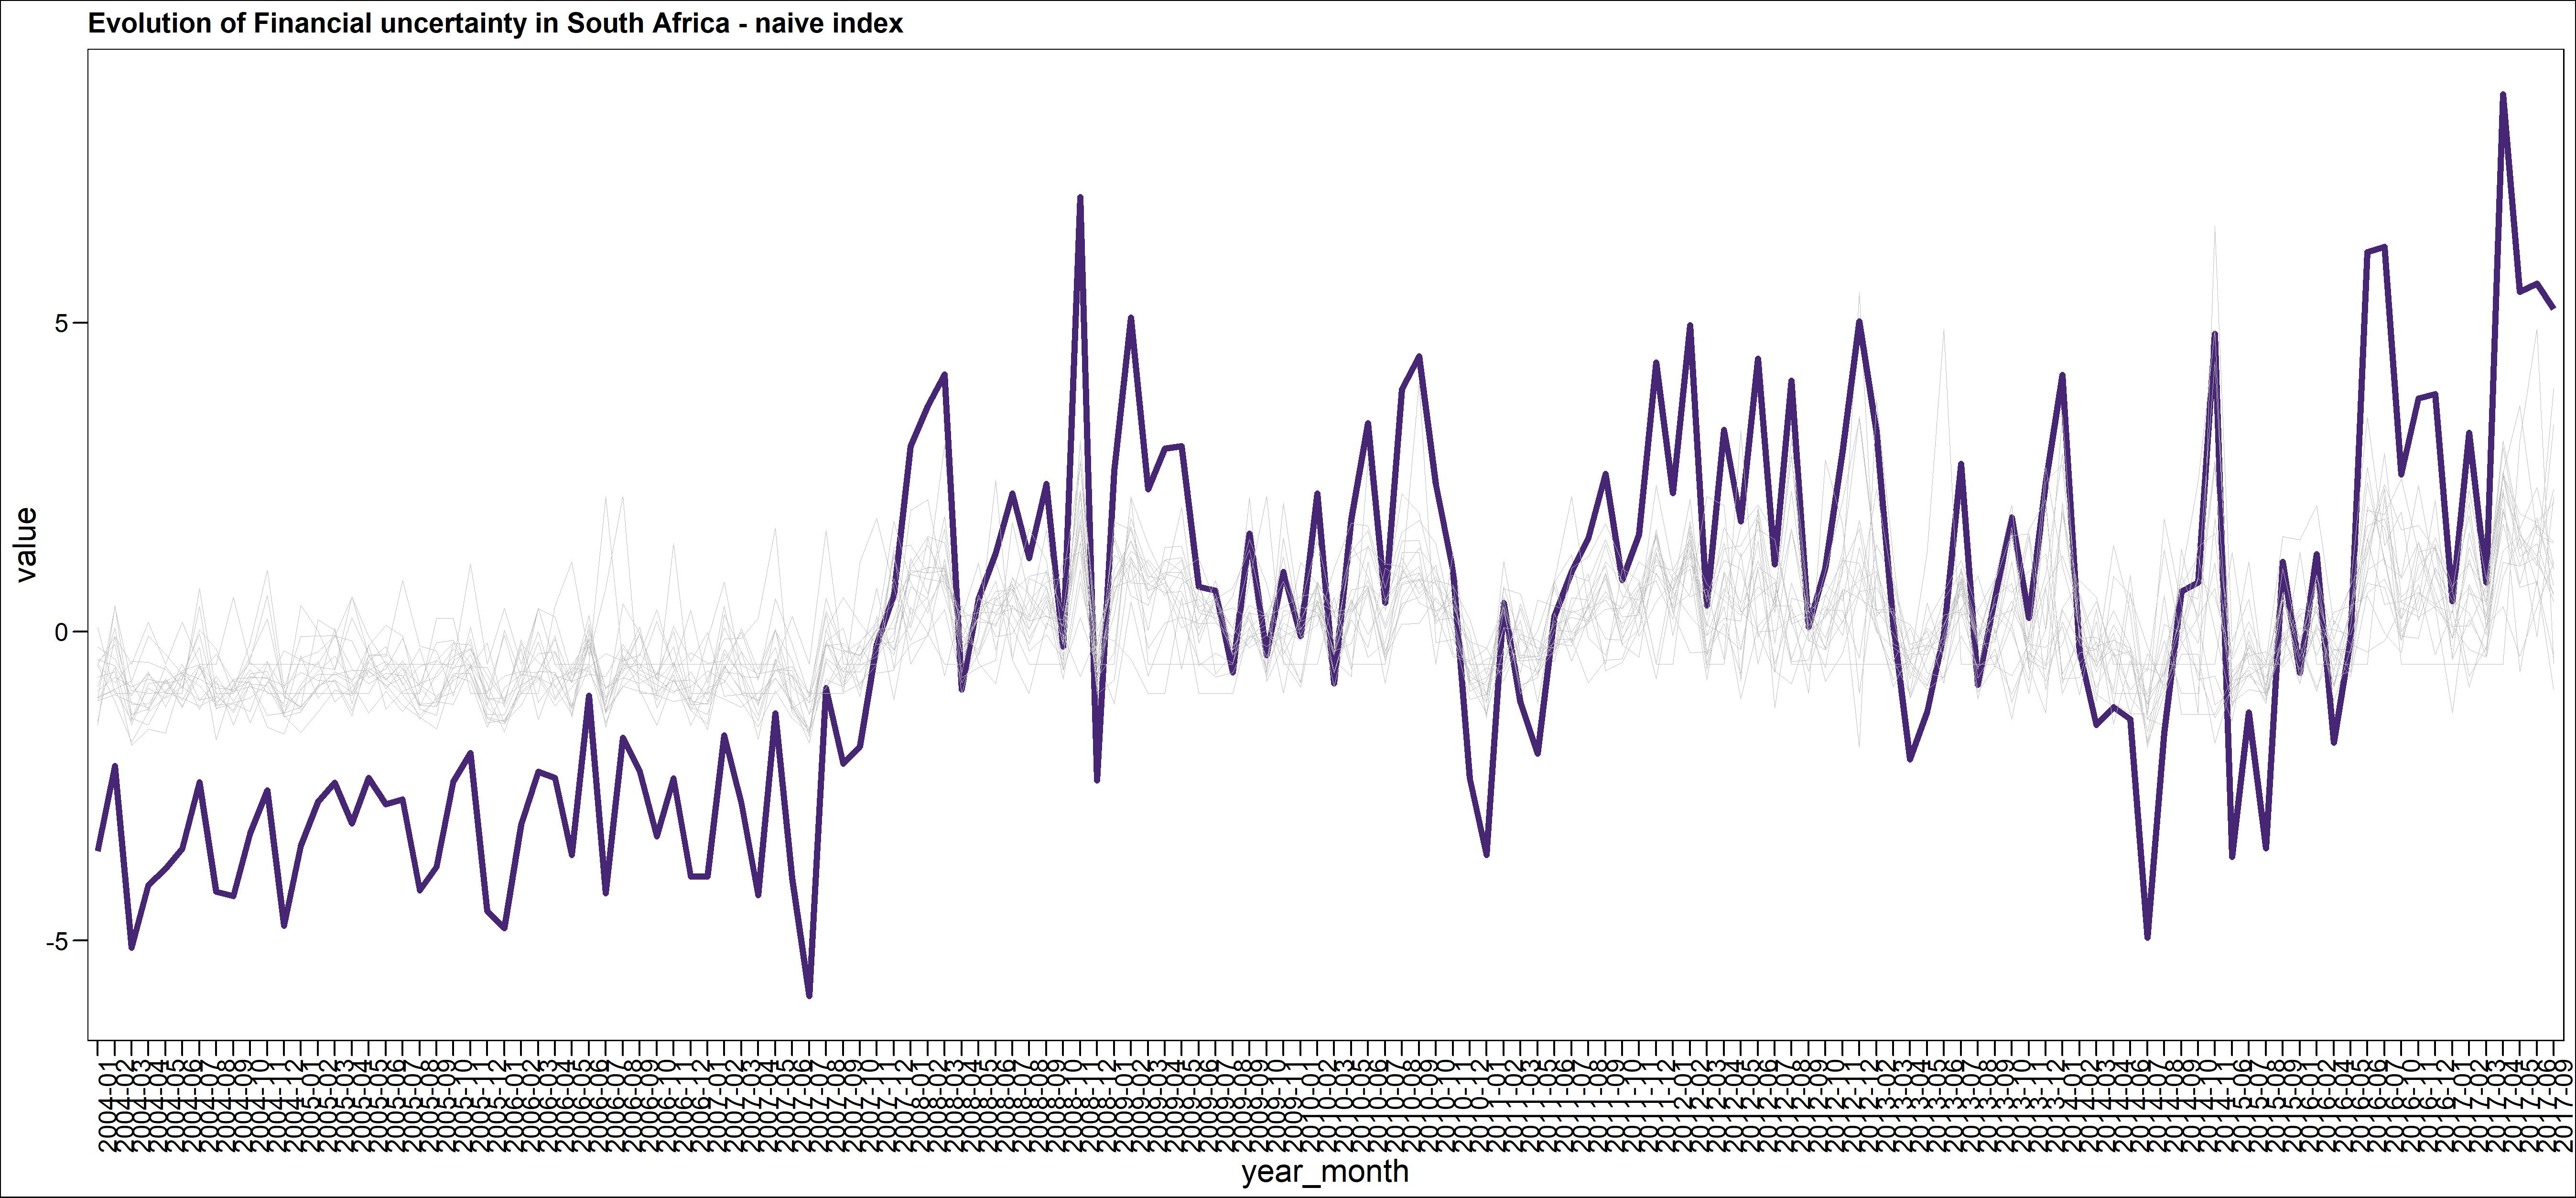
\includegraphics[width=\linewidth, keepaspectratio]{bin/financial_comp_naive}\\
	\caption{Composite Financial market uncertainty naive index. \label{fig_fin_comp_n}}
\end{figure}

\begin{figure}
	\centering
	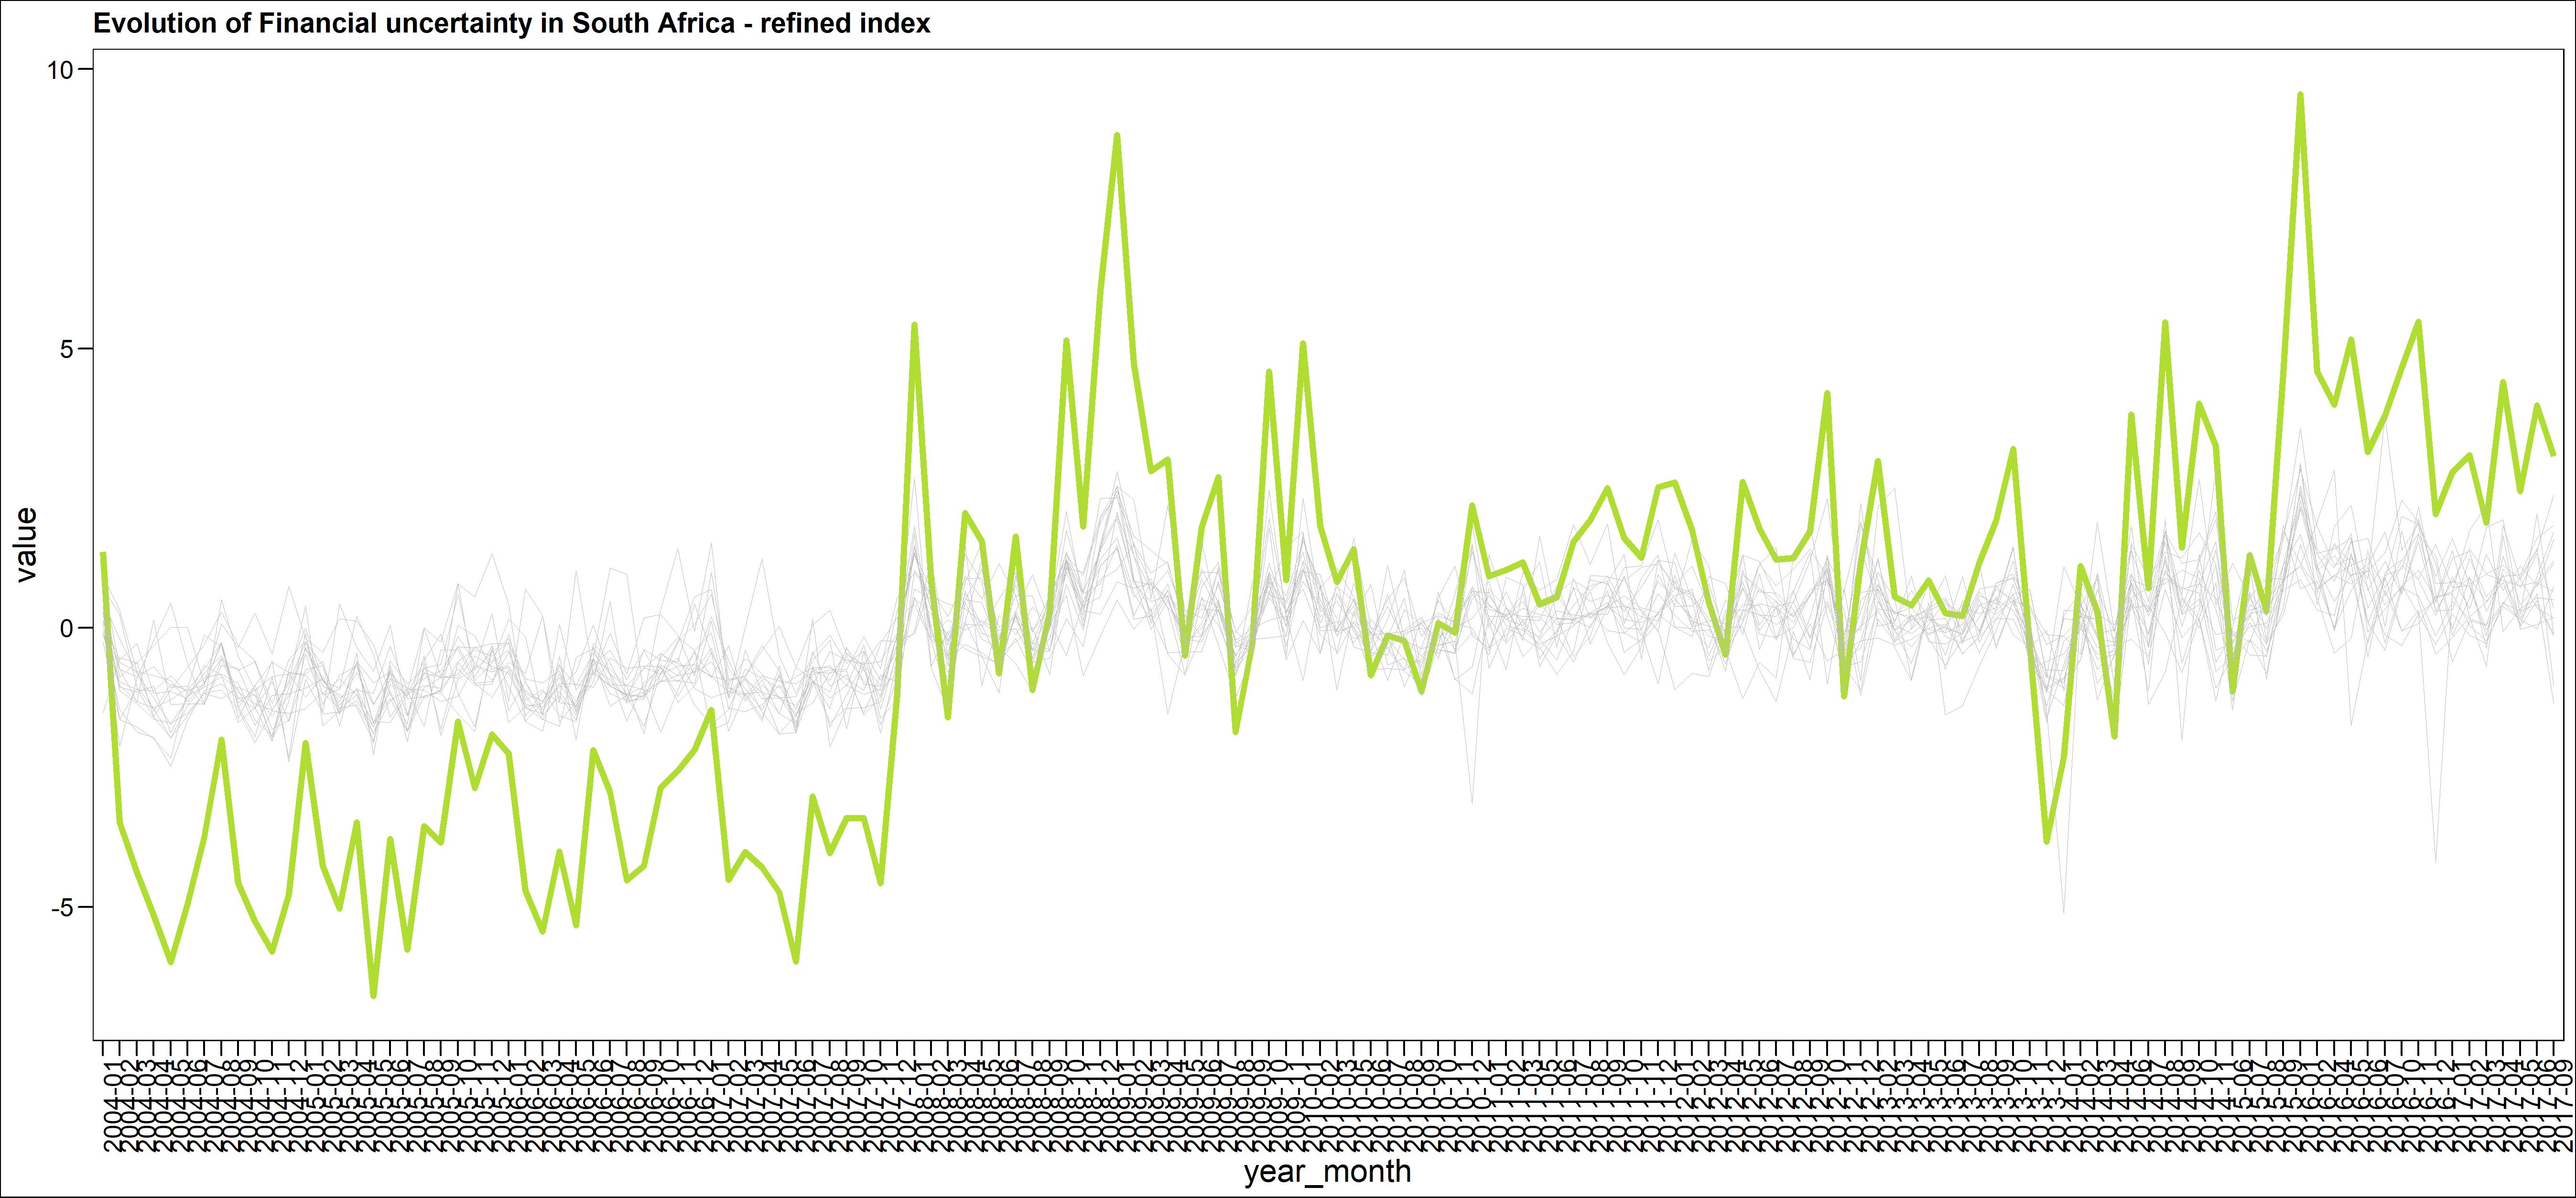
\includegraphics[width=\linewidth, keepaspectratio]{bin/financial_comp_refine}\\
	\caption{Composite Financial market uncertainty refined index. \label{fig_fin_comp_r}}
\end{figure}

\begin{figure}
	\centering
	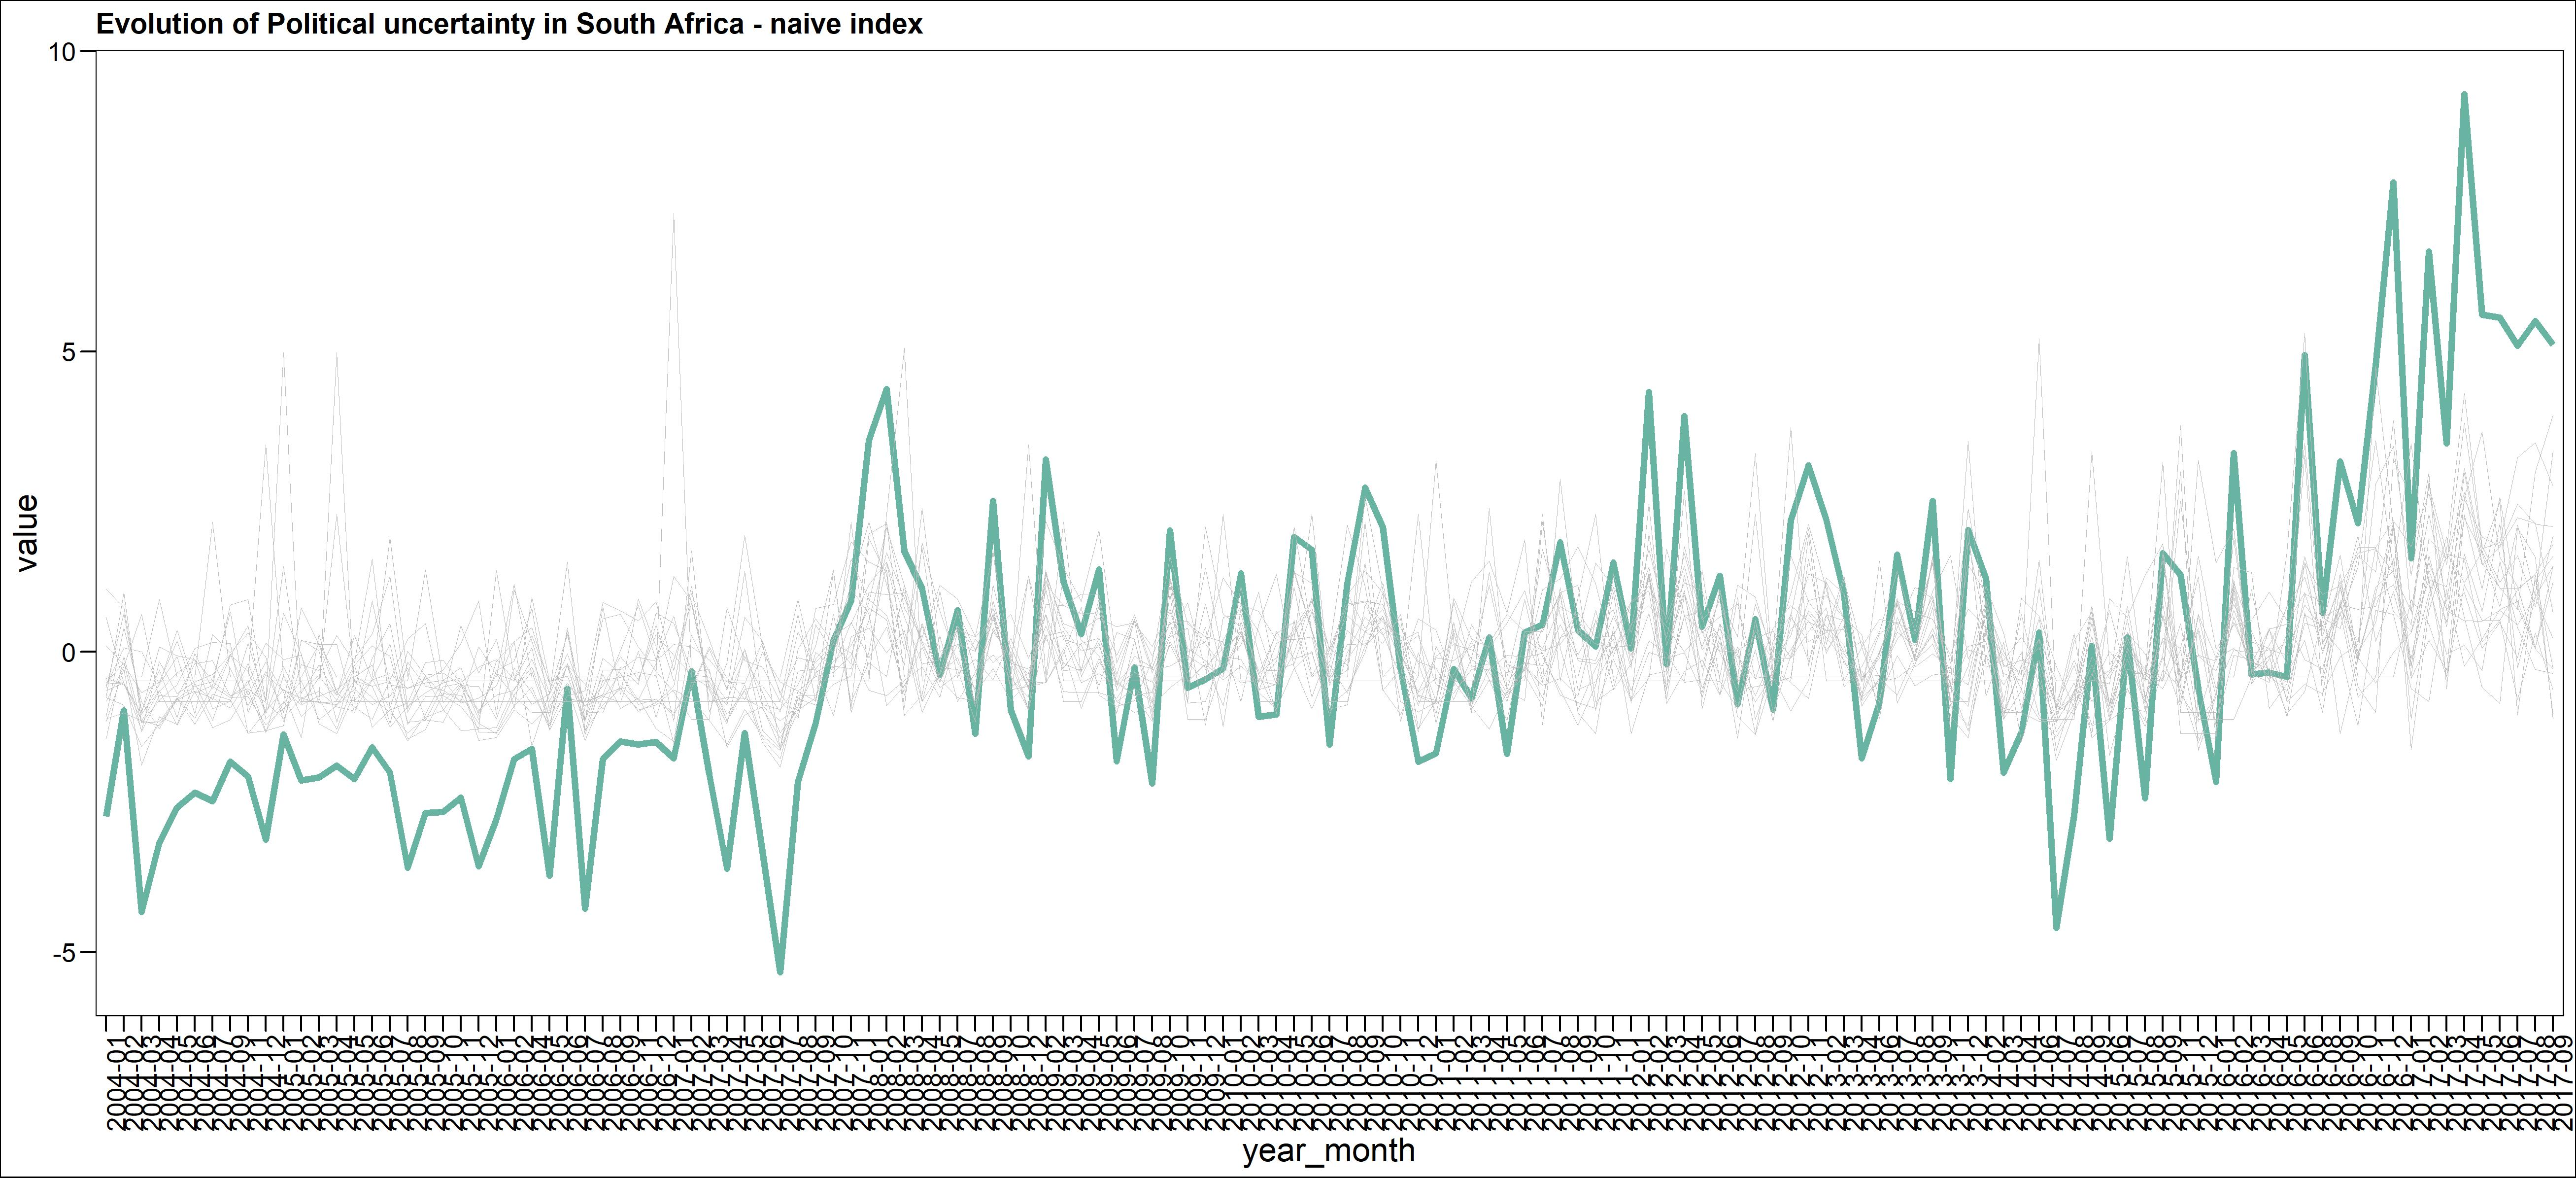
\includegraphics[width=\linewidth, keepaspectratio]{bin/pol_comp_naive}\\
	\caption{Composite Political uncertainty naive index. \label{fig_pol_comp_n}}
\end{figure}

\begin{figure}
	\centering
	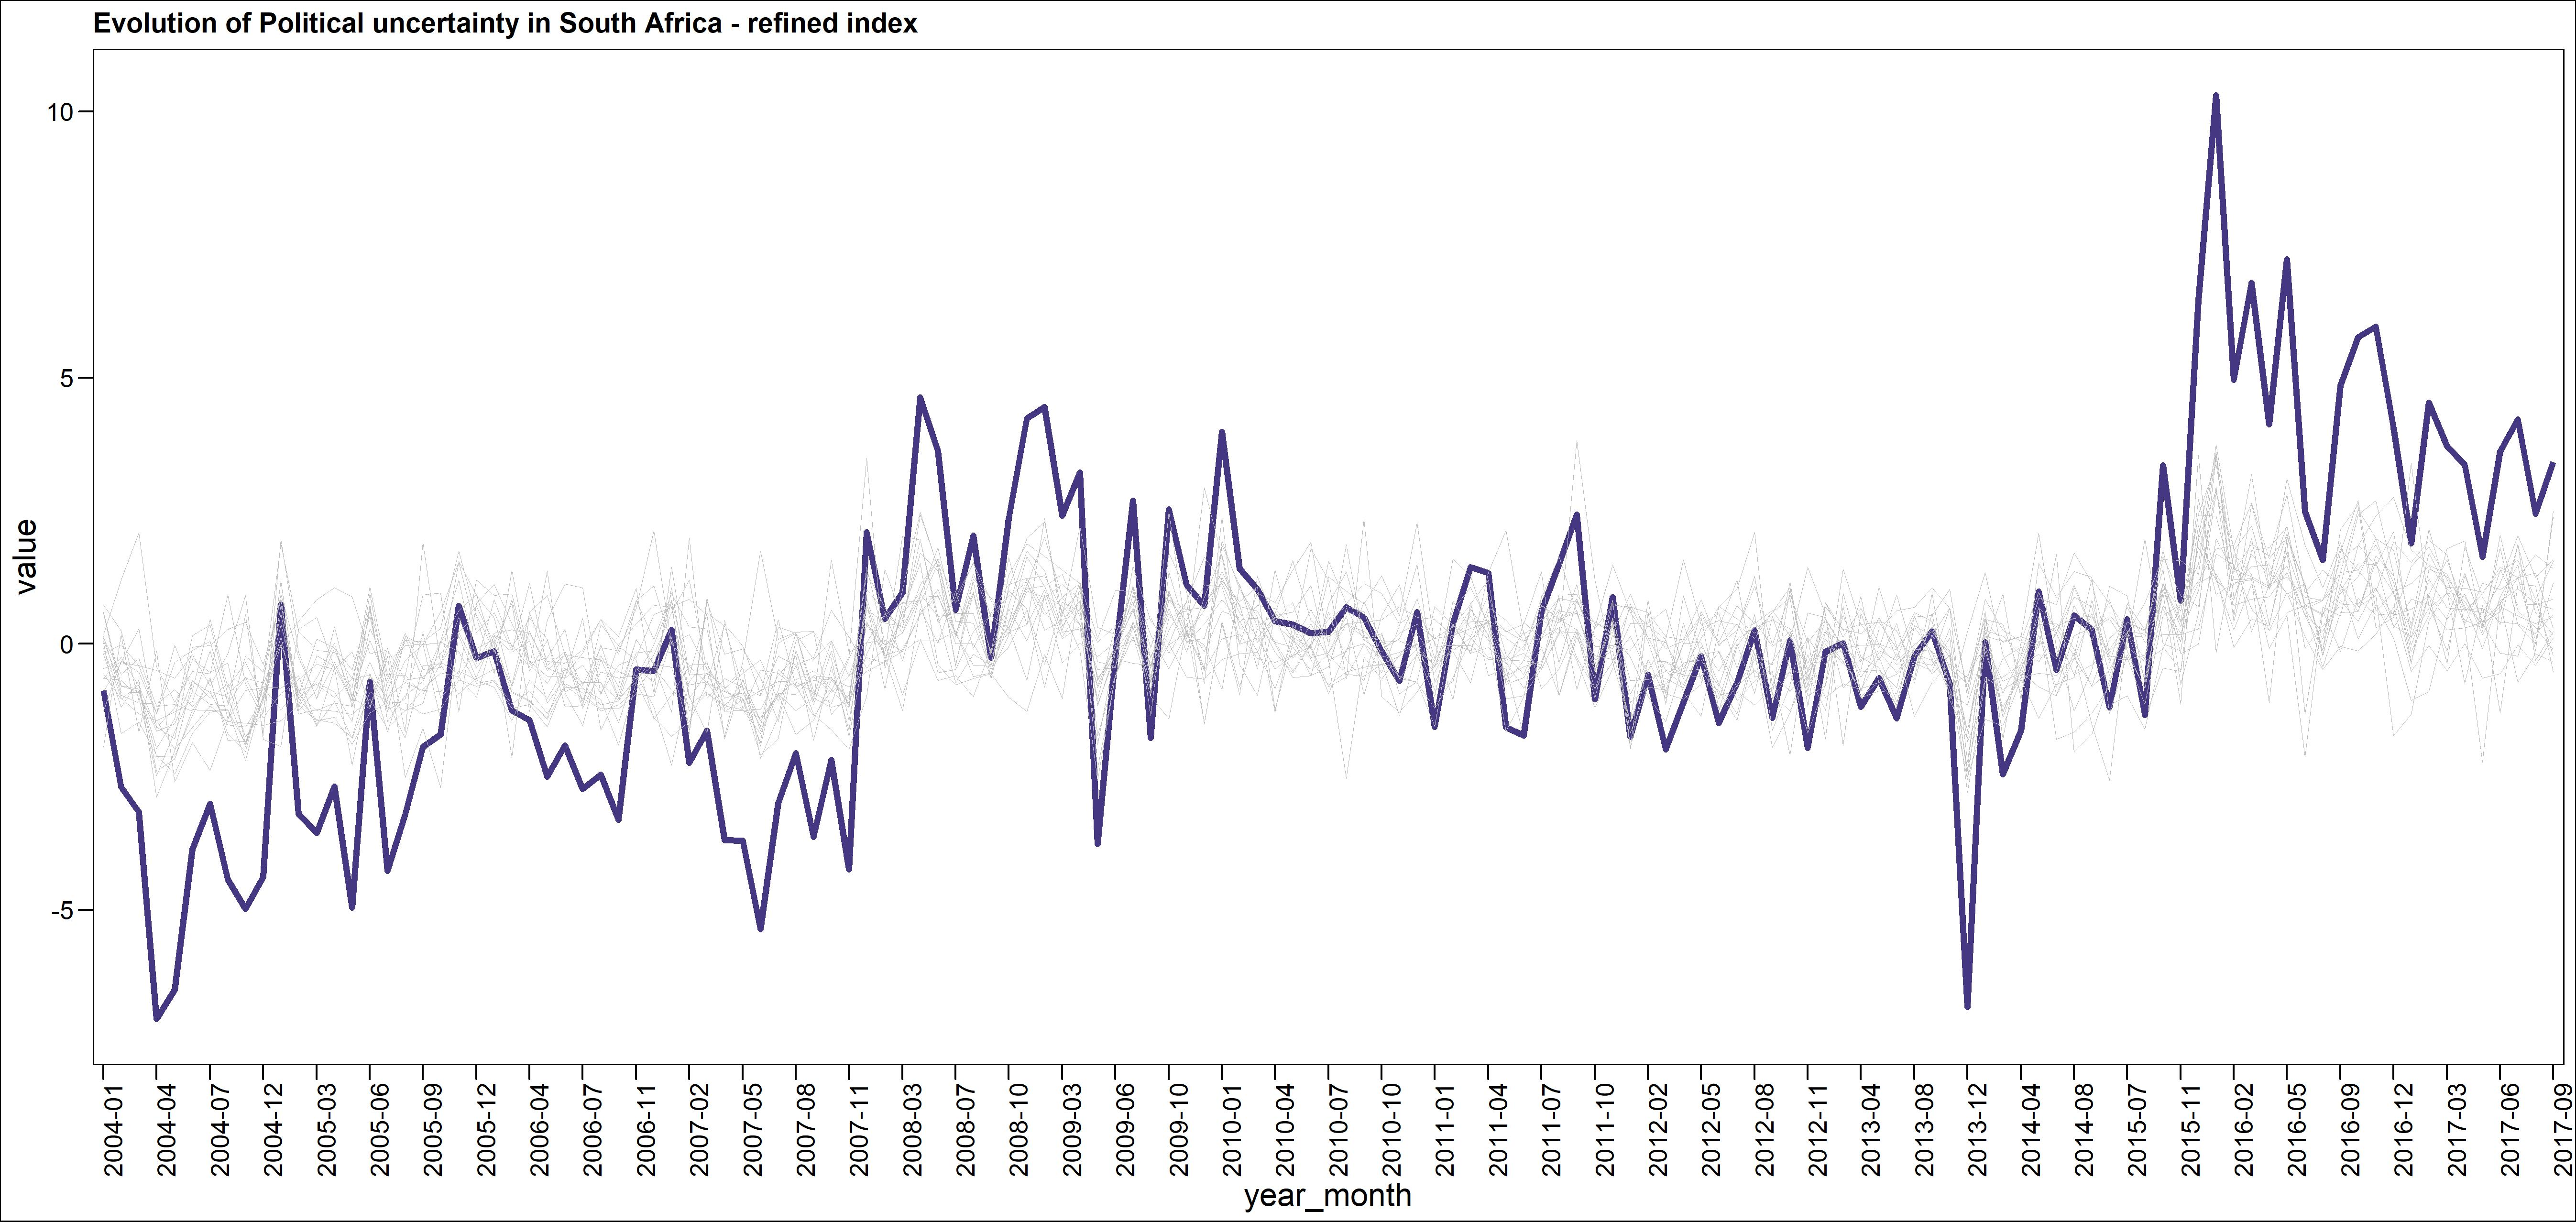
\includegraphics[width=\linewidth, keepaspectratio]{bin/pol_comp_refine}\\
	\caption{Composite Political uncertainty refined index. \label{fig_pol_comp_r}}
\end{figure}

\section{\texorpdfstring{The evolution of Economic Policy Uncertainty in
South Africa
\label{sec_discuss}}{The evolution of Economic Policy Uncertainty in South Africa }}\label{the-evolution-of-economic-policy-uncertainty-in-south-africa}

Observing figures \ref{mon_comp_final} to \ref{pol_comp_final} showing
the composite naive index in grey and the refined index in colour,
highlights the similarities in the results. The main difference between
the indices is that the refined index is, as the name suggests, more
refined. In all cases, the refined index is less volatile than its naive
counterpart and shocks are less persistent. For this reason, the
remainder of this paper works solely with the refined composite index.

Figures \ref{mon_comp_final} to \ref{pol_comp_final} also show the
similarity in peak periods across the four topics. To test this
formally, a structural break test was performed on each composite index
to identify whether significant shifts in uncertainty is common across
topics\footnote{The calculations show breakpoints for the political
  uncertainty index at November 2007, February 2010 and August 2015. For
  the fiscal policy uncertainty index at December 2007, January 2012 and
  August 2015. For the monetary policy uncertainty index at November
  2007 and April 2014. For the financial uncertainty index at December
  2007 and July 2014.}. From these results, two distinct periods are
identified (highlighted panels in figures \ref{mon_comp_final} to
\ref{pol_comp_final}). These respective periods are discussed below as
comprehensively as possible by first identifying the most uncertain
months in the period and then the most uncertain days\footnote{For the
  subsequent sections, numerous newspaper articles in the constructed
  dataset was consulted to build a chronological narrative of economic
  policy uncertainty in South Africa. Along with this, various internet
  sources was consulted to identify the largest news stories, including:
  South African History Online (``2016 in Review''
  \protect\hyperlink{ref-2016}{2016}), BBC News (``South Africa Profile
  - Timeline'' \protect\hyperlink{ref-2018}{2018}) and Mekuto
  (\protect\hyperlink{ref-Mekuto2017}{2017}).}. Albeit that the
subsequent sections aim to provide an in-depth narrative of the events
that contributed to uncertainty during these periods, it is by no means
an exhaustive account.

\begin{figure}
	\centering
	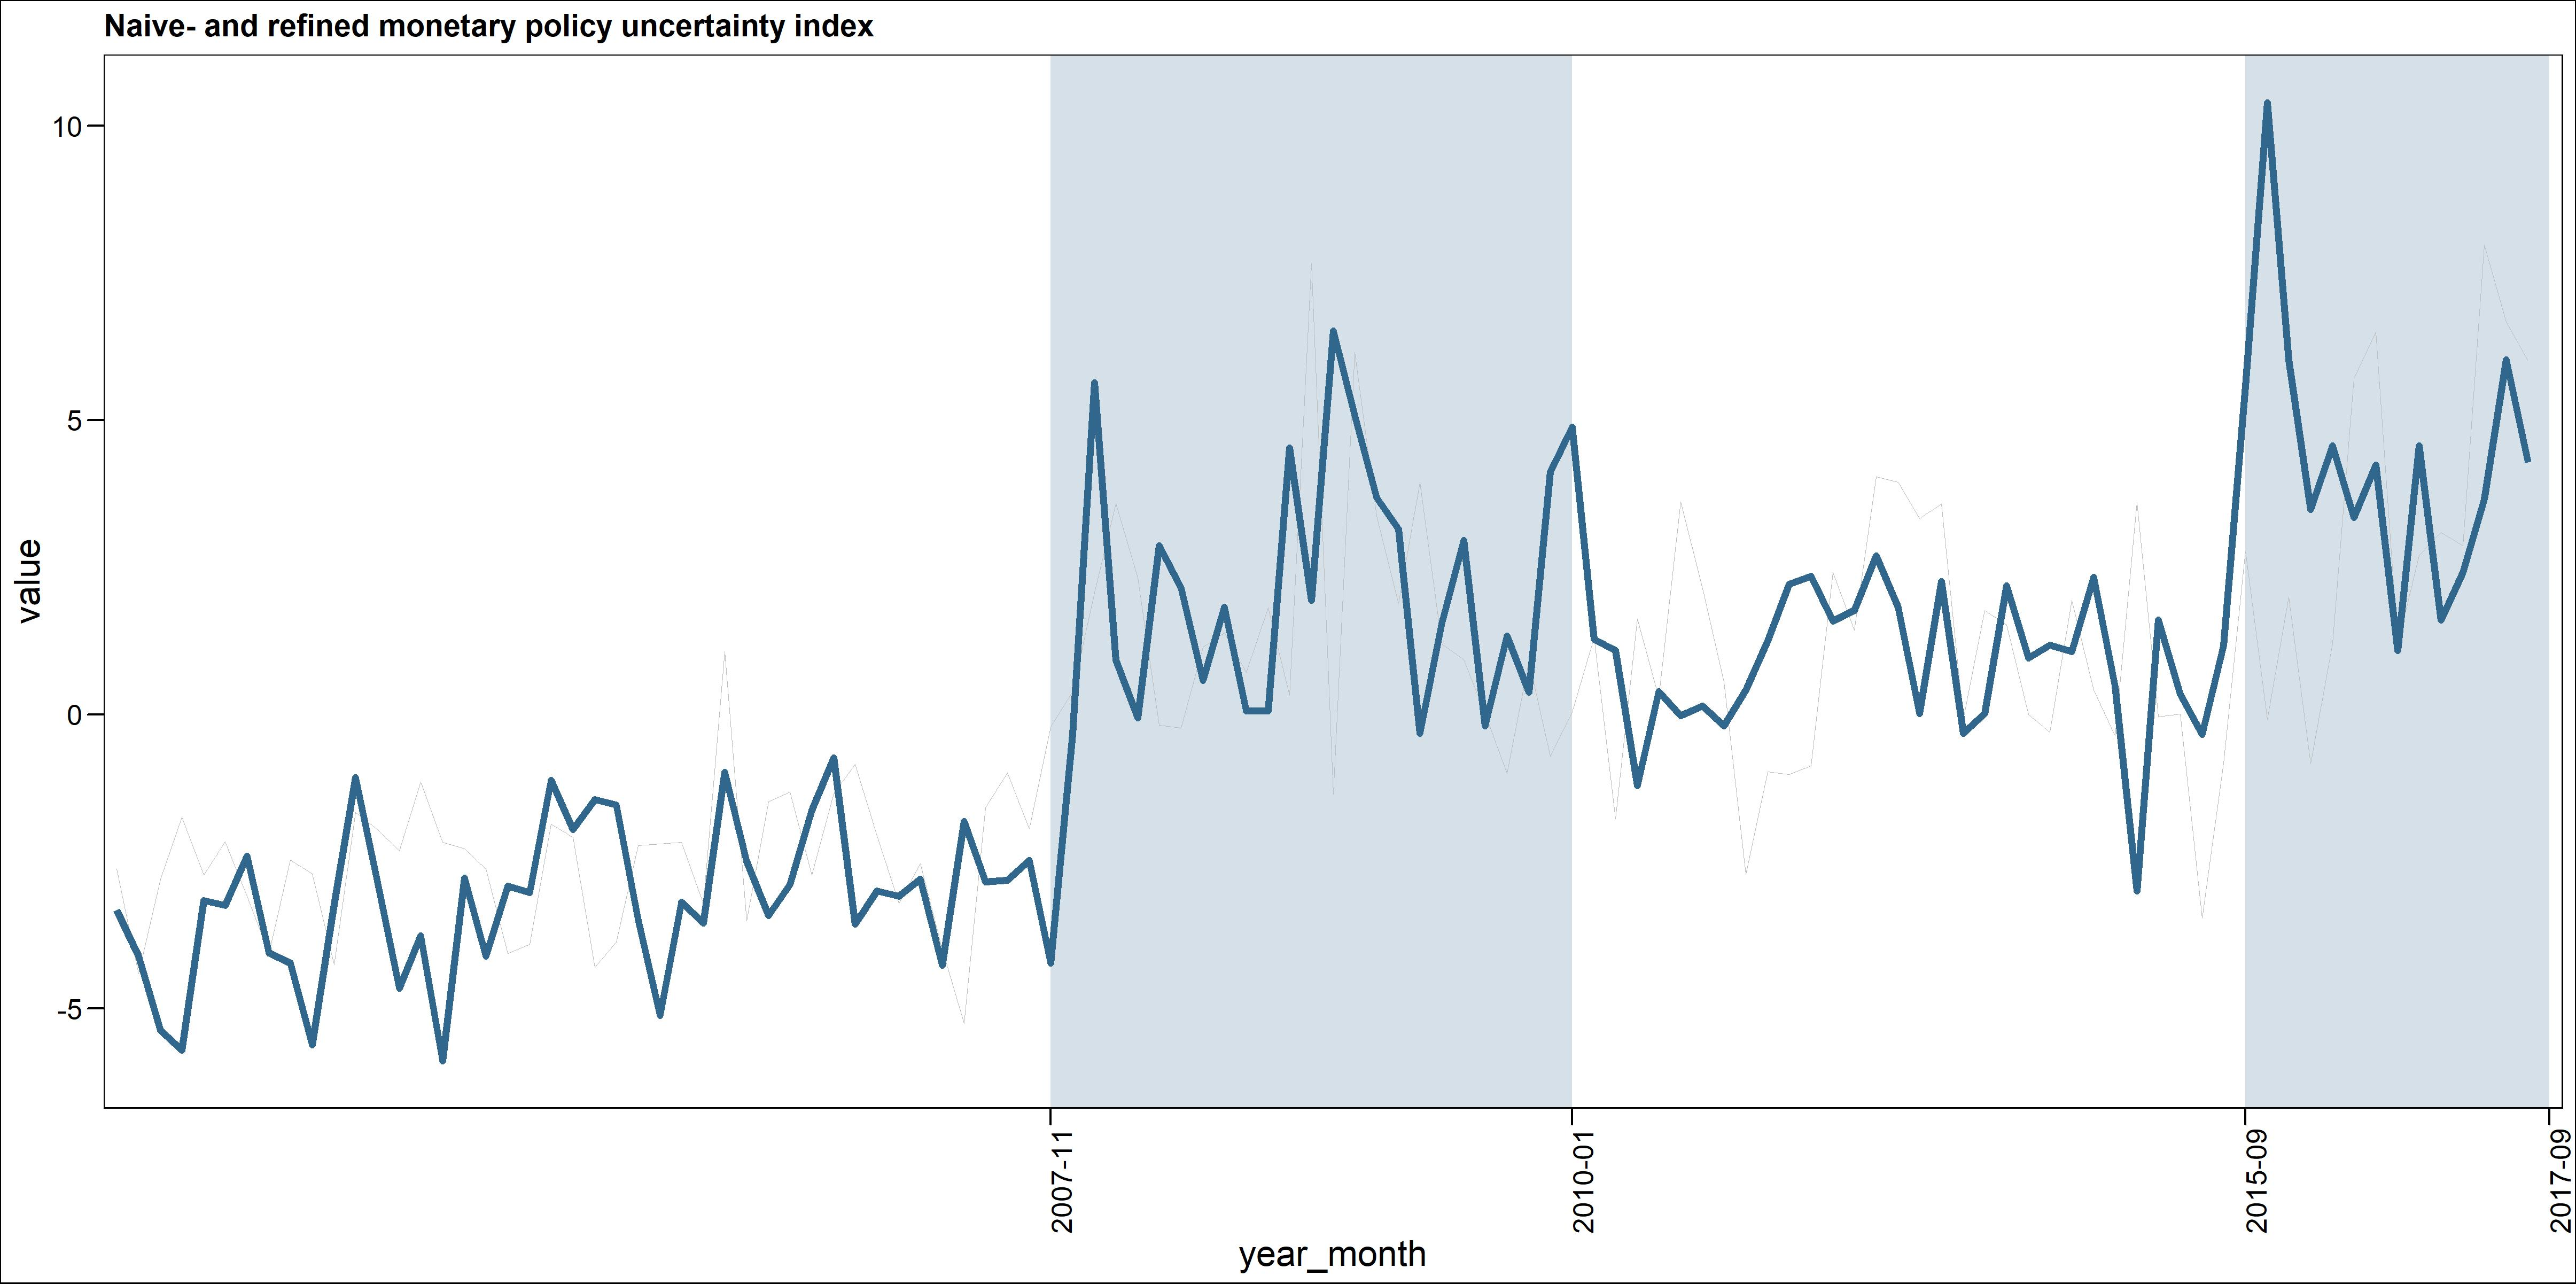
\includegraphics[width=\linewidth, keepaspectratio]{bin/monetary_comps}\\
	\caption{Composite Monetary Policy uncertainty refined index.\label{mon_comp_final}}
\end{figure}



\begin{figure}
	\centering
	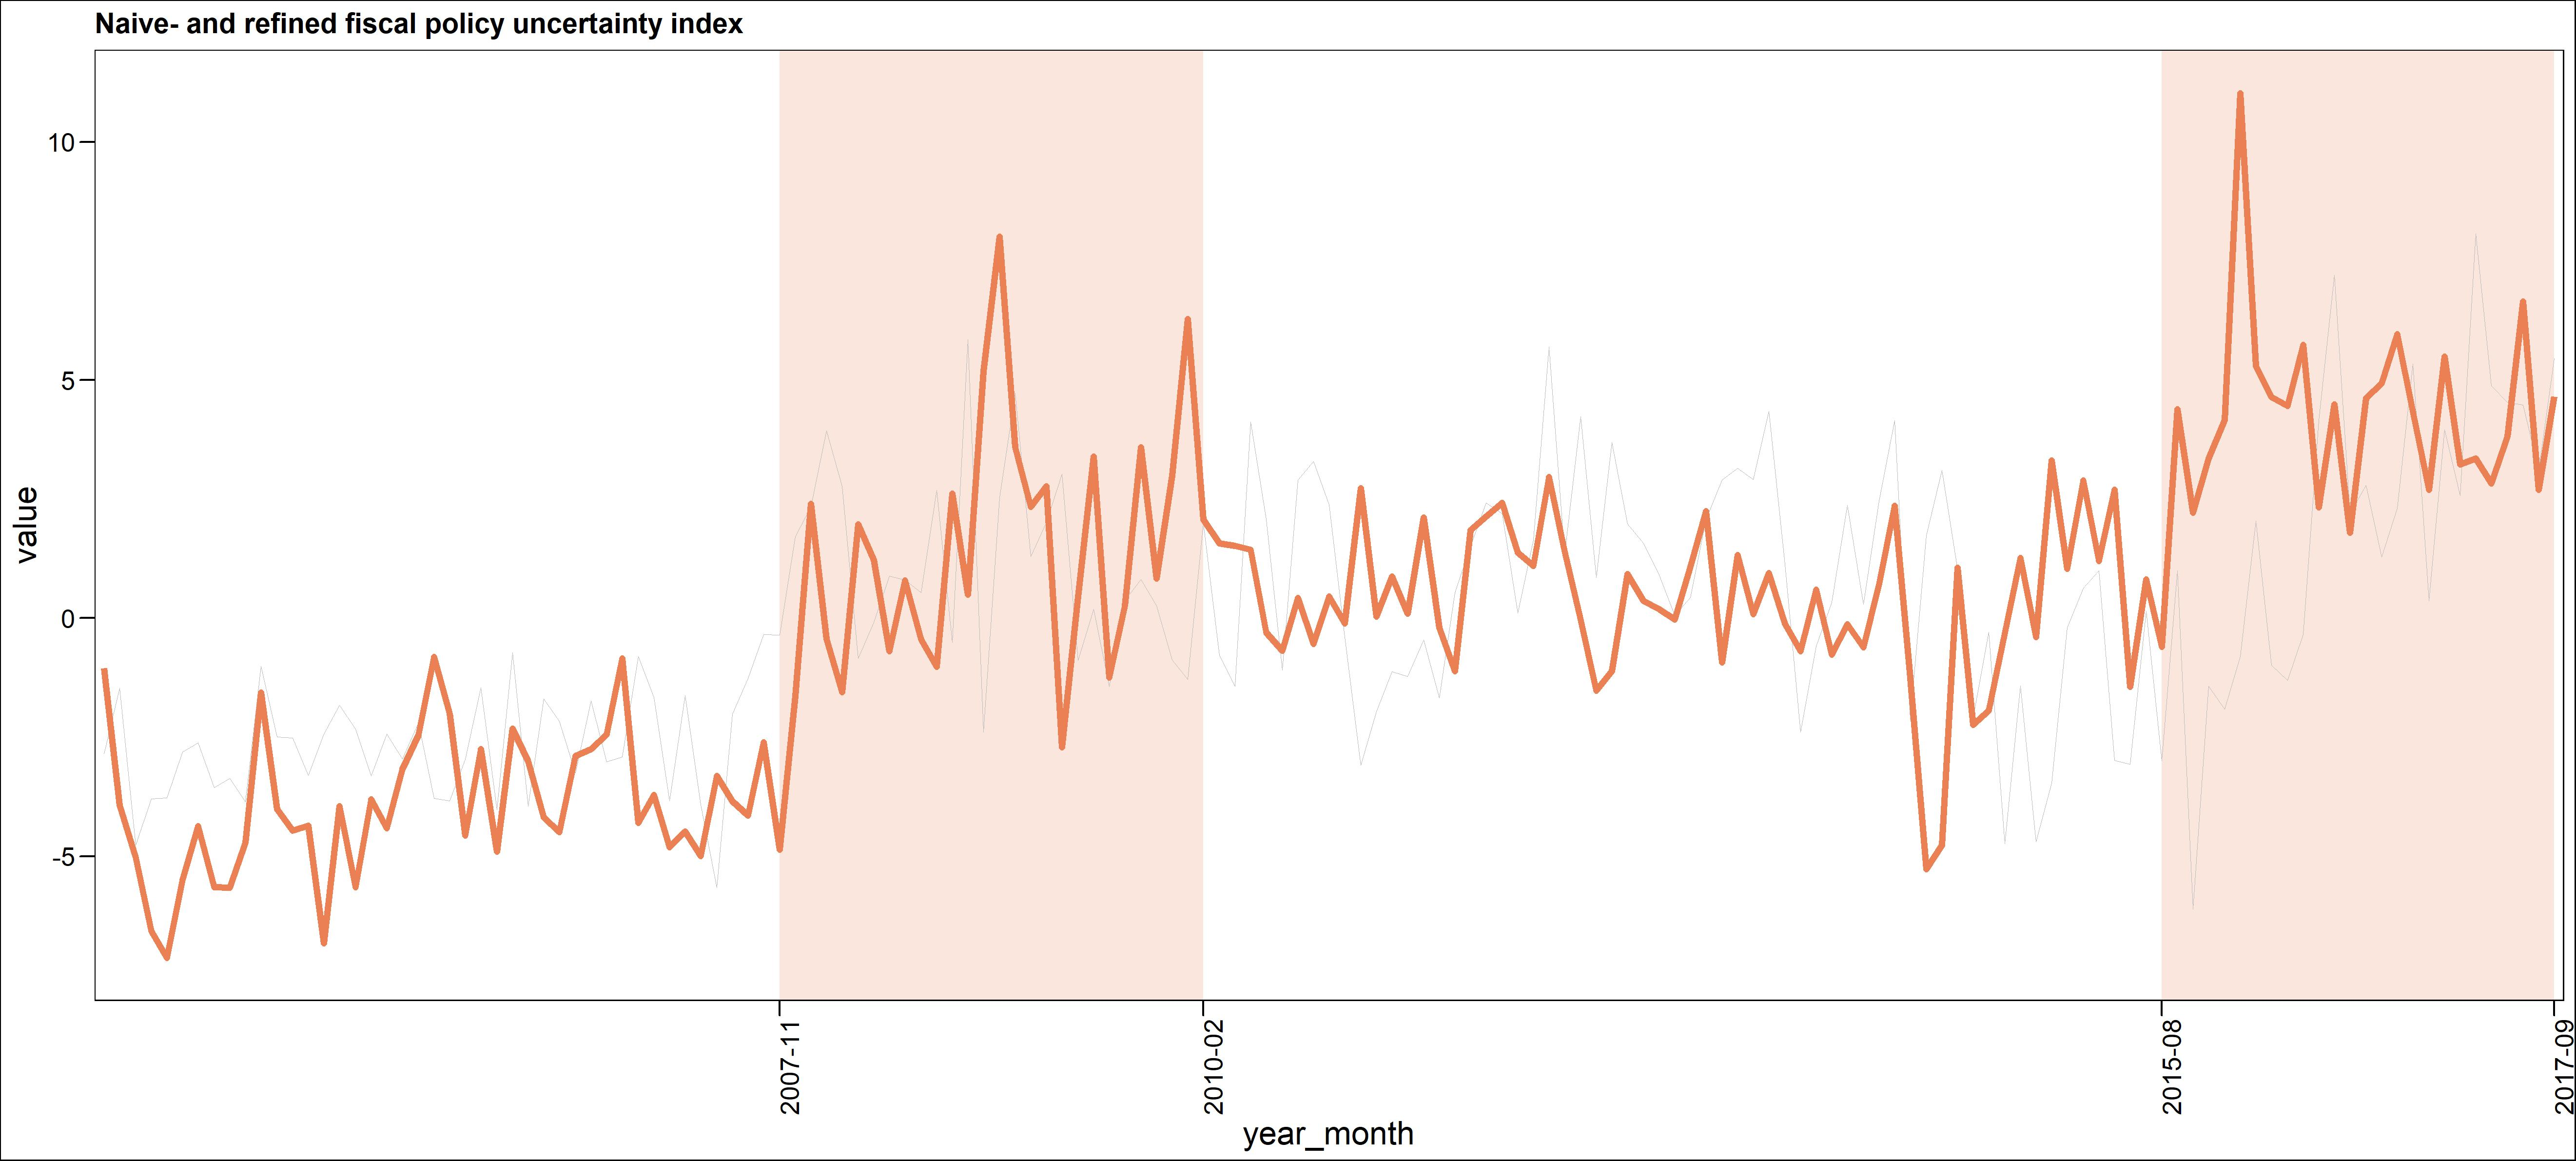
\includegraphics[width=\linewidth, keepaspectratio]{bin/fiscal_comps}\\
	\caption{Composite Fiscal Policy uncertainty refined index. \label{fis_comp_final}}
\end{figure}


\begin{figure}
	\centering
	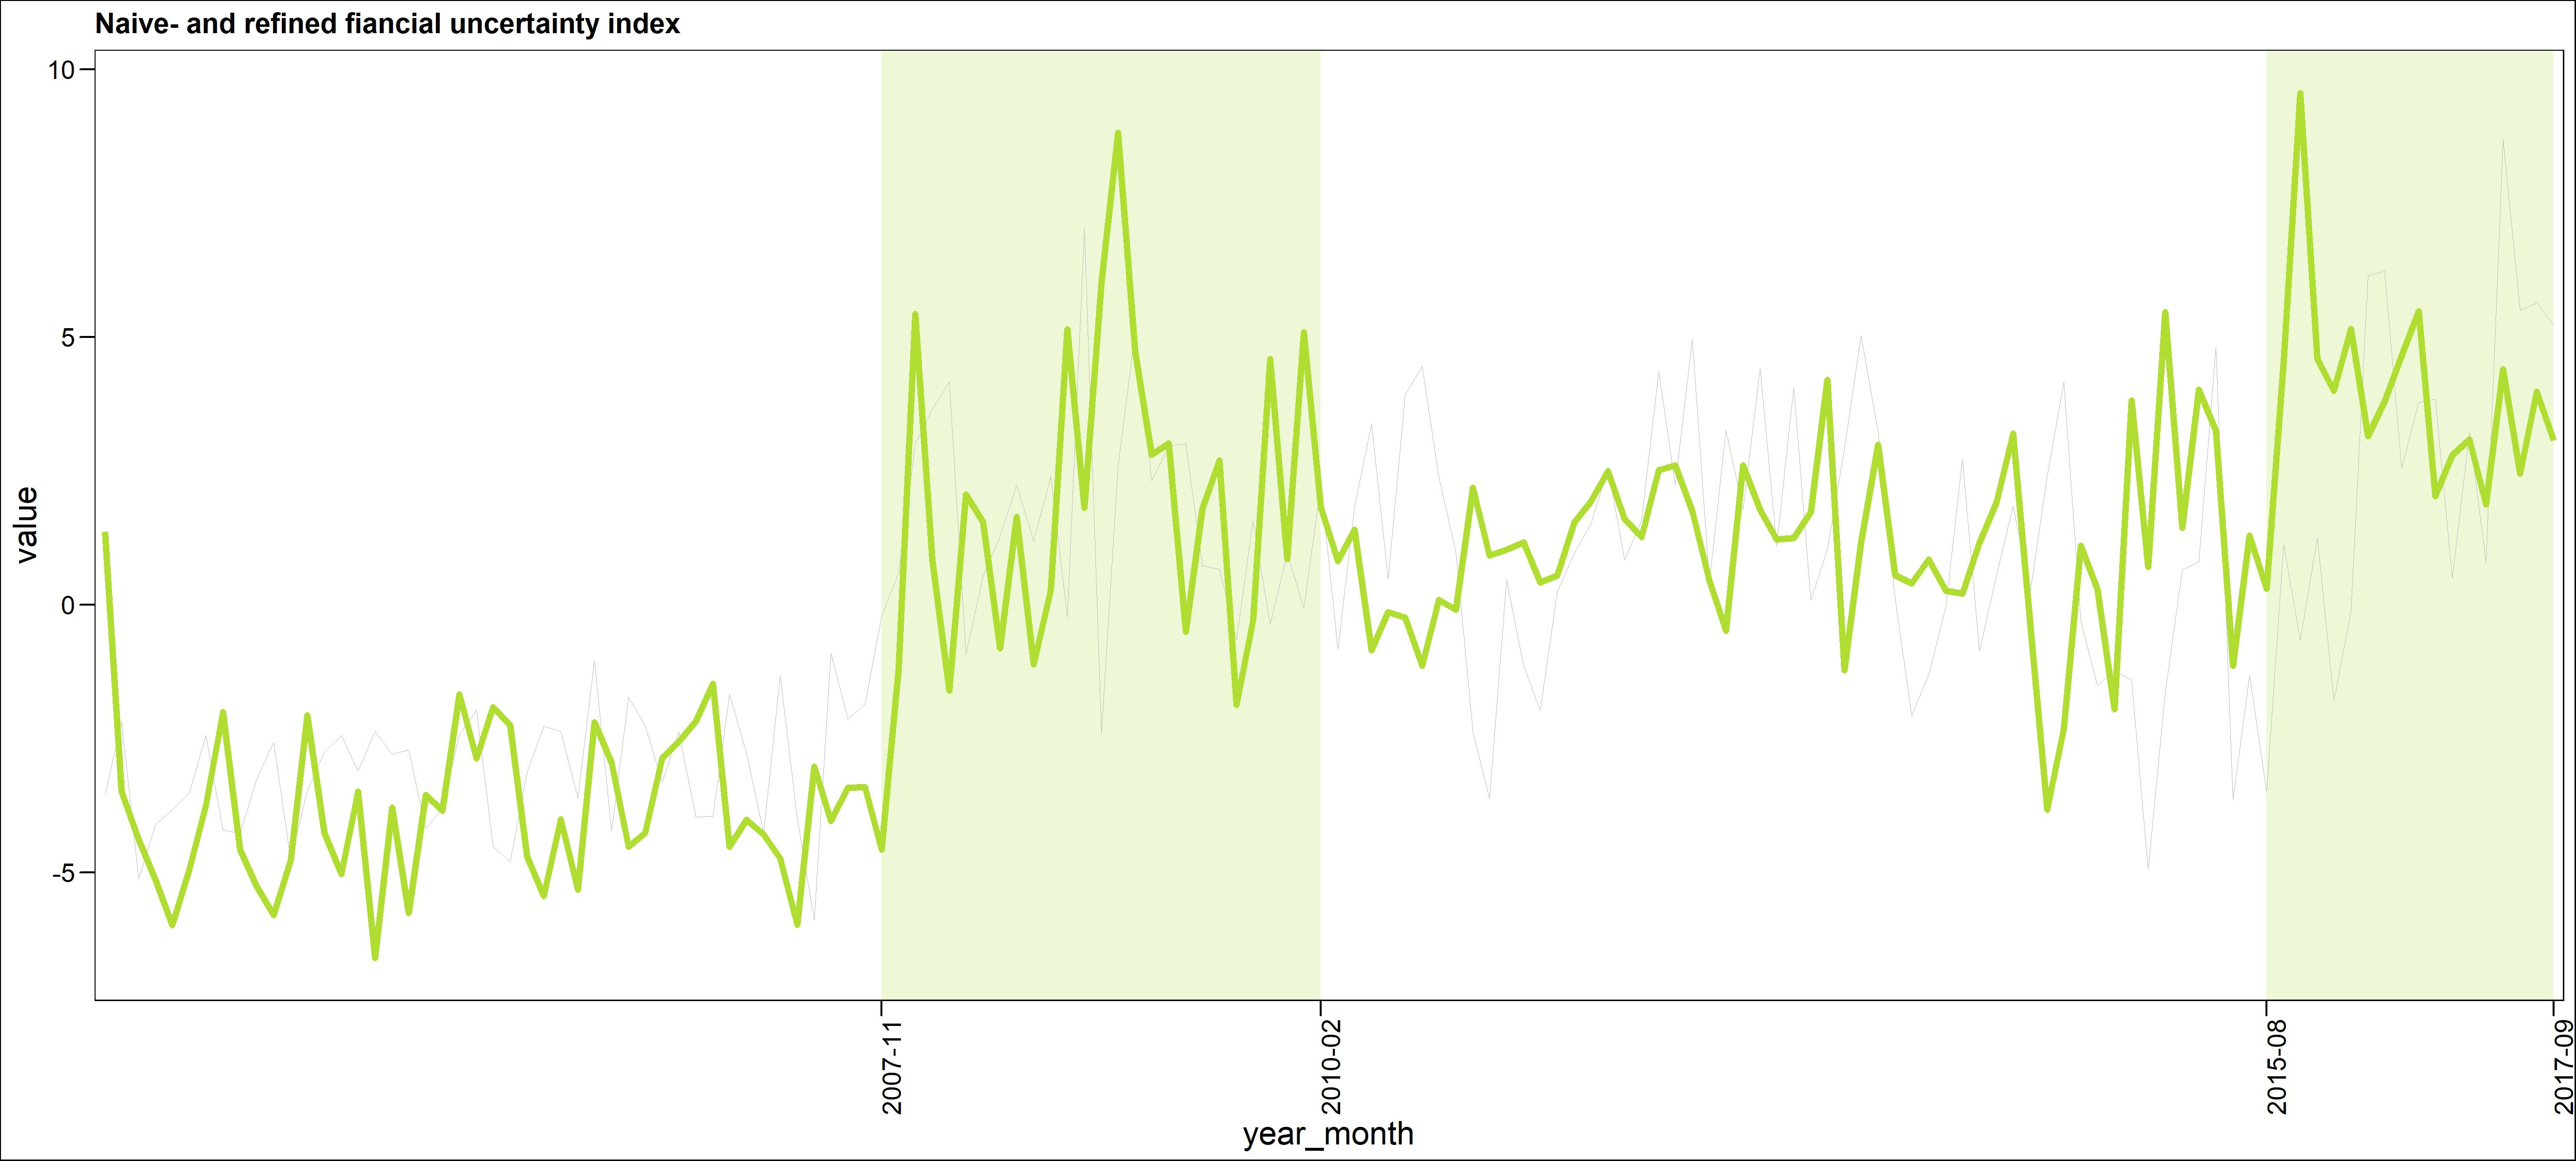
\includegraphics[width=\linewidth, keepaspectratio]{bin/financial_comps}\\
	\caption{Composite Financial market uncertainty refined index. \label{fin_comp_final}}
\end{figure}



\begin{figure}
	\centering
	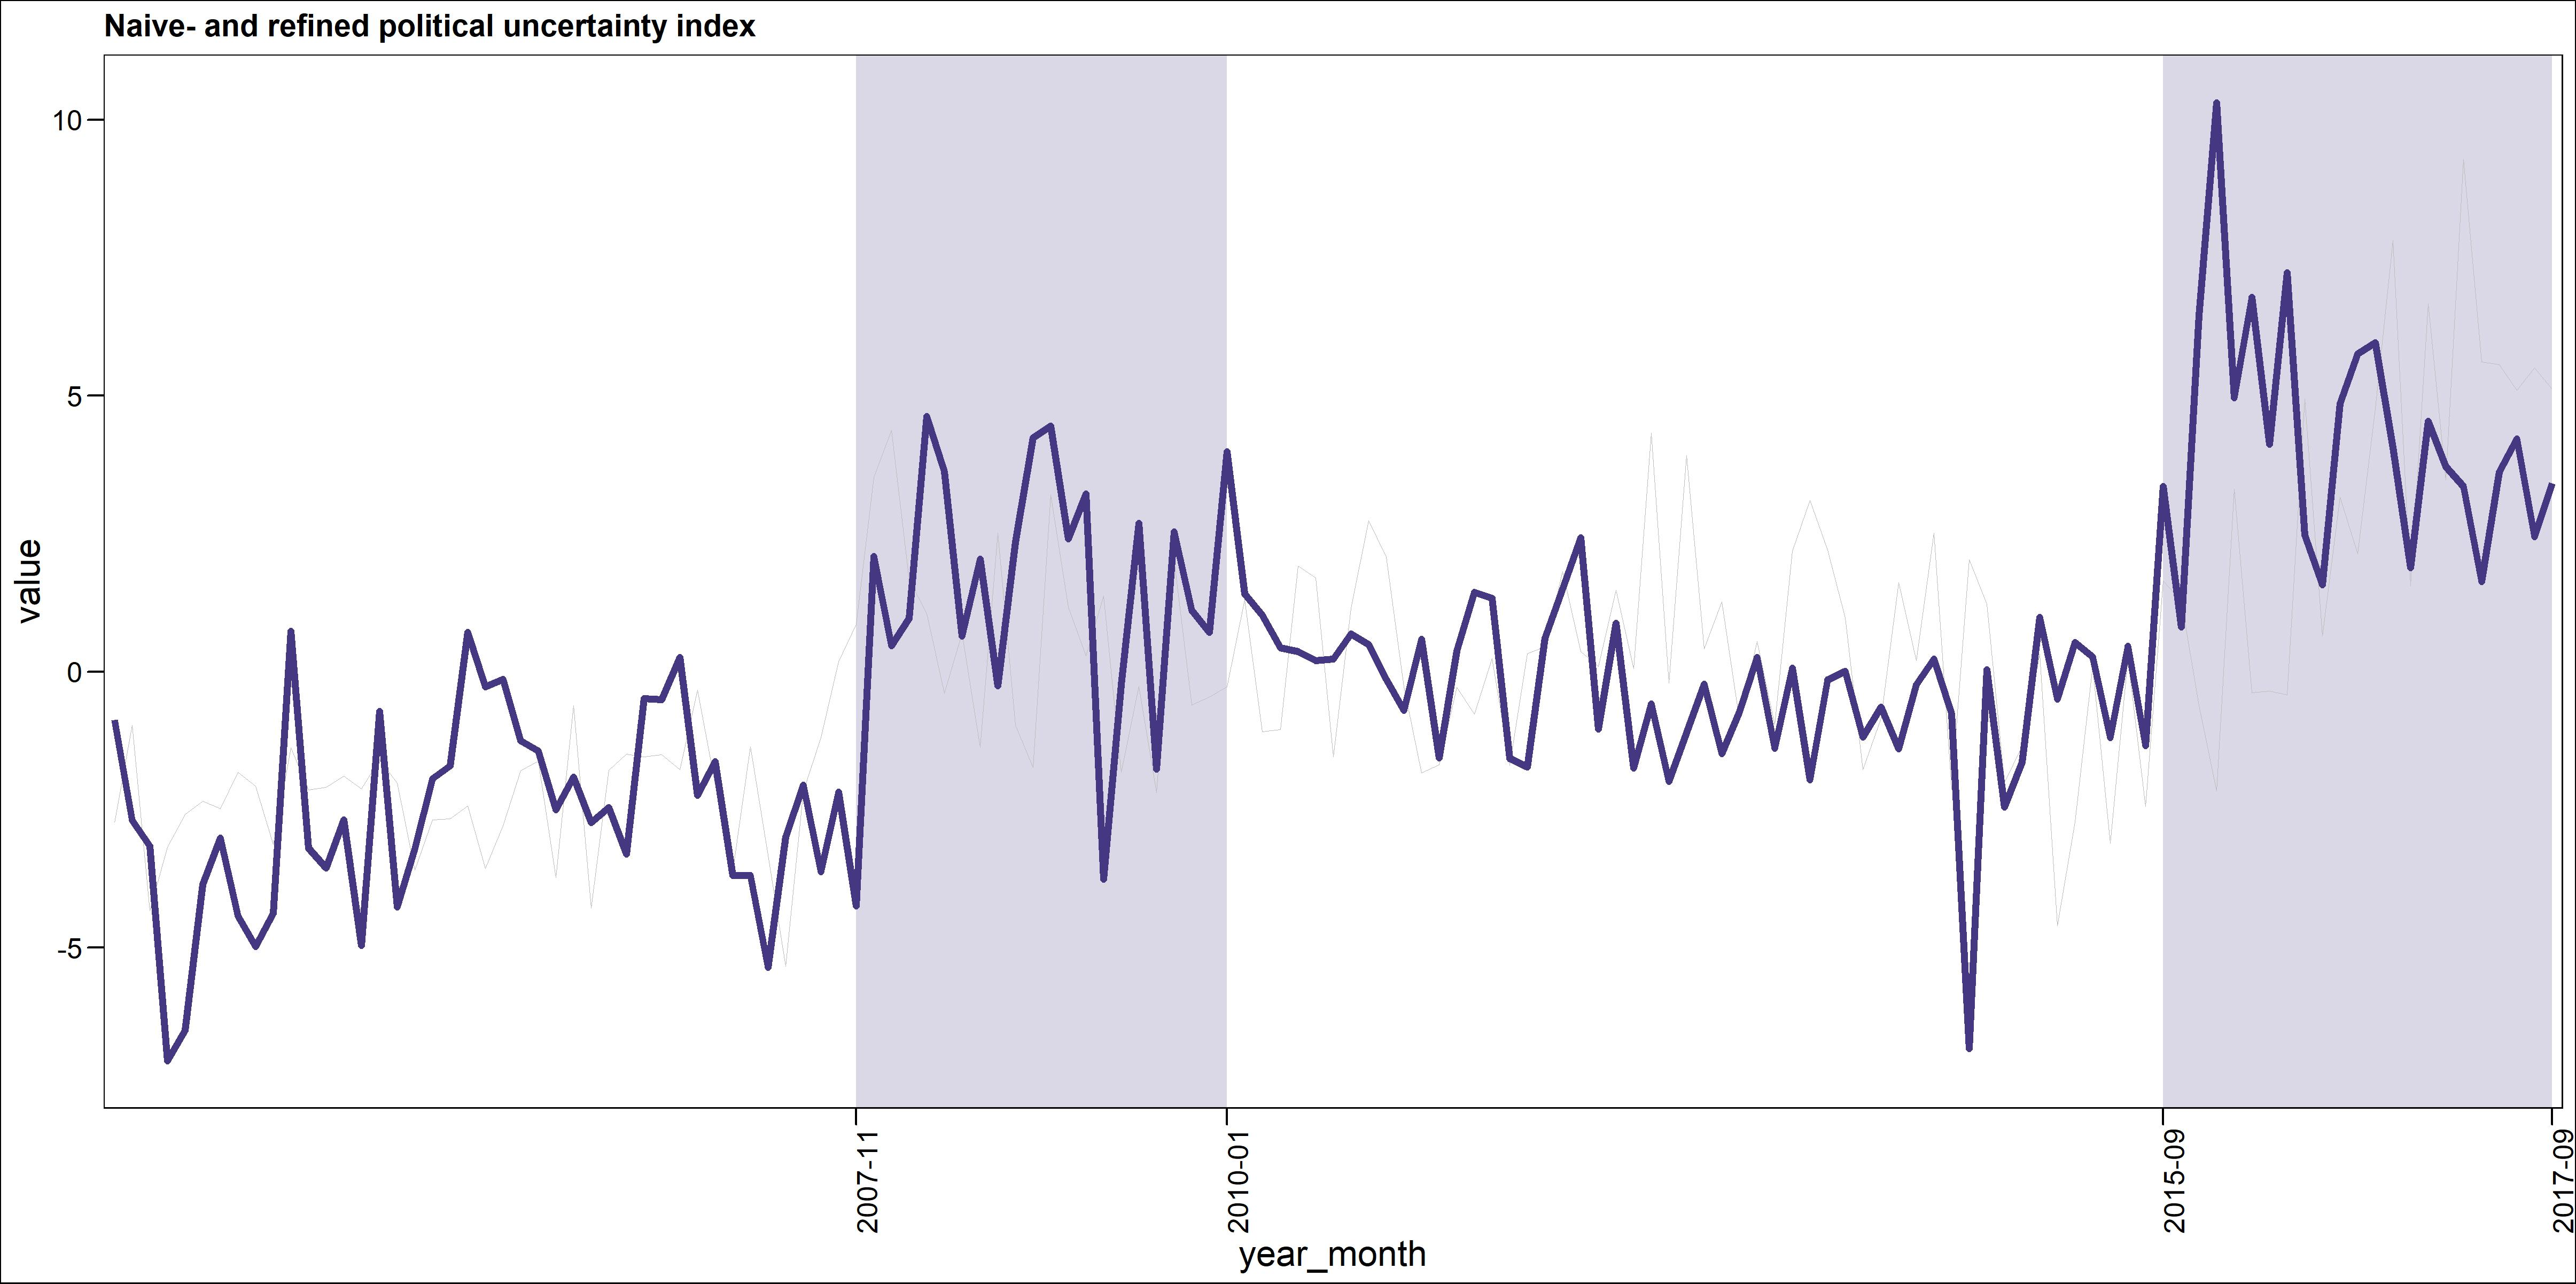
\includegraphics[width=\linewidth, keepaspectratio]{bin/pol_comps}\\
	\caption{Composite Political uncertainty refined index. \label{pol_comp_final}}
\end{figure}

\subsection{November 2007 to February
2010}\label{november-2007-to-february-2010}

Despite the lingering uncertainty regarding the GFC, one story dominated
the South African news in the last two months of 2007: the succession
race for the leadership of the ANC. Media reported that the deep divide
between a pro-Mbeki and pro-Zuma camp was \emph{paralysing} for the
party. The end of 2007 saw Jacob Zuma elected as new president of the
ANC. Shortly after his election, the National Prosecuting Authority
(NPA) brought new corruption charges against Zuma which caused the
pro-Zuma camp to call for the charges to be dropped, further dividing
the ANC.

Entering 2008, the divide in the ANC became ever increasing as Zuma's
trial took center stage in January. Uncertainty ruled about the policy
plan of the new leadership that some described as
\emph{populists, careerists and convicted criminals}. In the same month,
the effects of the GFC were seen in financial markets as it was reported
that collective investment inflows decreased by R10 billion in the last
quarter of 2017. Along with this, there was uncertainty on the fiscal
front as the auditor-general's office expressed concerns that the
funding model will result in unsustainable deficits.

At the start of the second quarter of 2008, South Africa faces two
crises. In what is described as a global food price crisis, cost of
living in South Africa reaches record levels hurting the poor. Coupled
with this, South Africa experiences a power crisis with Eskom asking the
energy regulator, NERSA, to allow the electricity price to double over
the following two years. Media reports that these crises threaten the
Reserve Bank's policies as they argue that domestic monetary policy is
ineffective in addressing fuel- and global food prices. There are
warnings that the inflation target might not be reached for as long as
two years. In the height of the cost of living crisis, media reports
about vehicle repossession rates increasing between 30 and 40\%.

The second quarter of 2008 also saw increased criticism of President
Mbeki as many became frustrated with his inaction regarding key issues
in the country. These issues include the crises discussed above, but
refers more specifically to the crisis in Zimbabwe and the future of the
Scorpions in South Africa. Mbeki infamously commented that ``there is no
crisis'' while referring to election crisis in Zimbabwe. His
relationship with Robert Mugabe also came into question during this
time. Moreover, critics of Mbeki condemned his handling of a report
recommending that the Scorpions not be incorporated into the national
police service. The pressure on Mbeki certainly started mounting during
this time and uncertainty about his future as head of state rose.

The last five months of 2008 saw many of the events that started out the
year, reach a climatic end. In terms of the price crises, August kicked
off with a mass strike by Cosatu and 21 of its affiliates in protest of
high prices. More than 100 000 workers joined all across the country.
Merely a week later, Eskom applies for another price hike after NERSA
turned down an application for a 53\% price increase. In October, the
energy provider wins a major battle with regards to a pricing rule
changes that enable Eskom to treat primary energy as a pass-through
cost. Amid higher inflation and weaker Rand, uncertainty regarding the
applicability of inflation targeting also arises. This necessitates the
Governer of the Reserve Bank, Tito Mboweni to defend the policy. By the
end of 2008, the Bank faces a dilemma as the current account deficit
widens rendering a interest rate cut unpopular.

In the last five months of 2008, the divide in the ANC increased as the
pro-Zuma camp called for the trial against him to be stopped. In
September, Mbeki suffers a major defeat as the NPA dismissed the case
against Zuma with Judge Nicholson admitting to the NPA being influenced
by political masters. On the 25th of September Kgalema Motlanthe is
sworn in as president following the resignation of Mbeki. Despite Judge
Nicholson's finding being the catalyst for Mbeki's recall, the ANC did
not take disciplinary action against the ousted president.

Uncertainty about the two camps in the ANC party also reached a climax
by the end of 2008. Already in October, media reported of a
\emph{separatist storm brewing}. Several ministers resigned following
the recall of Mbeki with former defence minister, Mosuioa Lekota
becoming the unofficial leader of the ANC dissidents. By the end of
October a national convention to discuss the possible formation of a new
political party has been organised. However, the planned convention did
not provide more certainty in the economy as Mbeki wrote a letter in
which he pledged his continued support for the ANC and disapproved of
the formation of the new party. Notwithstanding, the
\emph{Congress of the people (COPE)} party is formed on the 16th of
December.

In 2009, in the wake of the split in the party, the ANC was left to
rebuild its name and show that it is united as the election drew closer.
A setback came early in January when the Supreme Court of Appeal (SCA)
overturned and heavily criticised Judge Nicholson's finding on Zuma's
corruption trial. Uncertainty about these events ruled for the entire
first quarter of 2016 with both opposition and supporters of Zuma
enjoying extensive coverage in the media. In the closing of this case in
April, the NPA was left to explain why they decided to drop the charges
against Zuma after almost a decade of on-and-off investigation. The NPA
cited political interference and manipulation as reasons for the
decision.

The dismissal of Zuma's case in April came just before the general
election in which the ANC won. However, the defeat was preceded by four
months of political rivalry with the newly formed COPE party. COPE faced
off directly with the ANC holding rallies in the Eastern Cape,
KwaZulu-Natal and North West. The outcome of the NPA's decision
regarding Zuma's trial, however, did not count in COPE's favour. In May,
Zuma was elected as President by parliament.

Amid the uncertainty on the political landscape, the first four months
of 2009 was also characterised by increased concerns over the global
economy. Particularly in South Africa, rising unemployment was set to
keep consumer spending low and private investment was not picking up. In
February, Treasury warned that the state of the economy could still
worsen and that a recession is not unlikely. The Reserve Bank's
inflation targeting policy again came under fire as arguments about its
appropriatness was critised. By March it was almost certain that South
Africa will be in a recession before the end of the year as the global
economy struggled after the GFC.

The last six months of 2009 was considerably less uncertain with only
three months showing spikes in figures \ref{mon_comp_final} to
\ref{pol_comp_final}. The news in July was dominated by a realising of
the full effect of the economic downturn. In his first budget vote
speech, Finance Minister Pravin Gordhan told parliament that South
Africa's growth path for the next several years looks grim. Stats South
Africa reported that more than 250 000 of jobs were lost during the
second quarter of 2009 and that more than 302 000 discouraged job
seekers stopped looking for jobs. This coincided with countrywide
protests over poor wage increases.

In October, uncertainty ruled regarding the medium-term budget. South
Africa needed a prudent budget to navigate the difficult economic
environment. There was not uncertainty about Gordhan's ability to draft
such a budget, but the media reported the scepticism of opposition
parties regarding Gordhan's \emph{political muscle} to convince the
cabinet. This was especially pertinent since this would be the first
time that Parliament would have the power to change the budget.

The end of 2009 was characterised by Eskom requesting historic
electricity price increases. A document containing Eskom's request for a
45\% increase was leaked after Parliament tried to keep the application
hidden. Media reported on the uncertain effect that such a large
increase would have on South Africa's growth path. By the end of the
year, reports surfaced claiming the hikes could cost the economy R150
billion.

Media speculated that 2010 will be a turbulent year as a number of
contentious bills were set to be debated. However, figures
\ref{mon_comp_final} to \ref{pol_comp_final} show that all four indices
show less uncertainty after the second month of 2010. This is likely a
result of the 2010 Fifa Soccer World Cup dominating news stories for the
biggest part of 2010. One other thing that did enjoy extensive coverage
is Eskom's continued plea for a price increase. In January 2010 NERSA
held public hearings on Eskoms' application for a 35\% price increase
over the following three years. At the end of February, NERSA granted
hikes of only 25\% for the following three years, forcing Eskom to
borrow on the open market.

\subsection{August 2015 to July 2017}\label{august-2015-to-july-2017}

The last five months of 2015 was characterised by extreme political
volatility in South Africa. The period started out with uncertainty
about the Monetary Policy Committee's (MPC) decision regarding the
instrument rate. Amid unfavourable economic conditions such as high
unemployment, \emph{Fees must Fall}- and wage inequality strikes and
concerns about rising debt levels, it was not sure whether the MPC will
increase the repo rate or leave it unchanged. These conditions on their
own were also a source of uncertainty as newspapers speculated about the
impact of the economic downturn. In this period, the news was also
dominated by uncertainty regarding the future of electricity supply in
South Africa. In particular, the discussions in parliament regarding the
proposed nuclear programme enjoyed extensive coverage in the news.

One big event caused all four indices to show the biggest spike in
uncertainty at the end of 2015: the replacement of Minister of Finance
Nhlanhla Nene, with a relatively unknown figure, David van Rooyen. This
shock came amid already rising concerns for a credit ratings downgrade.
The nuclear procurement programme was approved by cabinet shortly after
the replacement of Nene as minister. Giving in to mounting pressure from
various agents, President Jacob Zuma replaced David van Rooyen with
Pravin Gordhan after only four days as finance minister. This went a
long way in lowering uncertainty in the subsequent month, but the level
of uncertainty remained high for 2016 and 2017 compared to before
September 2015.

In 2016, \emph{Fees must Fall} protests continue with the start of the
academic year with increased pressure on government to intervene.
Regardless, President Zuma's state of the nation address in February
2016 failed to provide certainty about the ruling party's proposed plans
to address the dire state of the economy and ongoing protests. Moreover,
during the first two months of 2016, there was considerable uncertainty
about the future of South Africa's sovereign credit rating as rating
agencies kept a close eye on minister Pravin Gordhan delivering the
budget speech at the end of February. The finance minister remained in
the news the following month with rumours of his arrest resulting from
an investigation by the Hawks into a ``rogue unit'' when he was
commissioner at the South African Revenue Services.

The second quarter of 2016 saw the Constitutional Court condemn
President Zuma's handling of the Public Protector Thuli Madonsela's
report on improvements to the president's private property, Nkandla. The
court's finding increased calls for Zuma's resignation. The news
referred to this time as a \emph{deep political crisis} for the ruling
party. Uncertainty ruled about the voting process in a motion of no
confidence against the president after the party decided to support Zuma
in a meeting of the party's top six officials. These events had a
significant impact on the financial markets with the Rand losing ground
against the Dollar and fear of a credit rating downgrade increasing. By
the end of the quarter uncertainty decreased (also seen in figures
\ref{mon_comp_final} to \ref{pol_comp_final}) with reports about the
possibility of a downgrade being less frequent.

In the third quarter of 2016 the political landscape in South Africa
seems to calm down. This notwithstanding the municipal elections in
August which does not show an increase in the indices to the extent that
is seen in the previous quarter. This is likely due to the extensive
coverage of the results of the Brexit referendum in the news. In
September, President Zuma pays back the money owed according to the
Public Protector's report for the upgrades to Nkandla. Apart from the
normal coverage of the MPC's decision regarding the repo rate, this
quarter ends on a considerably less uncertain note.

The end of 2016 was characterised by renewed uncertainty about a looming
credit rating downgrade. Early in the final quarter of 2016 multiple
reports issued by among other, previous Minister of Finance Trevor
Manuel as well as Pravin Gordhan warned against deviating from the
fiscal targets set in the February budget. This was amid ongoing
investigations into minister Gordhan who was preparing the medium-term
budget speech that was sure to play a key part in the ratings agencies'
decision. Despite markets expecting a one notch downgrade, all three
rating agencies placed South Africa on a negative outlook for one year.
Charges against minister Gordhan were dropped at the end of October.

A second report released by Public Protector Thuli Madonsela at the end
of 2016 proved to set the stage for a number of events in 2017. The
report concerned President Zuma's involvement in and the extent of state
capture in South Africa. However, the ANC again stood by Zuma calling
the report inconclusive.

At the start of 2017, the extent of the Gupta family's involvement in
state capture became more clear as a public battle for treasury played
out. The Gupta-owned company, Oakbay Investments released an affidavit
accusing minister Gordhan of using the judiciary for own political gain.
Media started speculating that another cabinet reshuffle is on the cards
that will see the removal of Pravin Gordhan as Finance minister. In
February, the annual State of the Nation Address was the most chaotic in
recent history. After the forced removal of the EFF party, the DA and
COPE also left the House. Zuma delivered an underwhelming address that
failed to speak to the country's biggest economic problems to the
remaining members of parliament.

Uncertainty regarding the VAT rate leading up to Gordhan's budget speech
was reported on during February. Agents argued that this was the only
way to finance a growing budget deficit. The budget speech laid
speculation to rest when Gordhan announced that the rate will remain
unchanged. Following the budget speech, uncertainty regarding the growth
forecasts was widely reported on. In March, rating agencies reiterated
concerns about the optimistic forecasts and political instability in the
country. This sparked reporting on a possible credit rating downgrade
which affected the financial markets. By the end of March, media
reported that both Gordhan and his deputy, Mcebisi Jonas, are set to be
replaced in another cabinet reshuffle.

The start of the second quarter of 2017 was introduced with a cabinet
reshuffle just after midnight on 30 March. Following months of
speculation, a new minister- and deputy minister of finance was
announced by President Zuma. A credit rating downgrade by Fitch followed
in early April causing an increase in uncertainty for all four indices
in figures \ref{mon_comp_final} to \ref{pol_comp_final}. Uncertainty
about whether the remaining two rating agencies will follow suit and
what the full effect of this would be was covered extensively in the
media. These reports dominated the news in April along with uncertainty
about the new Finance Minister Malusi Gigaba.

In the last three months of the identified period, Zuma's opposition
became more as well as more vocal. Lobby groups and business leaders
challenged the most recent cabinet changes as all eyes were on the new
Finance Minister. Speculation of yet another motion of no confidence
against Zuma also enjoyed coverage in the news. In this time, there is
also uncertainty about the policy direction that the ANC is set to take
as reports about wide-spread state capture kept surfacing. This
political instability coupled with low economic growth is given as the
reason for Moody's downgrading South Africa's debt to junk status
mid-June.

A face-off between new Public Protector Busisiwe Mkhwebane and the
Reserve Bank was another major cause of uncertainty during this period.
The Public Protector called for a revision of the mandate of the Reserve
Bank to focus on the socio-economic wellbeing of South Africans. Markets
reacted promptly to the possibility of interference with the Bank with
the Rand losing major ground against the Dollar. This event enjoyed
extensive coverage in the media with responses from Reserve Bank
Governor, Lesetja Kganyago, as well as various influential academics and
economists.

In the background, uncertainty about another political event grew: the
race for the presidency of the ANC party. Media coverage about the ANC
elective conference to be held December 2017 began early in 2017 already
with wide-spread uncertainty about the policy agenda of the ANC as well
as the candidates.

\section{\texorpdfstring{Conclusion
\label{sec_conclude}}{Conclusion }}\label{conclusion}

\newpage

\section*{References}\label{references}
\addcontentsline{toc}{section}{References}

\hypertarget{refs}{}
\hypertarget{ref-2016}{}
``2016 in Review.'' 2016. \emph{South African History Online}.
\url{https://www.sahistory.org.za/article/2016-review}.

\hypertarget{ref-Azqueta-Gavaldon2017}{}
Azqueta-Gavaldón, Andrés. 2017. ``Developing News-Based Economic Policy
Uncertainty Index with Unsupervised Machine Learning.'' \emph{Economics
Letters} 158 (September): 47--50.
doi:\href{https://doi.org/10.1016/j.econlet.2017.06.032}{10.1016/j.econlet.2017.06.032}.

\hypertarget{ref-Bachmann2013}{}
Bachmann, Rüdiger, Steffen Elstner, and Eric R Sims. 2013. ``Uncertainty
and Economic Activity: Evidence from Business Survey Data.''
\emph{American Economic Journal: Macroeconomics} 5 (2): 217--49.
doi:\href{https://doi.org/10.1257/mac.5.2.217}{10.1257/mac.5.2.217}.

\hypertarget{ref-Baker2016}{}
Baker, Scott R., Nicholas Bloom, and Steven J. Davis. 2016. ``Measuring
Economic Policy Uncertainty.'' \emph{The Quarterly Journal of Economics}
131 (4): 1593--1636.
doi:\href{https://doi.org/10.1093/qje/qjw024}{10.1093/qje/qjw024}.

\hypertarget{ref-Bloom2014}{}
Bloom, Nicholas. 2014. ``Fluctuations in Uncertainty.'' \emph{Journal of
Economic Perspectives} 28 (2): 153--76.
doi:\href{https://doi.org/10.1257/jep.28.2.153}{10.1257/jep.28.2.153}.

\hypertarget{ref-Caggiano2014}{}
Caggiano, Giovanni, Efrem Castelnuovo, and Nicolas Groshenny. 2014.
``Uncertainty Shocks and Unemployment Dynamics in U.S. Recessions.''
\emph{Journal of Monetary Economics} 67 (October): 78--92.
doi:\href{https://doi.org/10.1016/j.jmoneco.2014.07.006}{10.1016/j.jmoneco.2014.07.006}.

\hypertarget{ref-Caldara2016}{}
Caldara, Dario, Cristina Fuentes-Albero, Simon Gilchrist, and Egon
Zakrajšek. 2016. ``The Macroeconomic Impact of Financial and Uncertainty
Shocks.'' \emph{European Economic Review} 88 (September): 185--207.
doi:\href{https://doi.org/10.1016/j.euroecorev.2016.02.020}{10.1016/j.euroecorev.2016.02.020}.

\hypertarget{ref-Hardouvelis2018}{}
Hardouvelis, Gikas A., Georgios Karalas, Dimitrios Karanastasis, and
Panagiotis Samartzis. 2018. ``Economic Policy Uncertainty, Political
Uncertainty and the Greek Economic Crisis.'' \emph{SSRN Electronic
Journal}.
doi:\href{https://doi.org/10.2139/ssrn.3155172}{10.2139/ssrn.3155172}.

\hypertarget{ref-Jurado2015}{}
Jurado, Kyle, Sydney C. Ludvigson, and Serena Ng. 2015. ``Measuring
Uncertainty.'' \emph{American Economic Review} 105 (3): 1177--1216.
doi:\href{https://doi.org/10.1257/aer.20131193}{10.1257/aer.20131193}.

\hypertarget{ref-Kelly2016}{}
Kelly, Bryan, Ľuboš Pástor, and Pietro Veronesi. 2016. ``The Price of
Political Uncertainty: Theory and Evidence from the Option Market: The
Price of Political Uncertainty.'' \emph{The Journal of Finance} 71 (5):
2417--80.
doi:\href{https://doi.org/10.1111/jofi.12406}{10.1111/jofi.12406}.

\hypertarget{ref-Loughran2016}{}
Loughran, Tim, and Bill Mcdonald. 2016. ``Textual Analysis in Accounting
and Finance: A Survey: TEXTUAL ANALYSIS IN ACCOUNTING AND FINANCE.''
\emph{Journal of Accounting Research} 54 (4): 1187--1230.
doi:\href{https://doi.org/10.1111/1475-679X.12123}{10.1111/1475-679X.12123}.

\hypertarget{ref-Mekuto2017}{}
Mekuto, Dinilohlanga. 2017. ``Highlights of Stories in 2017.''
\url{http://www.sabcnews.com/sabcnews/2017s-biggest-stories/}.

\hypertarget{ref-Odendaal2018}{}
Odendaal, Nicolaas Johannes, and Monique Reid. 2018. ``Media Based
Sentiment Indices as an Alternative Measure of Consumer Confidence.''
\emph{Stellenbosch Economic Working Papers} WP17/2018.

\hypertarget{ref-Ooms2017}{}
Ooms, Jeroen. 2017. ``Pdftools: Text Extraction, Rendering and
Converting of Pdf Documents.'' \emph{Computer Software Manual{]}.
Retrieved from Https://CRAN. R-Project. Org/Package= Pdftools}.

\hypertarget{ref-Pastor2013}{}
Pástor, Ľuboš, and Pietro Veronesi. 2013. ``Political Uncertainty and
Risk Premia.'' \emph{Journal of Financial Economics} 110 (3): 520--45.
doi:\href{https://doi.org/10.1016/j.jfineco.2013.08.007}{10.1016/j.jfineco.2013.08.007}.

\hypertarget{ref-Redl2015}{}
Redl, Chris. 2015. ``Macroeconomic Uncertainty in South Africa,'' 34.

\hypertarget{ref-2018}{}
``South Africa Profile - Timeline.'' 2018. \emph{BBC News}.
\url{https://www.bbc.com/news/world-africa-14094918}.

\hypertarget{ref-Tobback2018}{}
Tobback, Ellen, Hans Naudts, Walter Daelemans, Enric Junqué de Fortuny,
and David Martens. 2018. ``Belgian Economic Policy Uncertainty Index:
Improvement Through Text Mining.'' \emph{International Journal of
Forecasting} 34 (2): 355--65.
doi:\href{https://doi.org/10.1016/j.ijforecast.2016.08.006}{10.1016/j.ijforecast.2016.08.006}.

\section*{\texorpdfstring{Appendix
		\label{sec_appendix}}{Results }}\label{appendix}
\begin{figure}
	\centering
	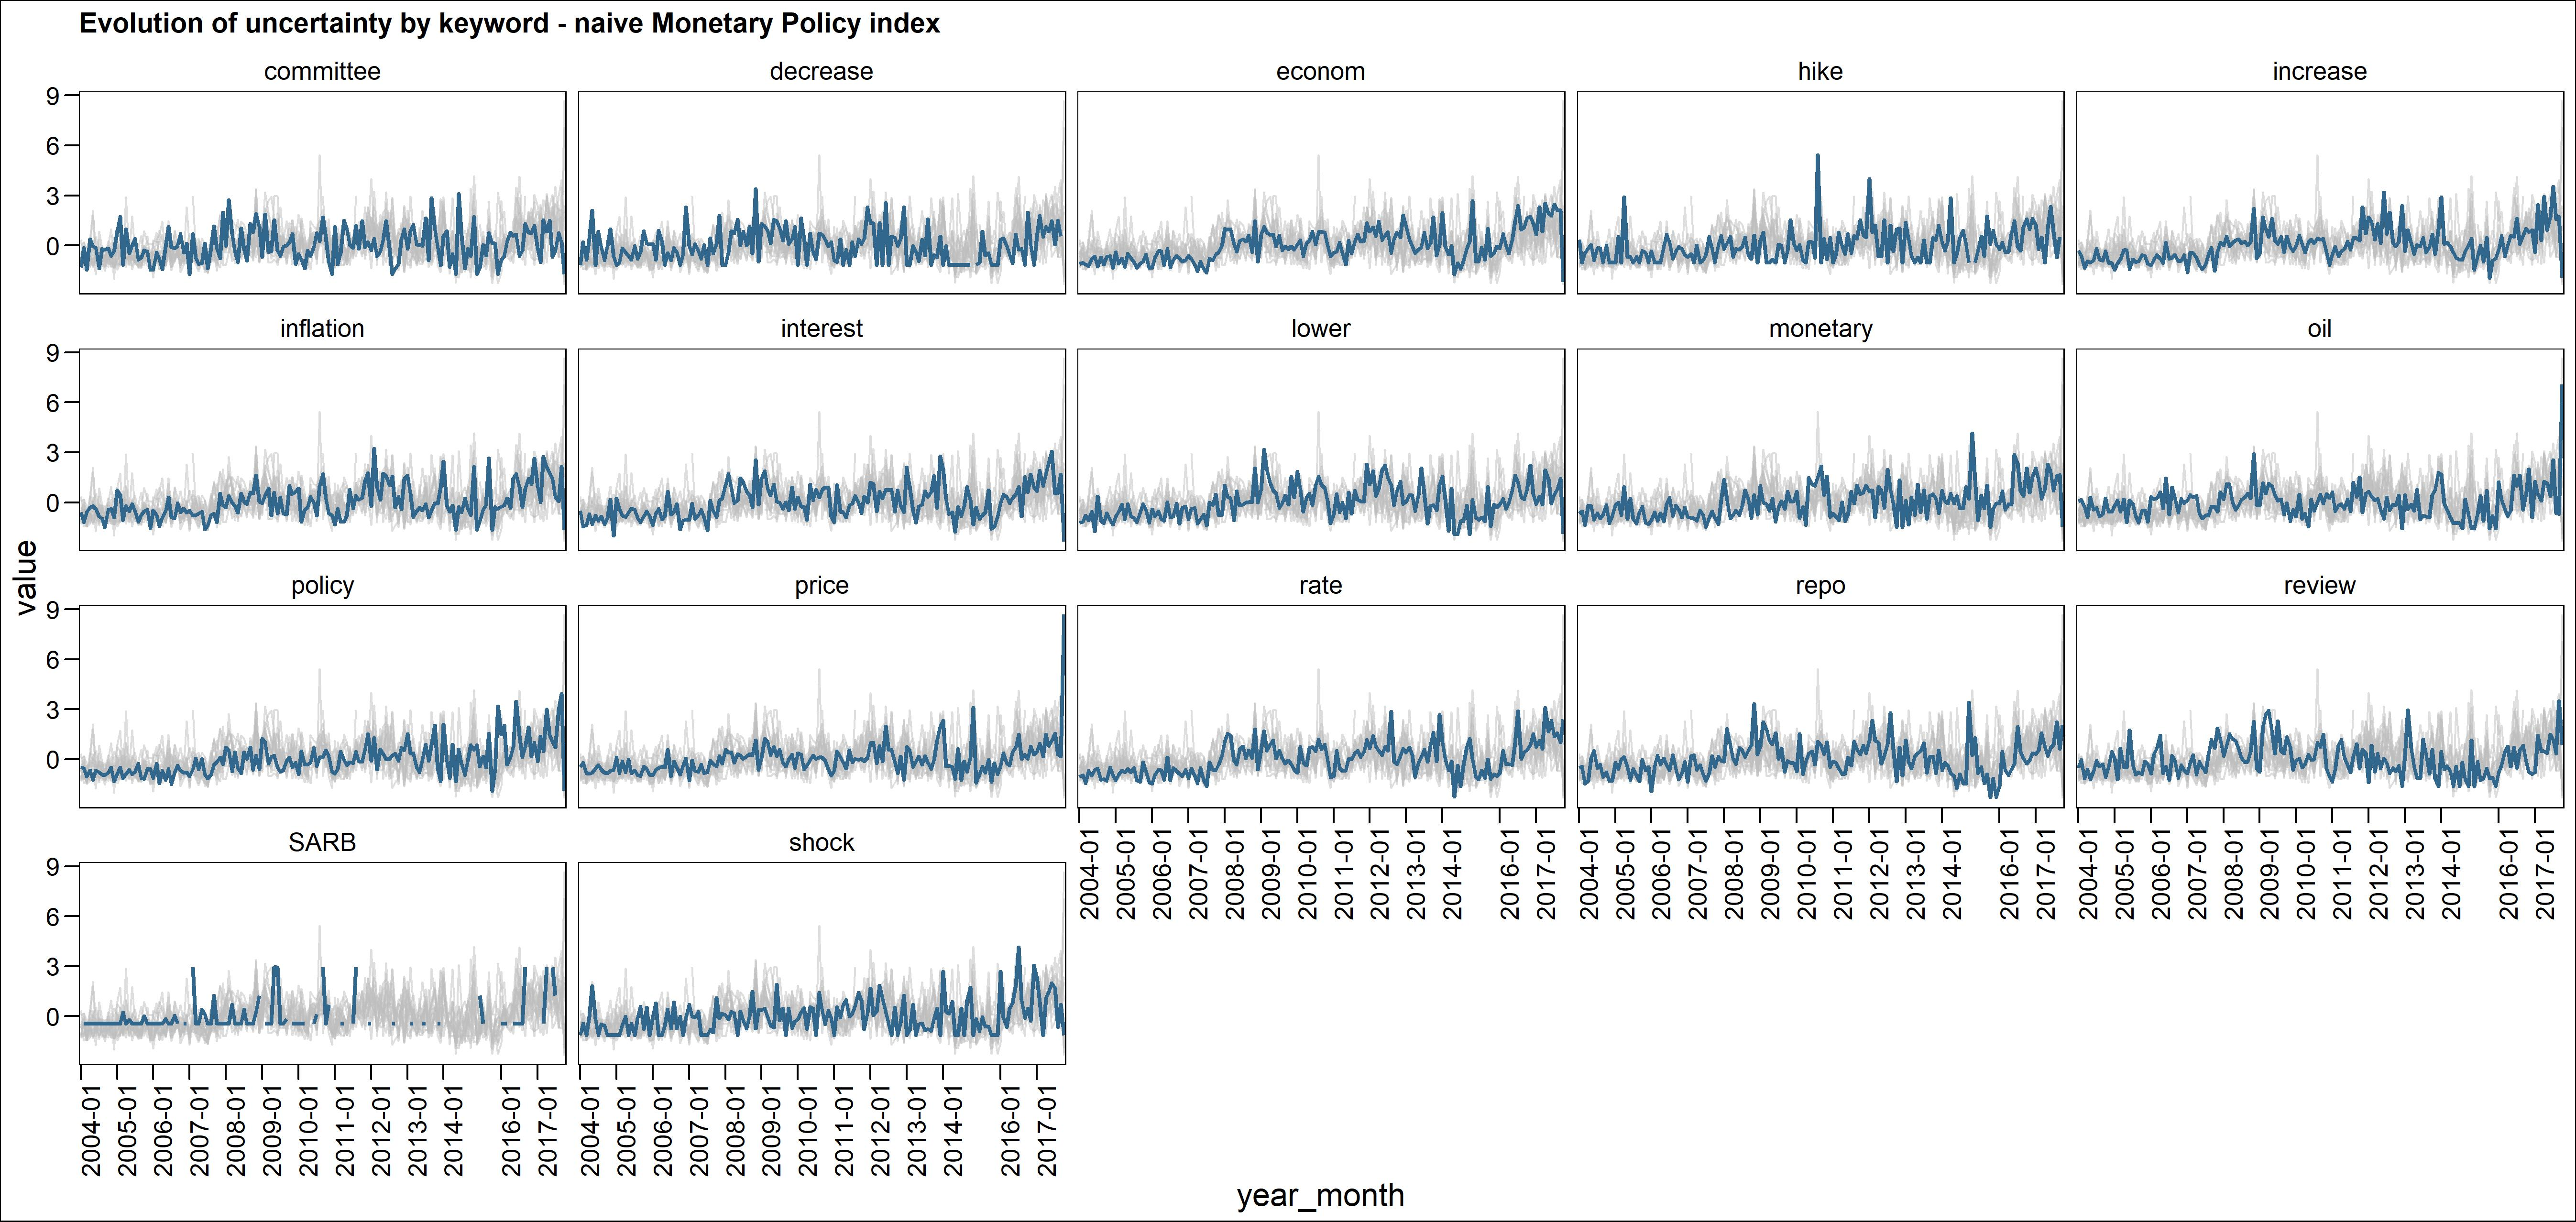
\includegraphics[width=\linewidth, keepaspectratio]{bin/monetary_key_naive}\\
	
	\caption{Composite Monetary Policy uncertainty naive index. \label{fig_mon_key_n}}
\end{figure}

\begin{figure}
	\centering
	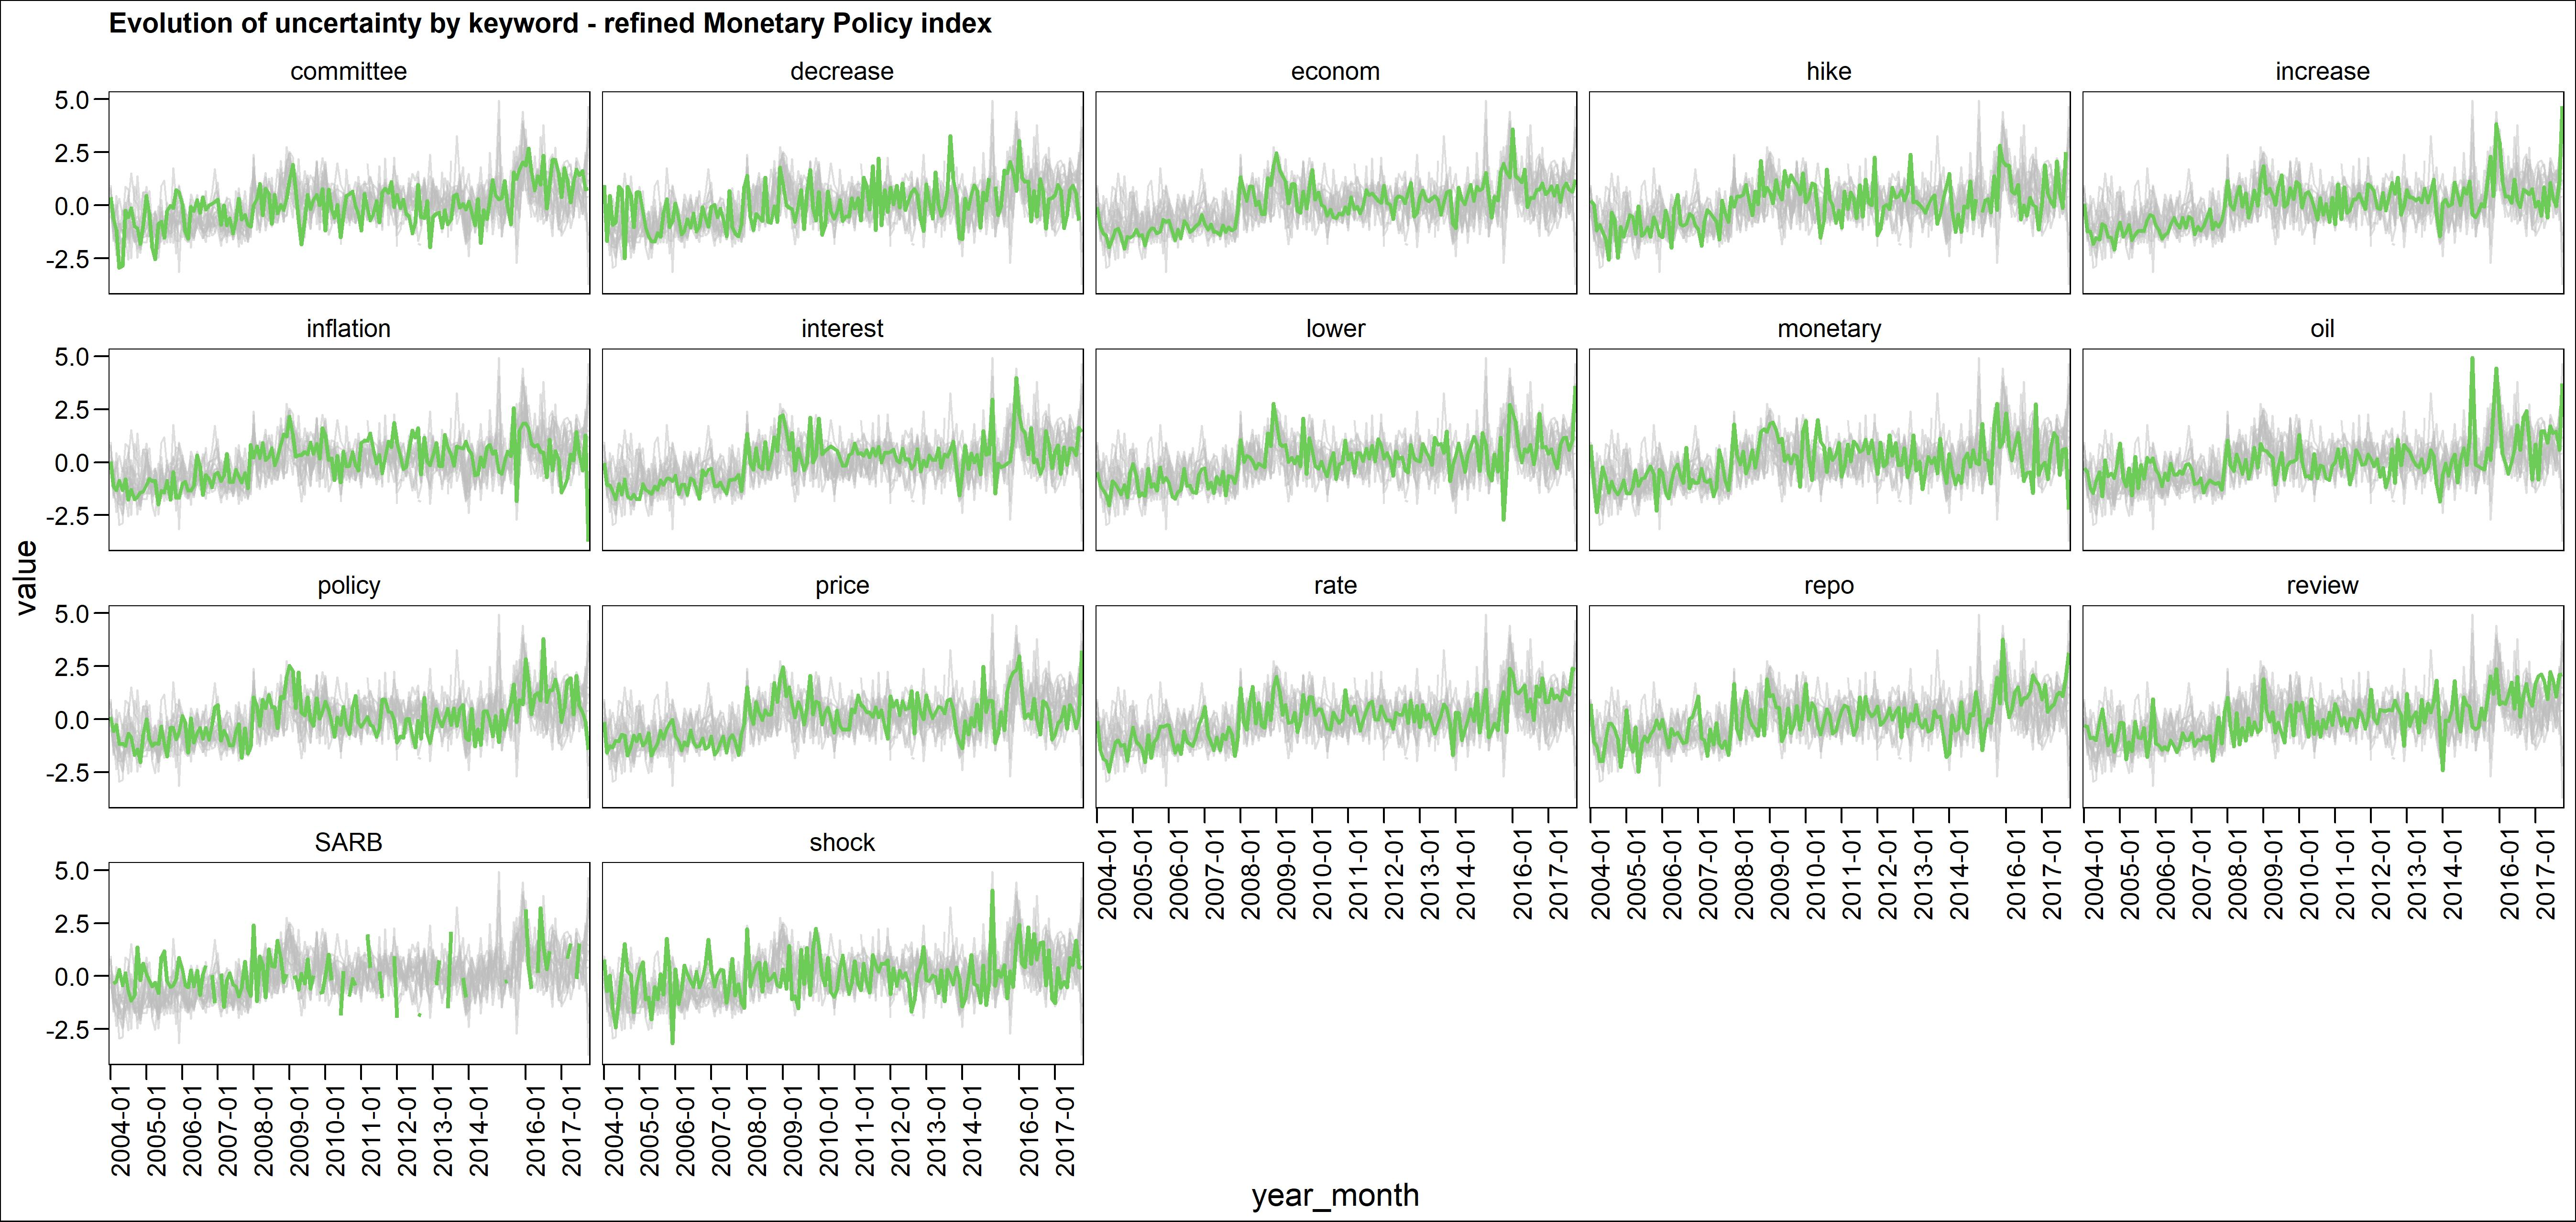
\includegraphics[width=\linewidth, keepaspectratio]{bin/monetary_key_refine}\\
	
	\caption{Composite Monetary Policy uncertainty refined index. \label{fig_mon_key_r}}
\end{figure}

\begin{figure}
	\centering
	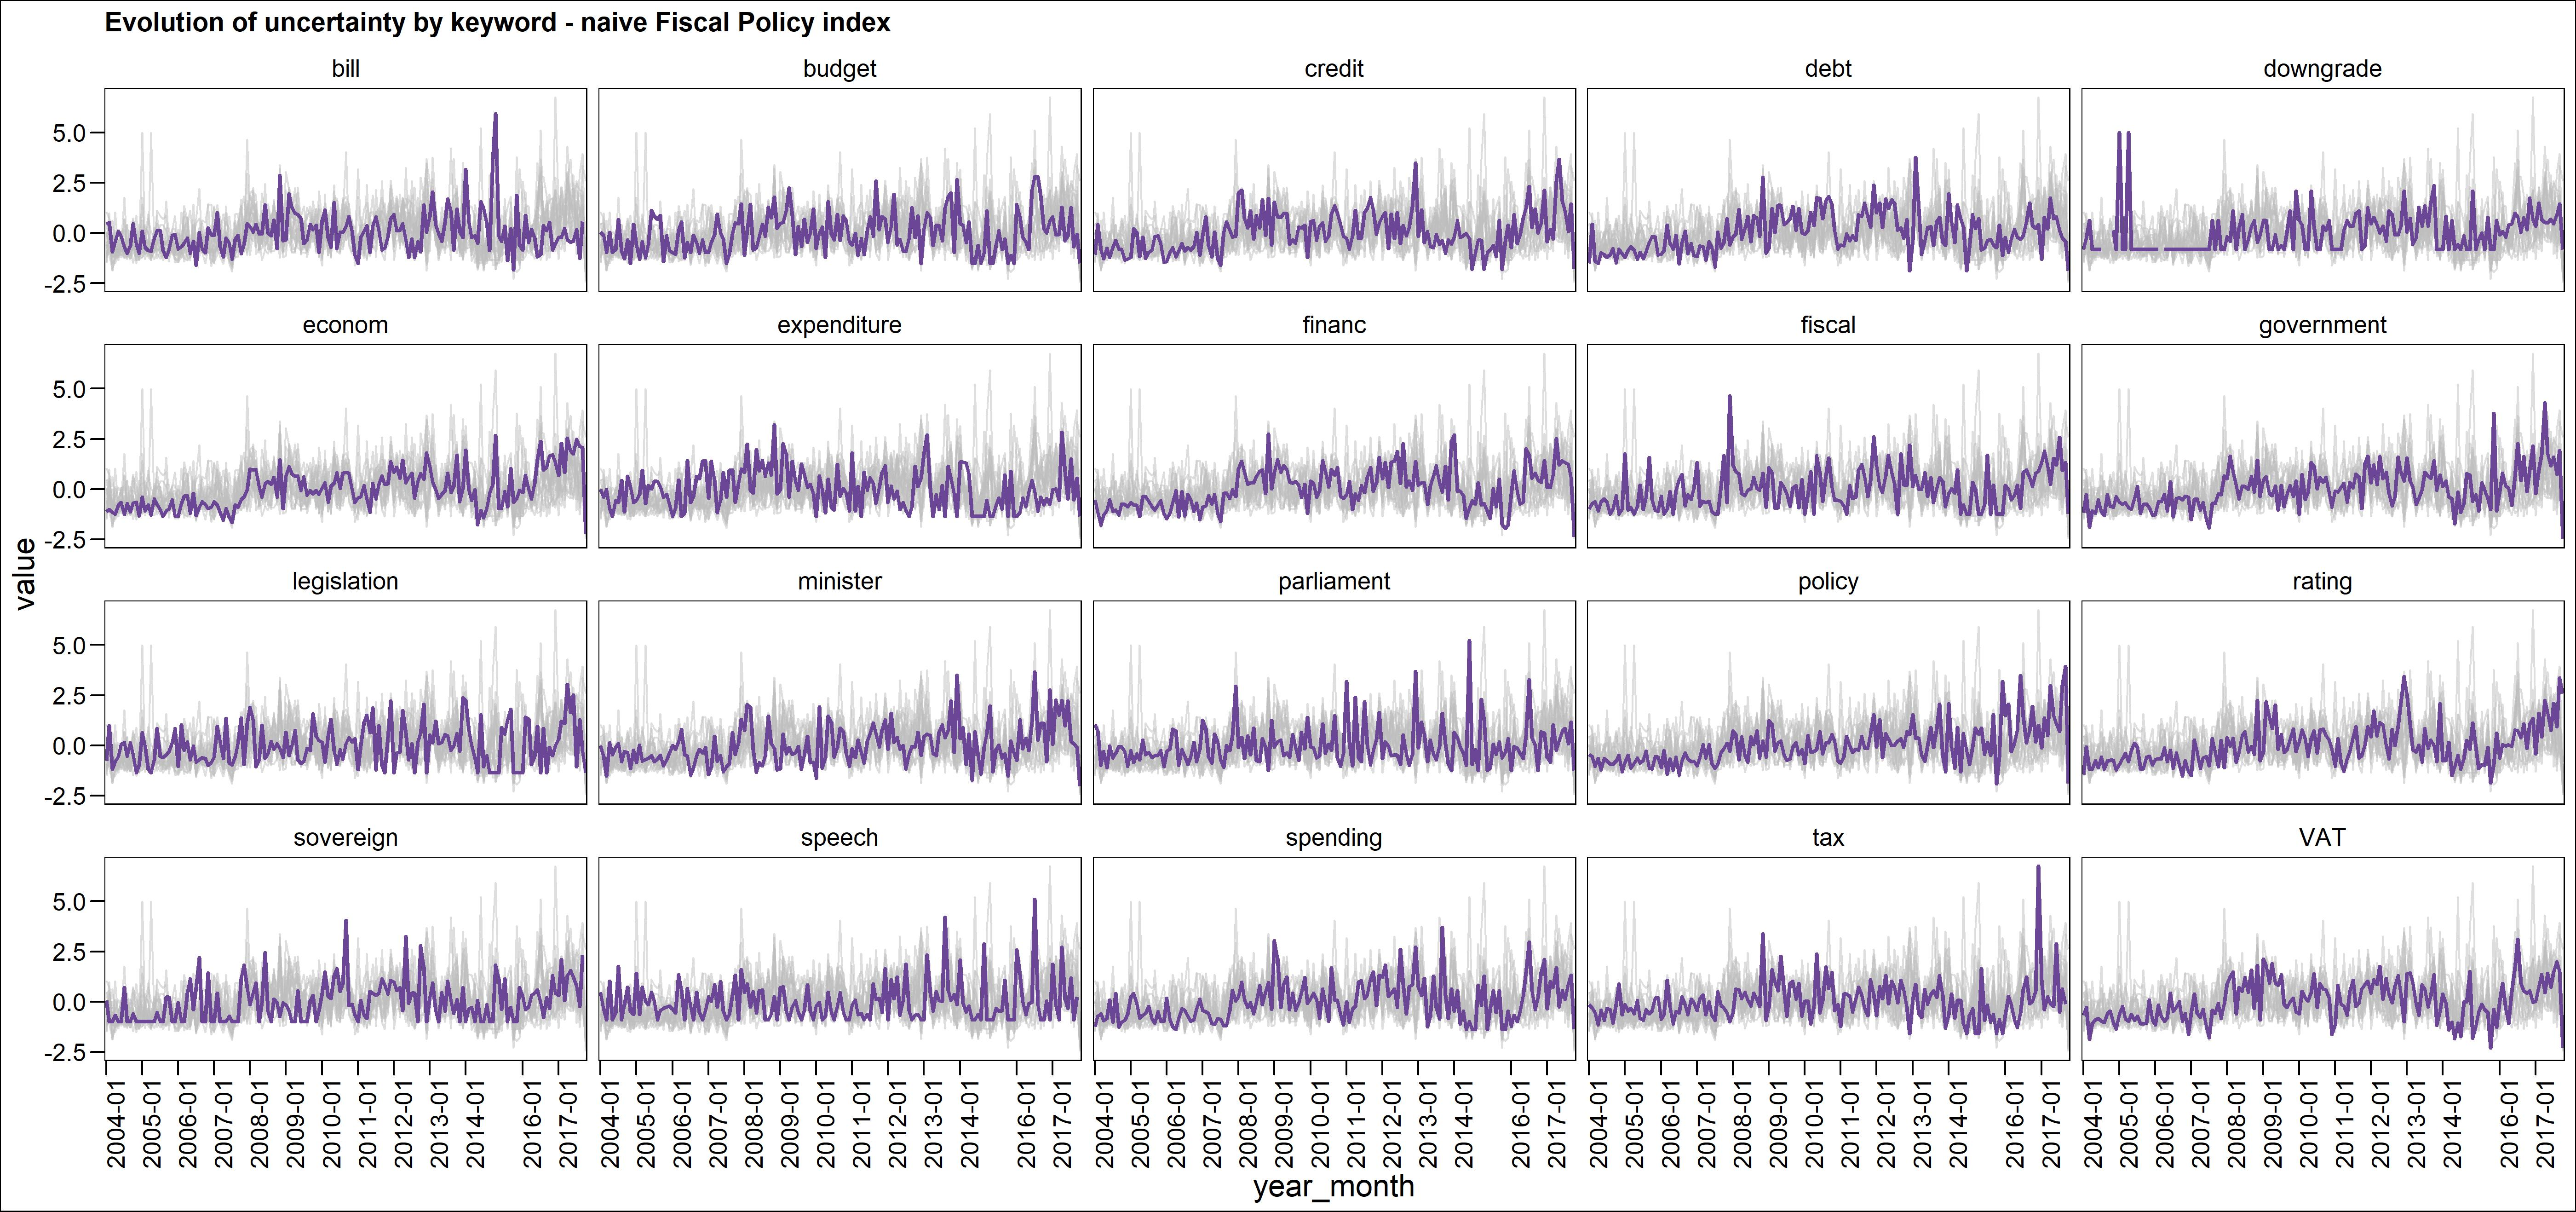
\includegraphics[width=\linewidth, keepaspectratio]{bin/fiscal_key_naive}\\
	
	\caption{Composite Fiscal Policy uncertainty naive index. \label{fig_fis_key_n}}
\end{figure}

\begin{figure}
	\centering
	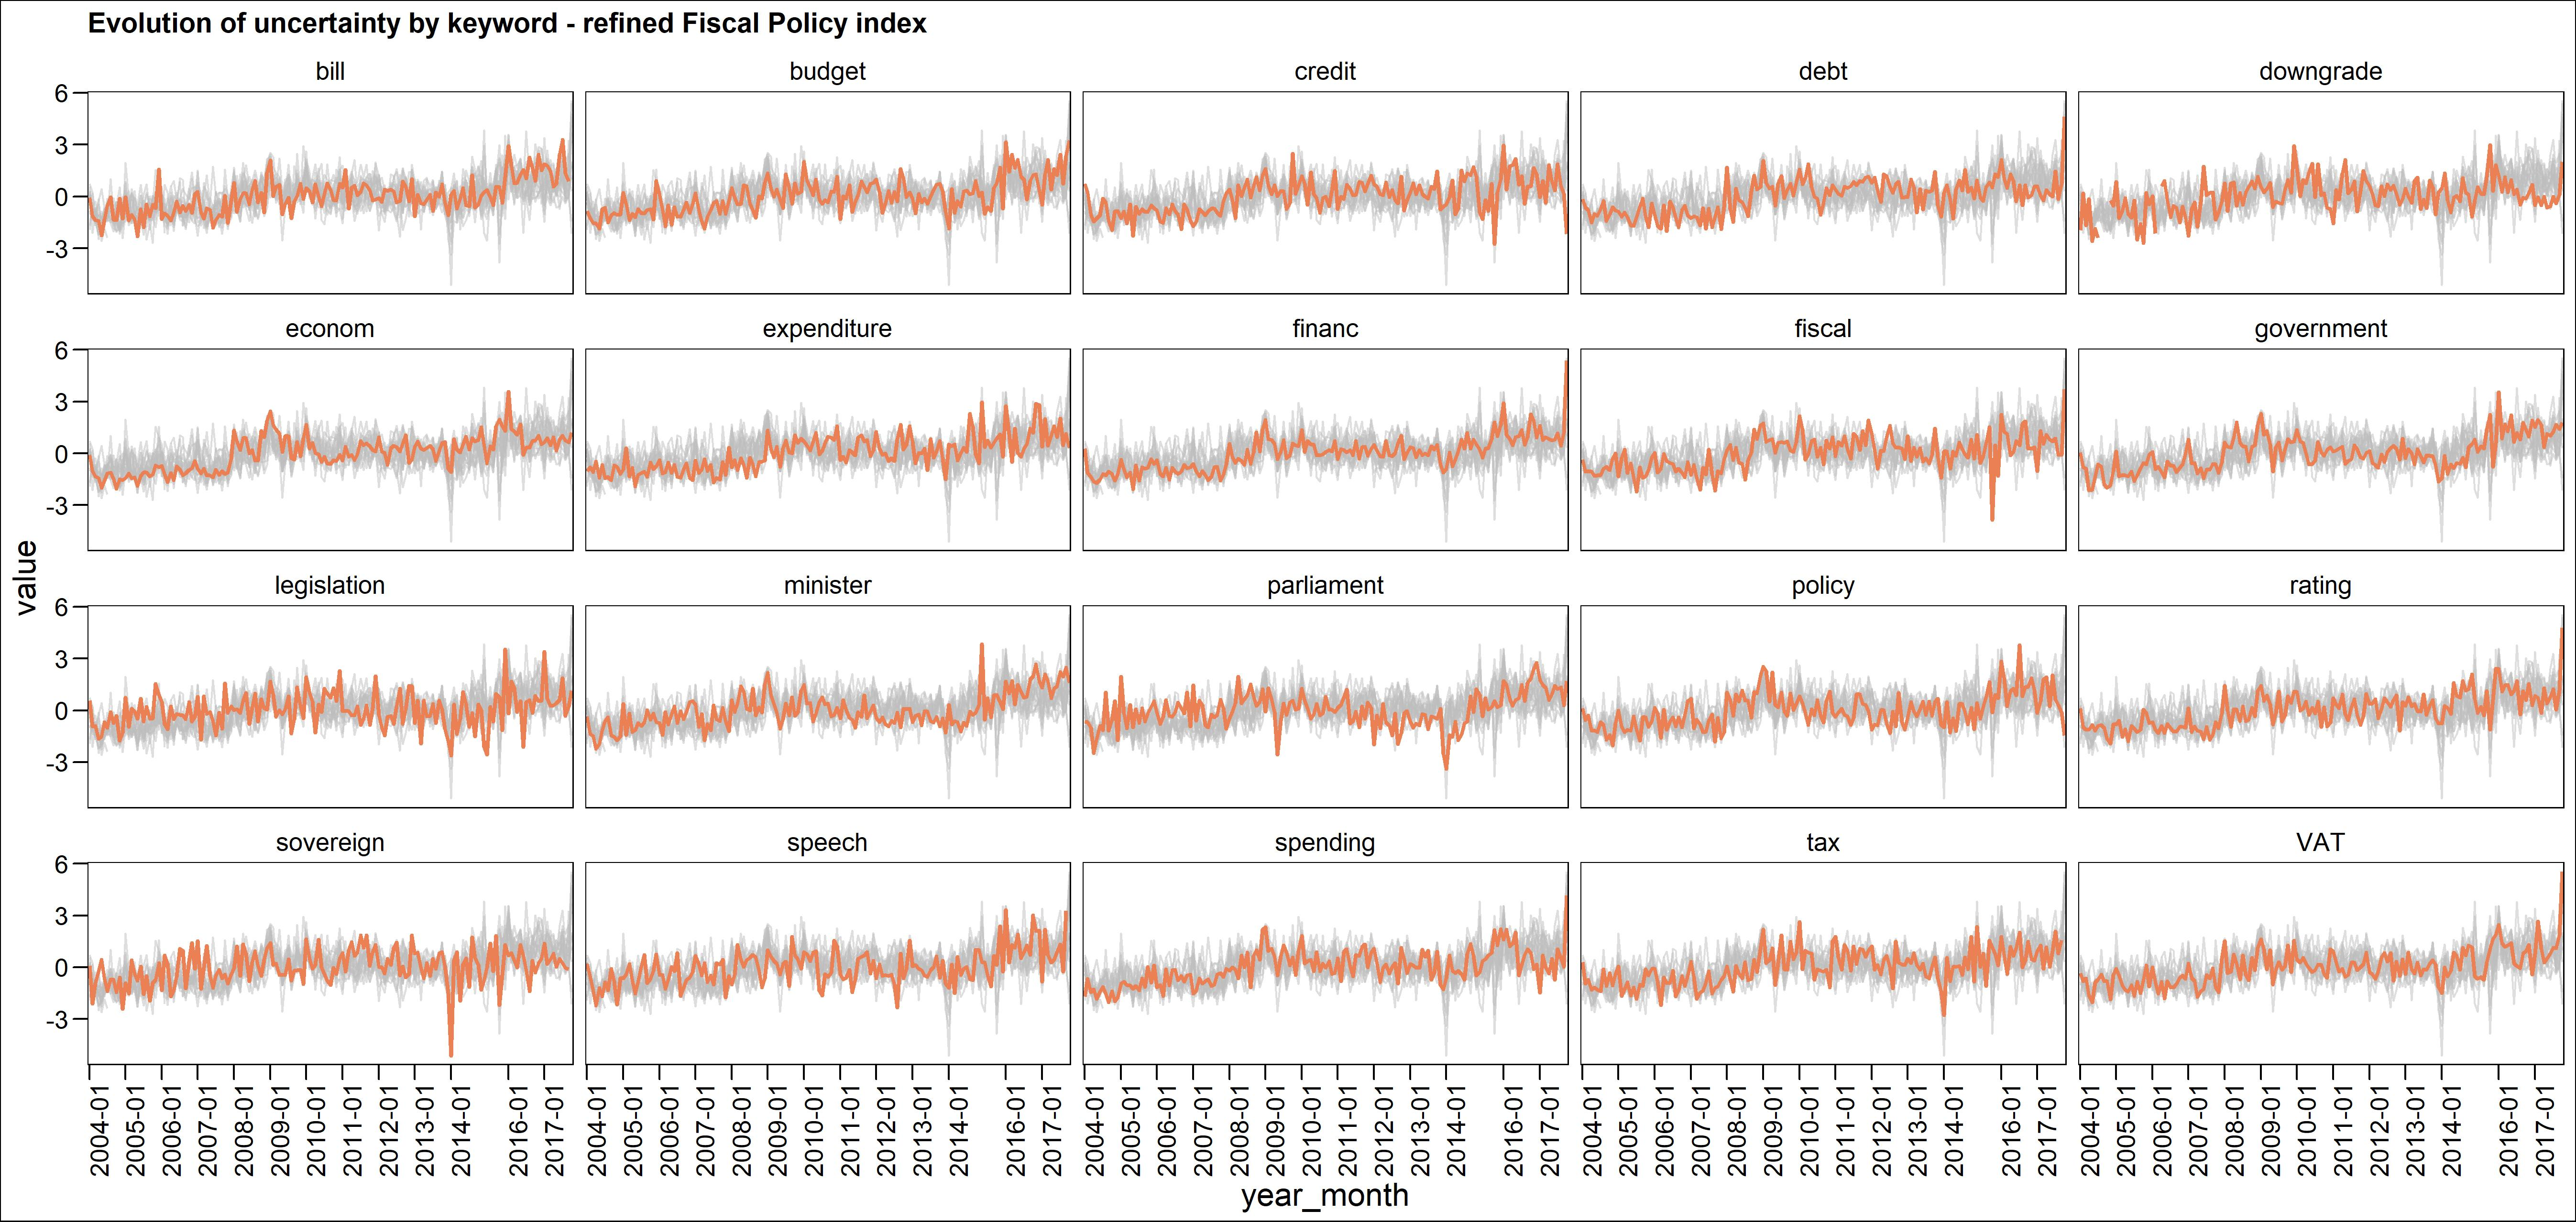
\includegraphics[width=\linewidth, keepaspectratio]{bin/fiscal_key_refine}\\
	
	\caption{Composite Fiscal Policy uncertainty refined index. \label{fig_fis_key_r}}
\end{figure}

\begin{figure}
	\centering
	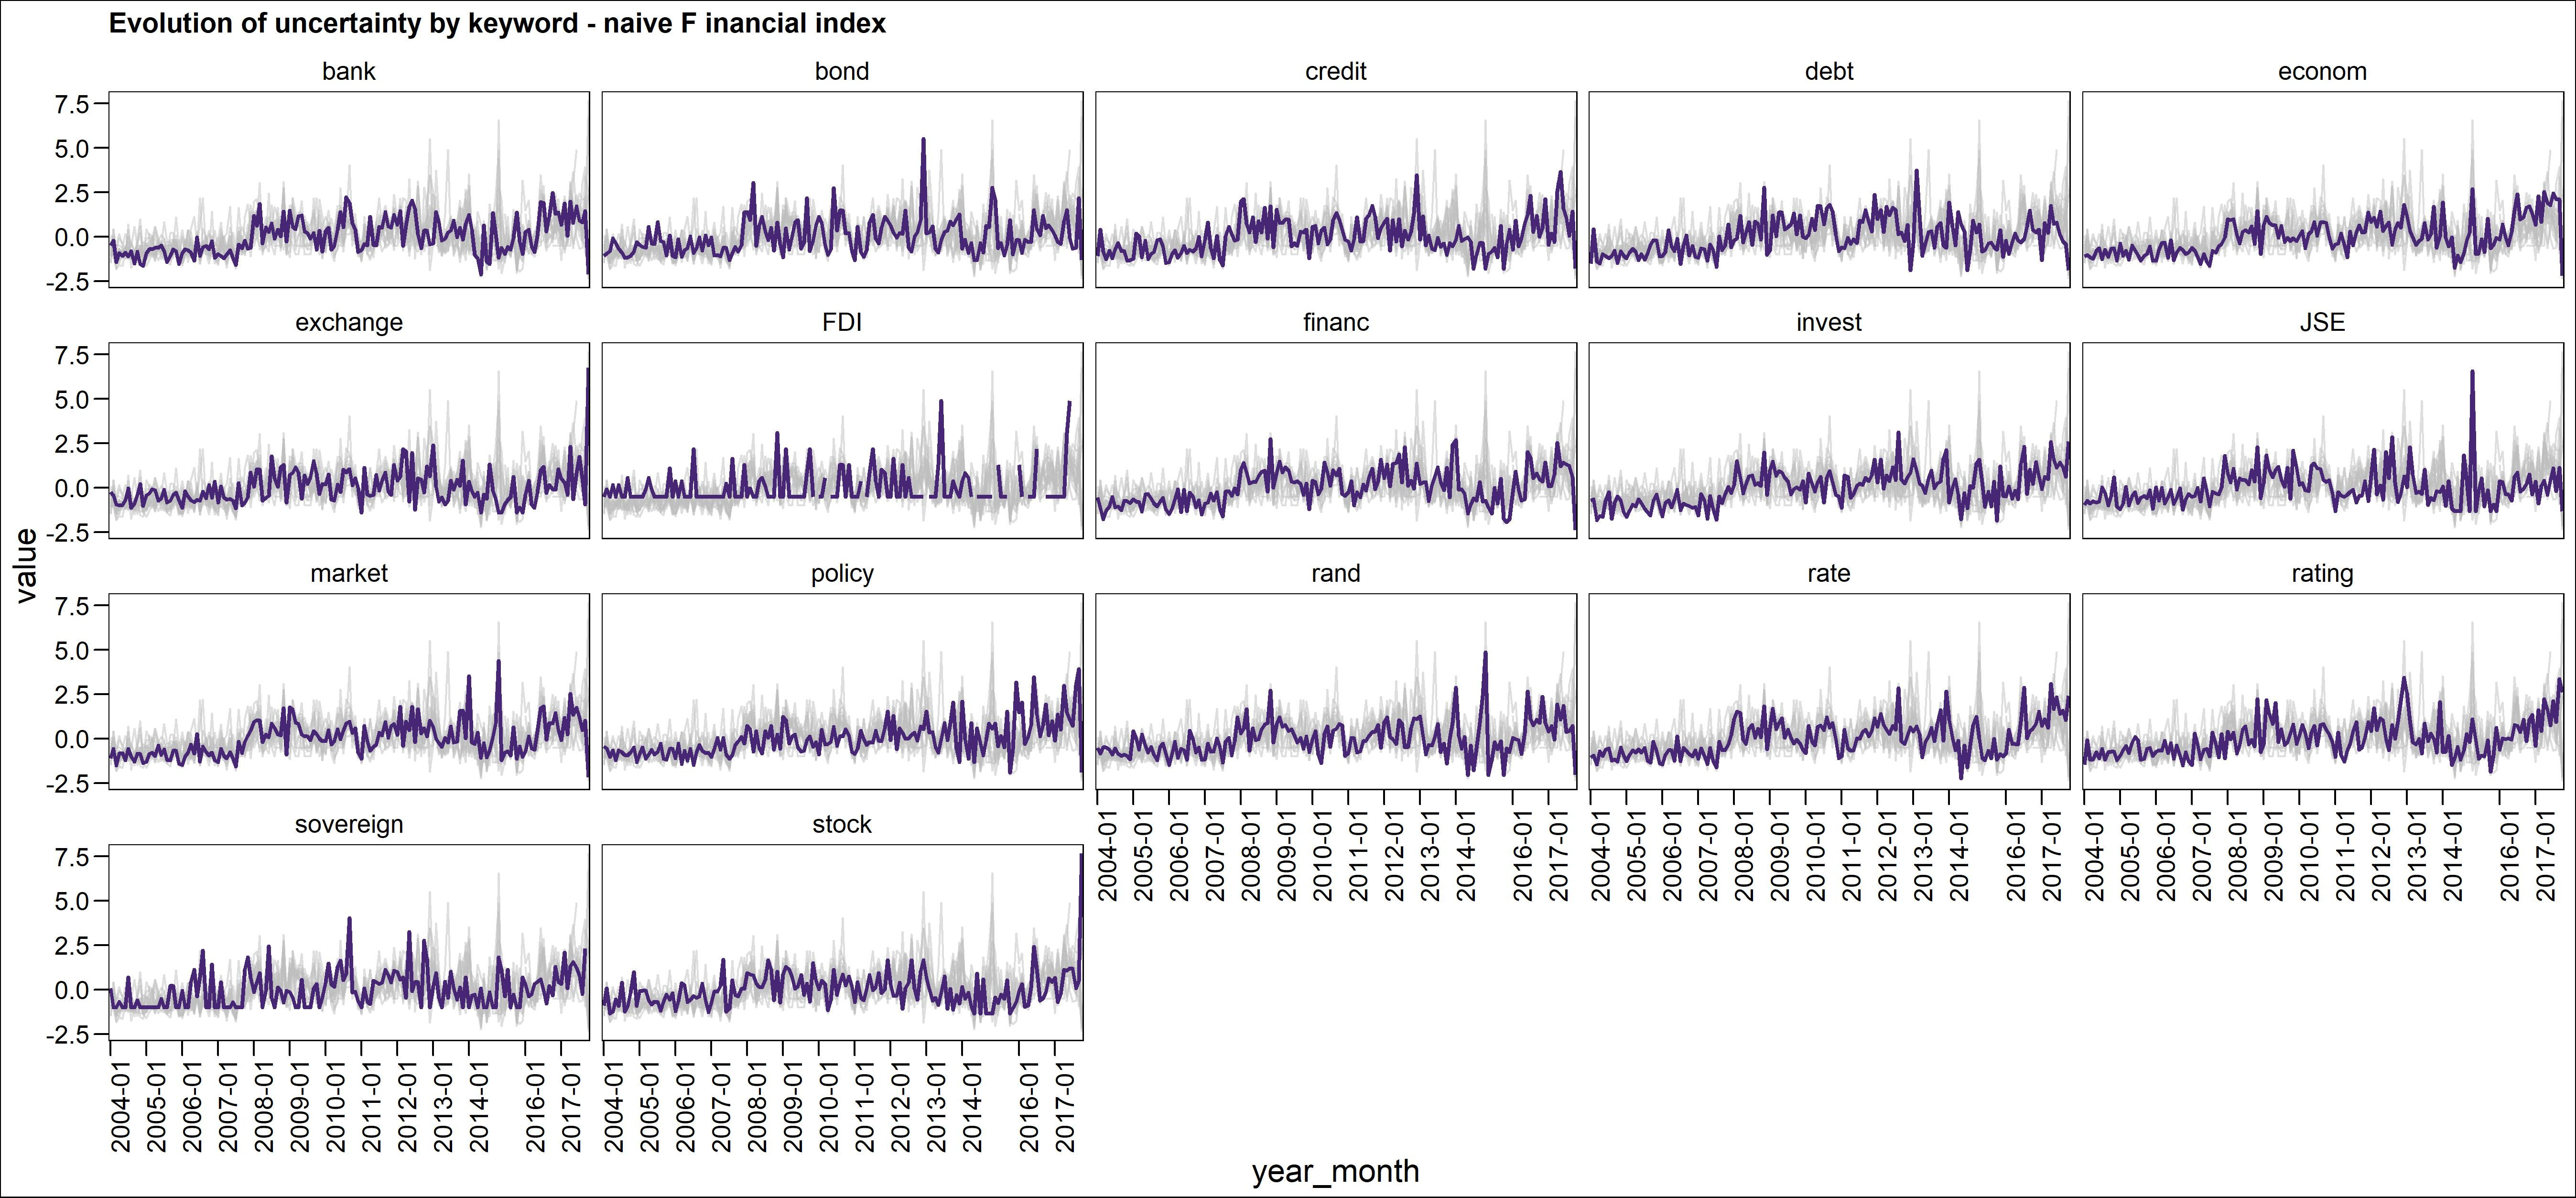
\includegraphics[width=\linewidth, keepaspectratio]{bin/financial_key_naive}\\
	
	\caption{Composite Financial market uncertainty naive index. \label{fig_fin_key_n}}
\end{figure}

\begin{figure}
	\centering
	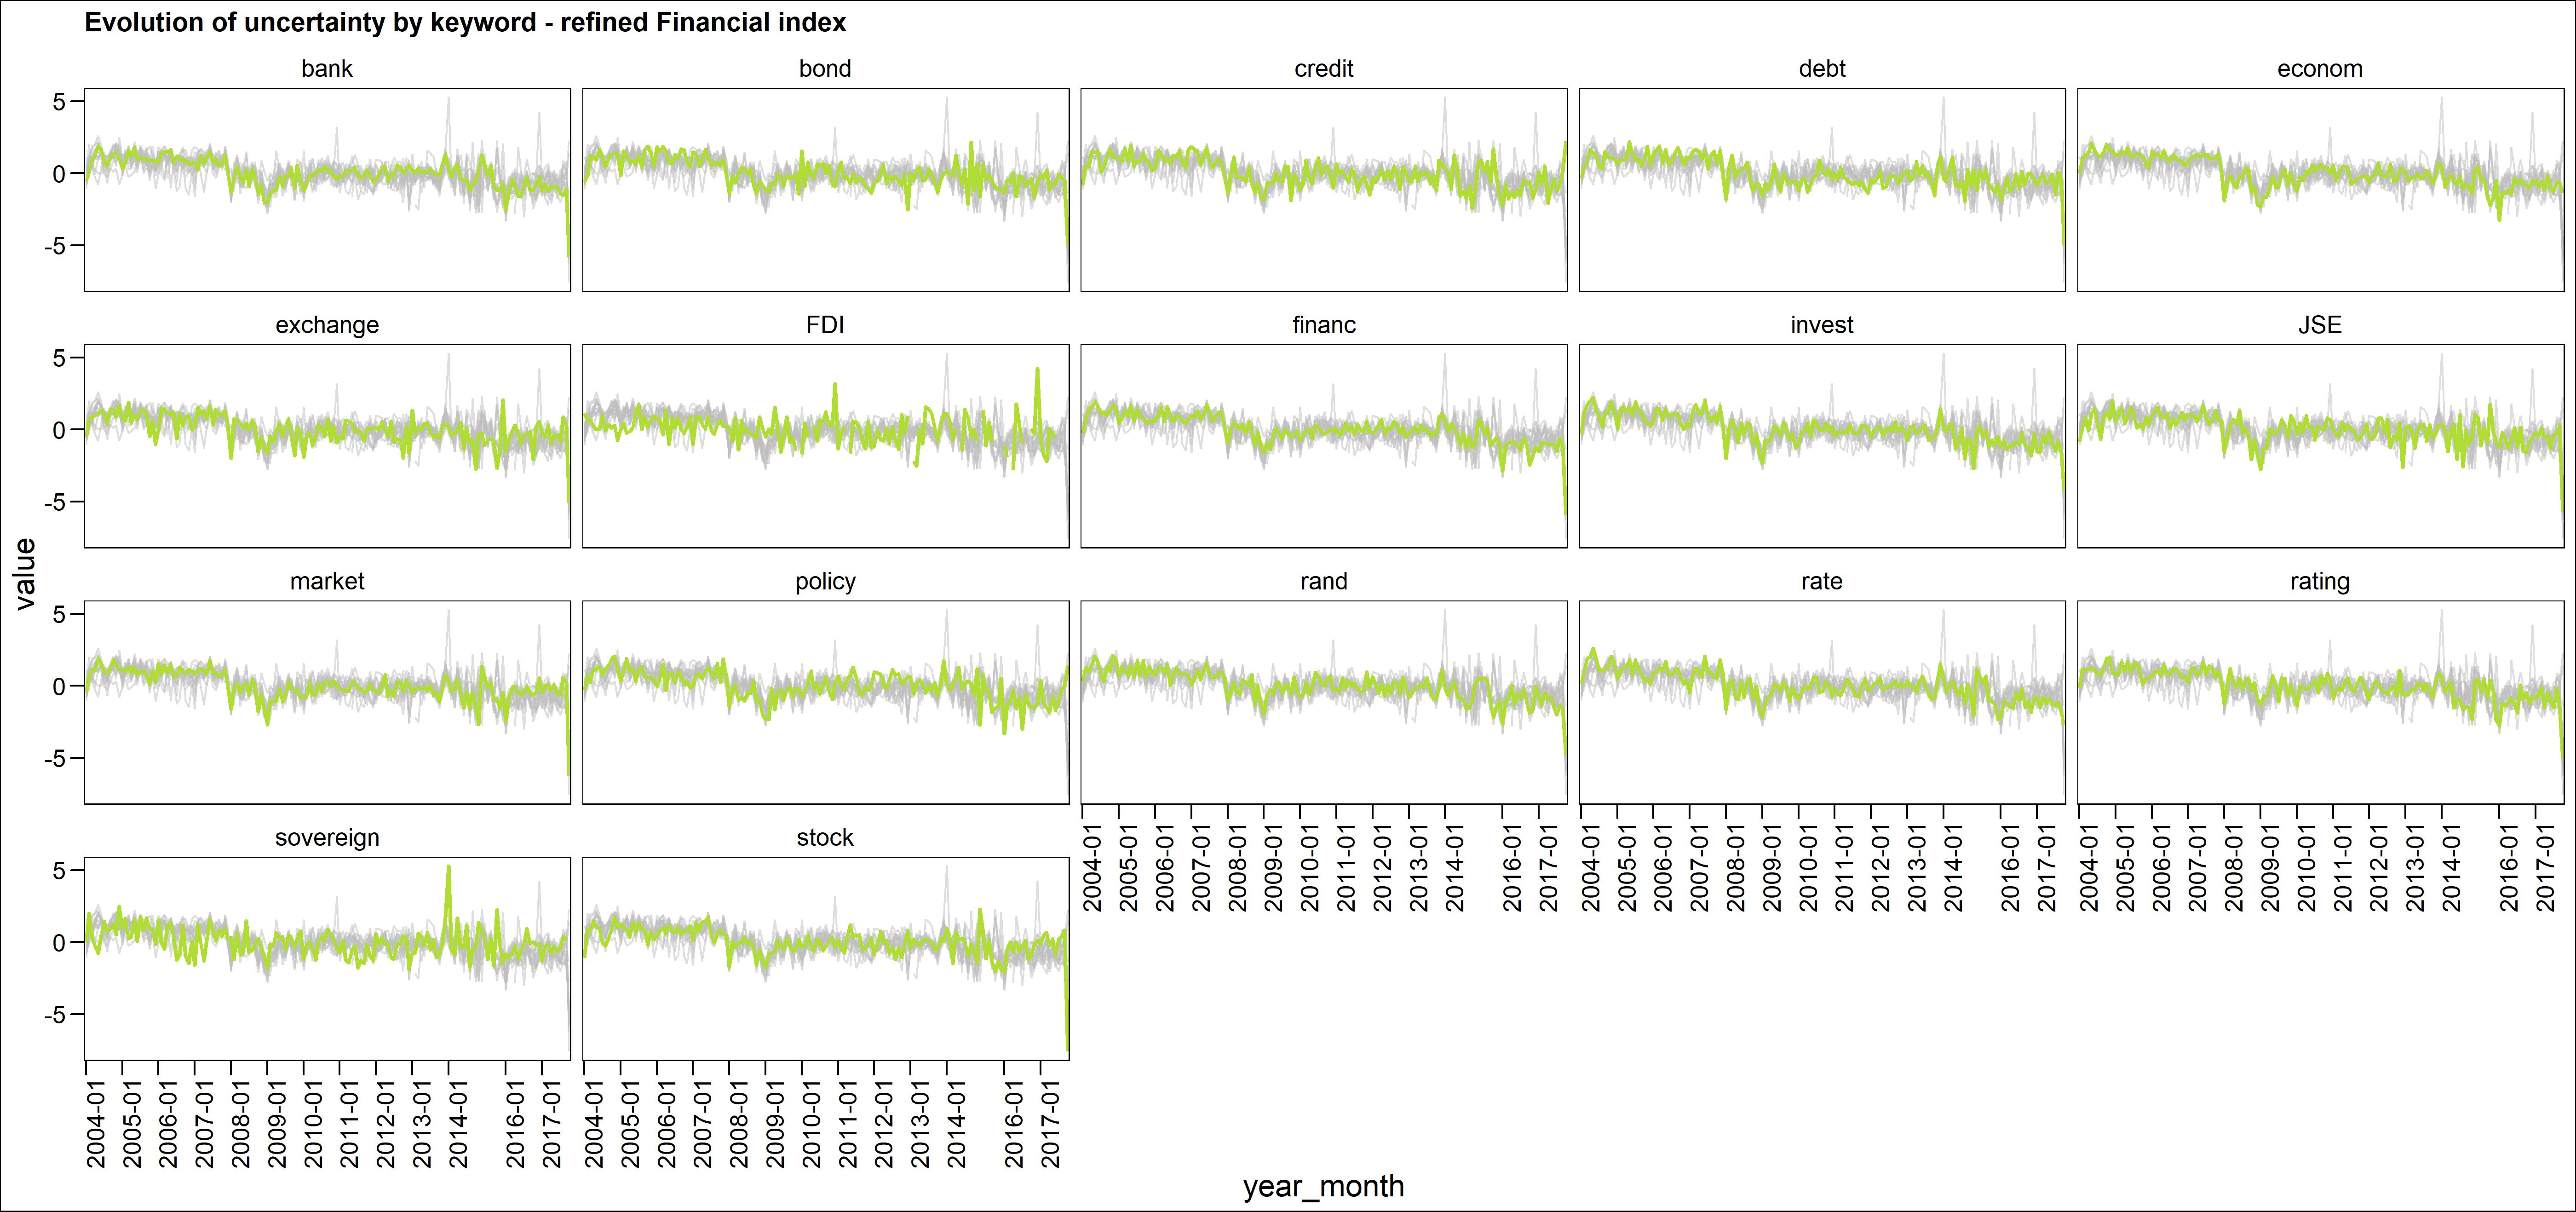
\includegraphics[width=\linewidth, keepaspectratio]{bin/financial_key_refine}\\
	
	\caption{Composite Financial market uncertainty refined index. \label{fig_fin_key_r}}
\end{figure}

\begin{figure}
	\centering
	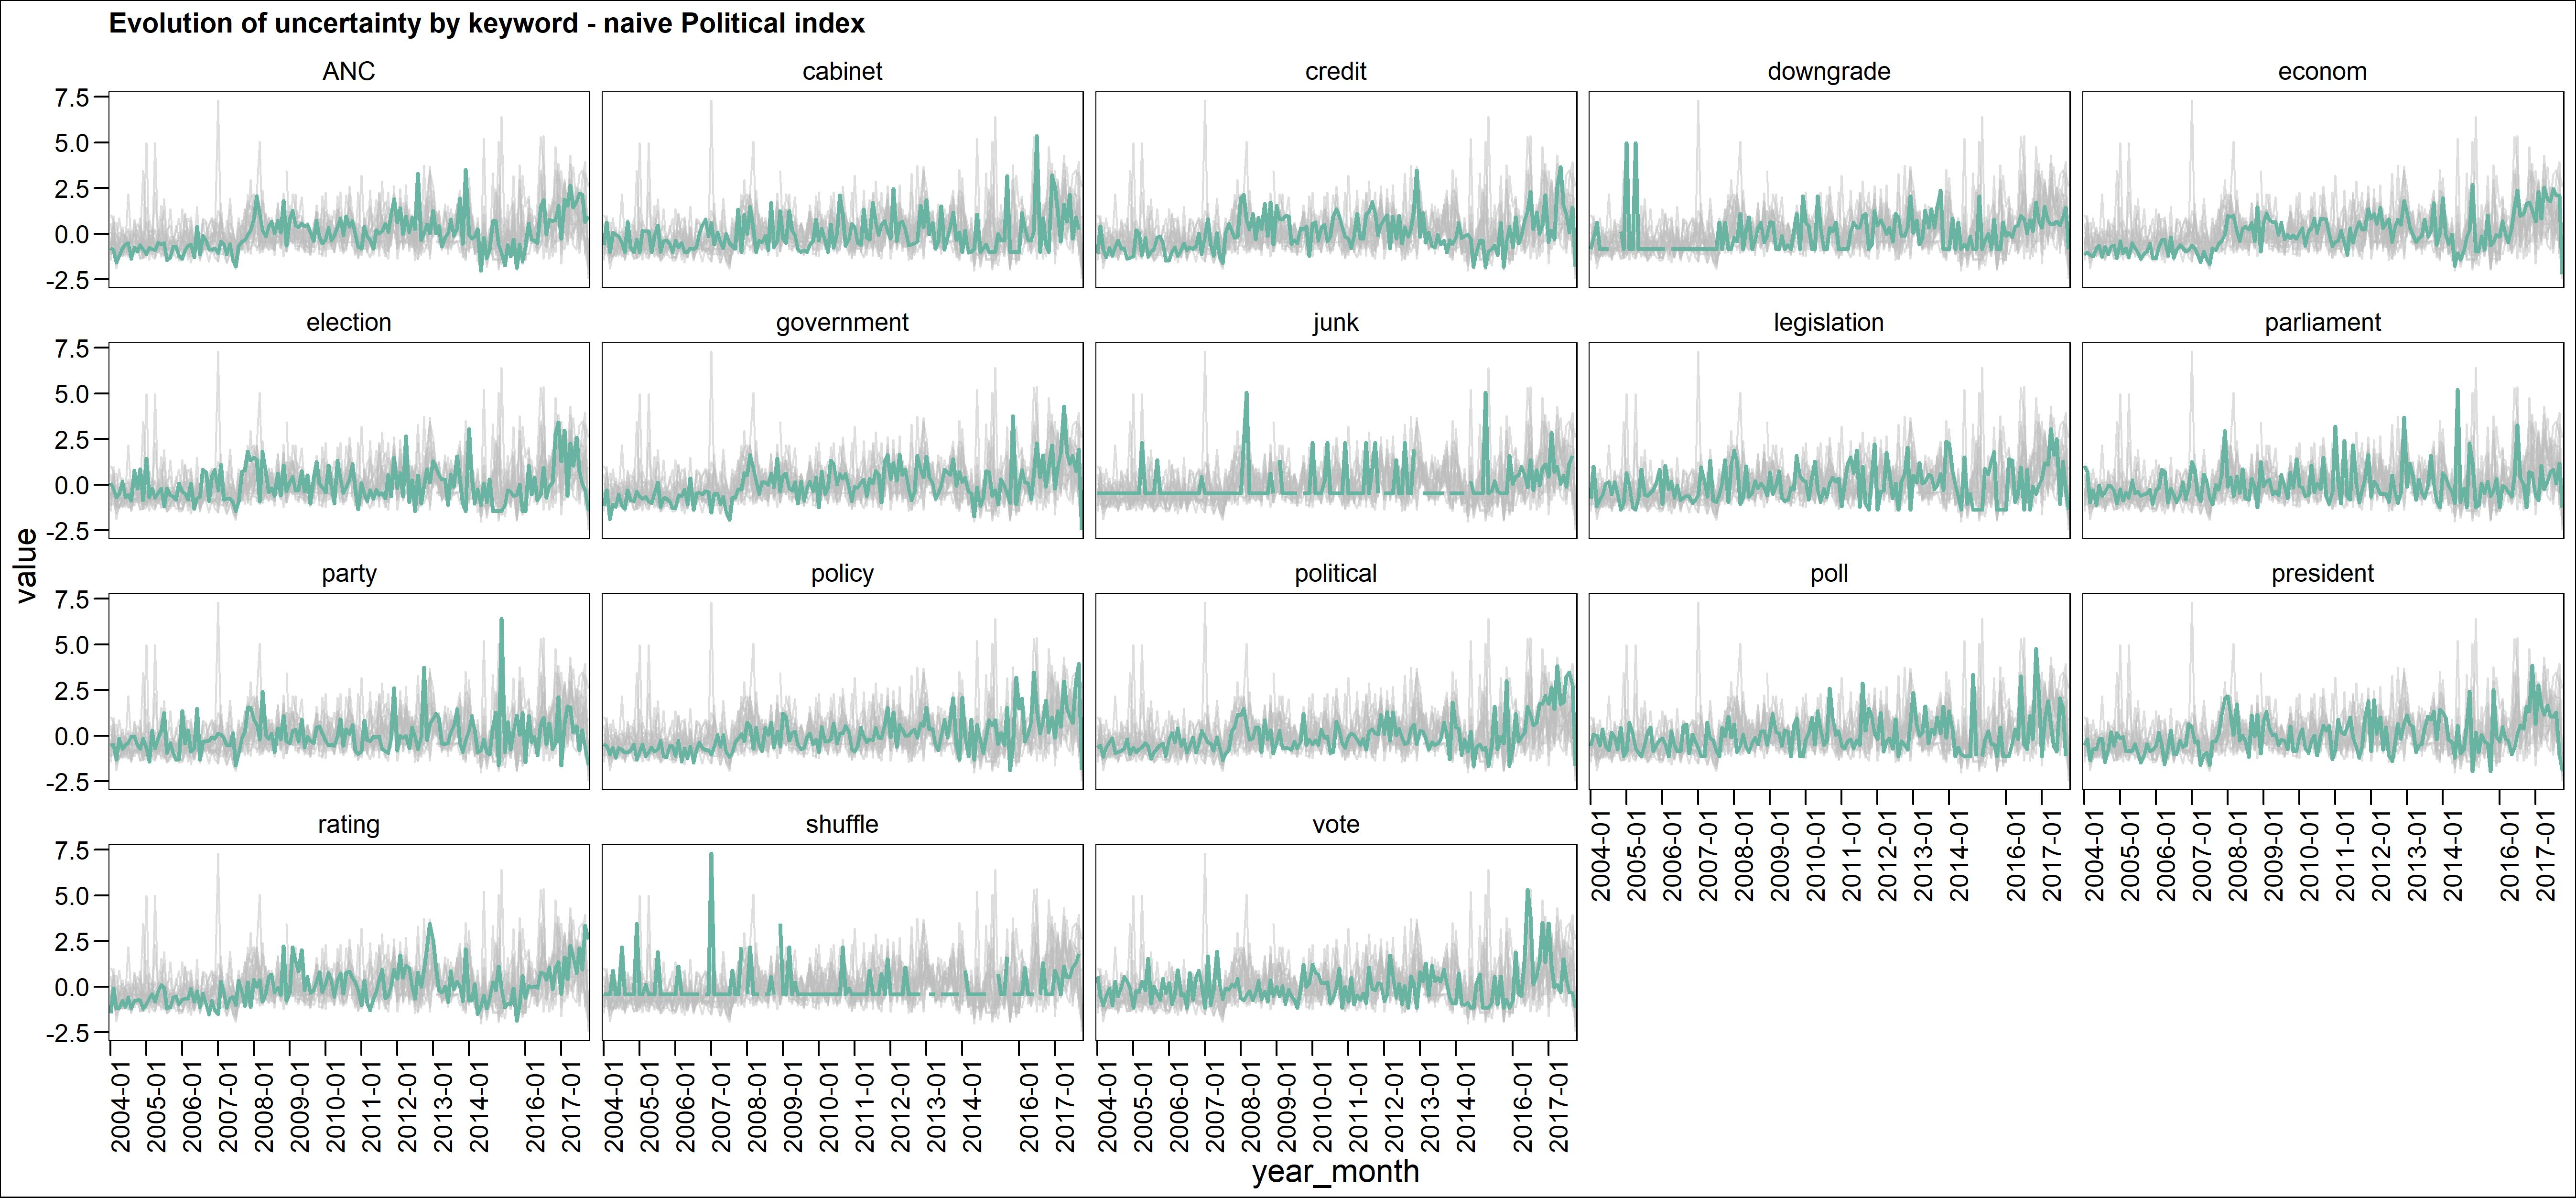
\includegraphics[width=\linewidth, keepaspectratio]{bin/pol_key_naive}\\
	
	\caption{Composite Political uncertainty naive index. \label{fig_pol_key_n}}
\end{figure}

\begin{figure}
	\centering
	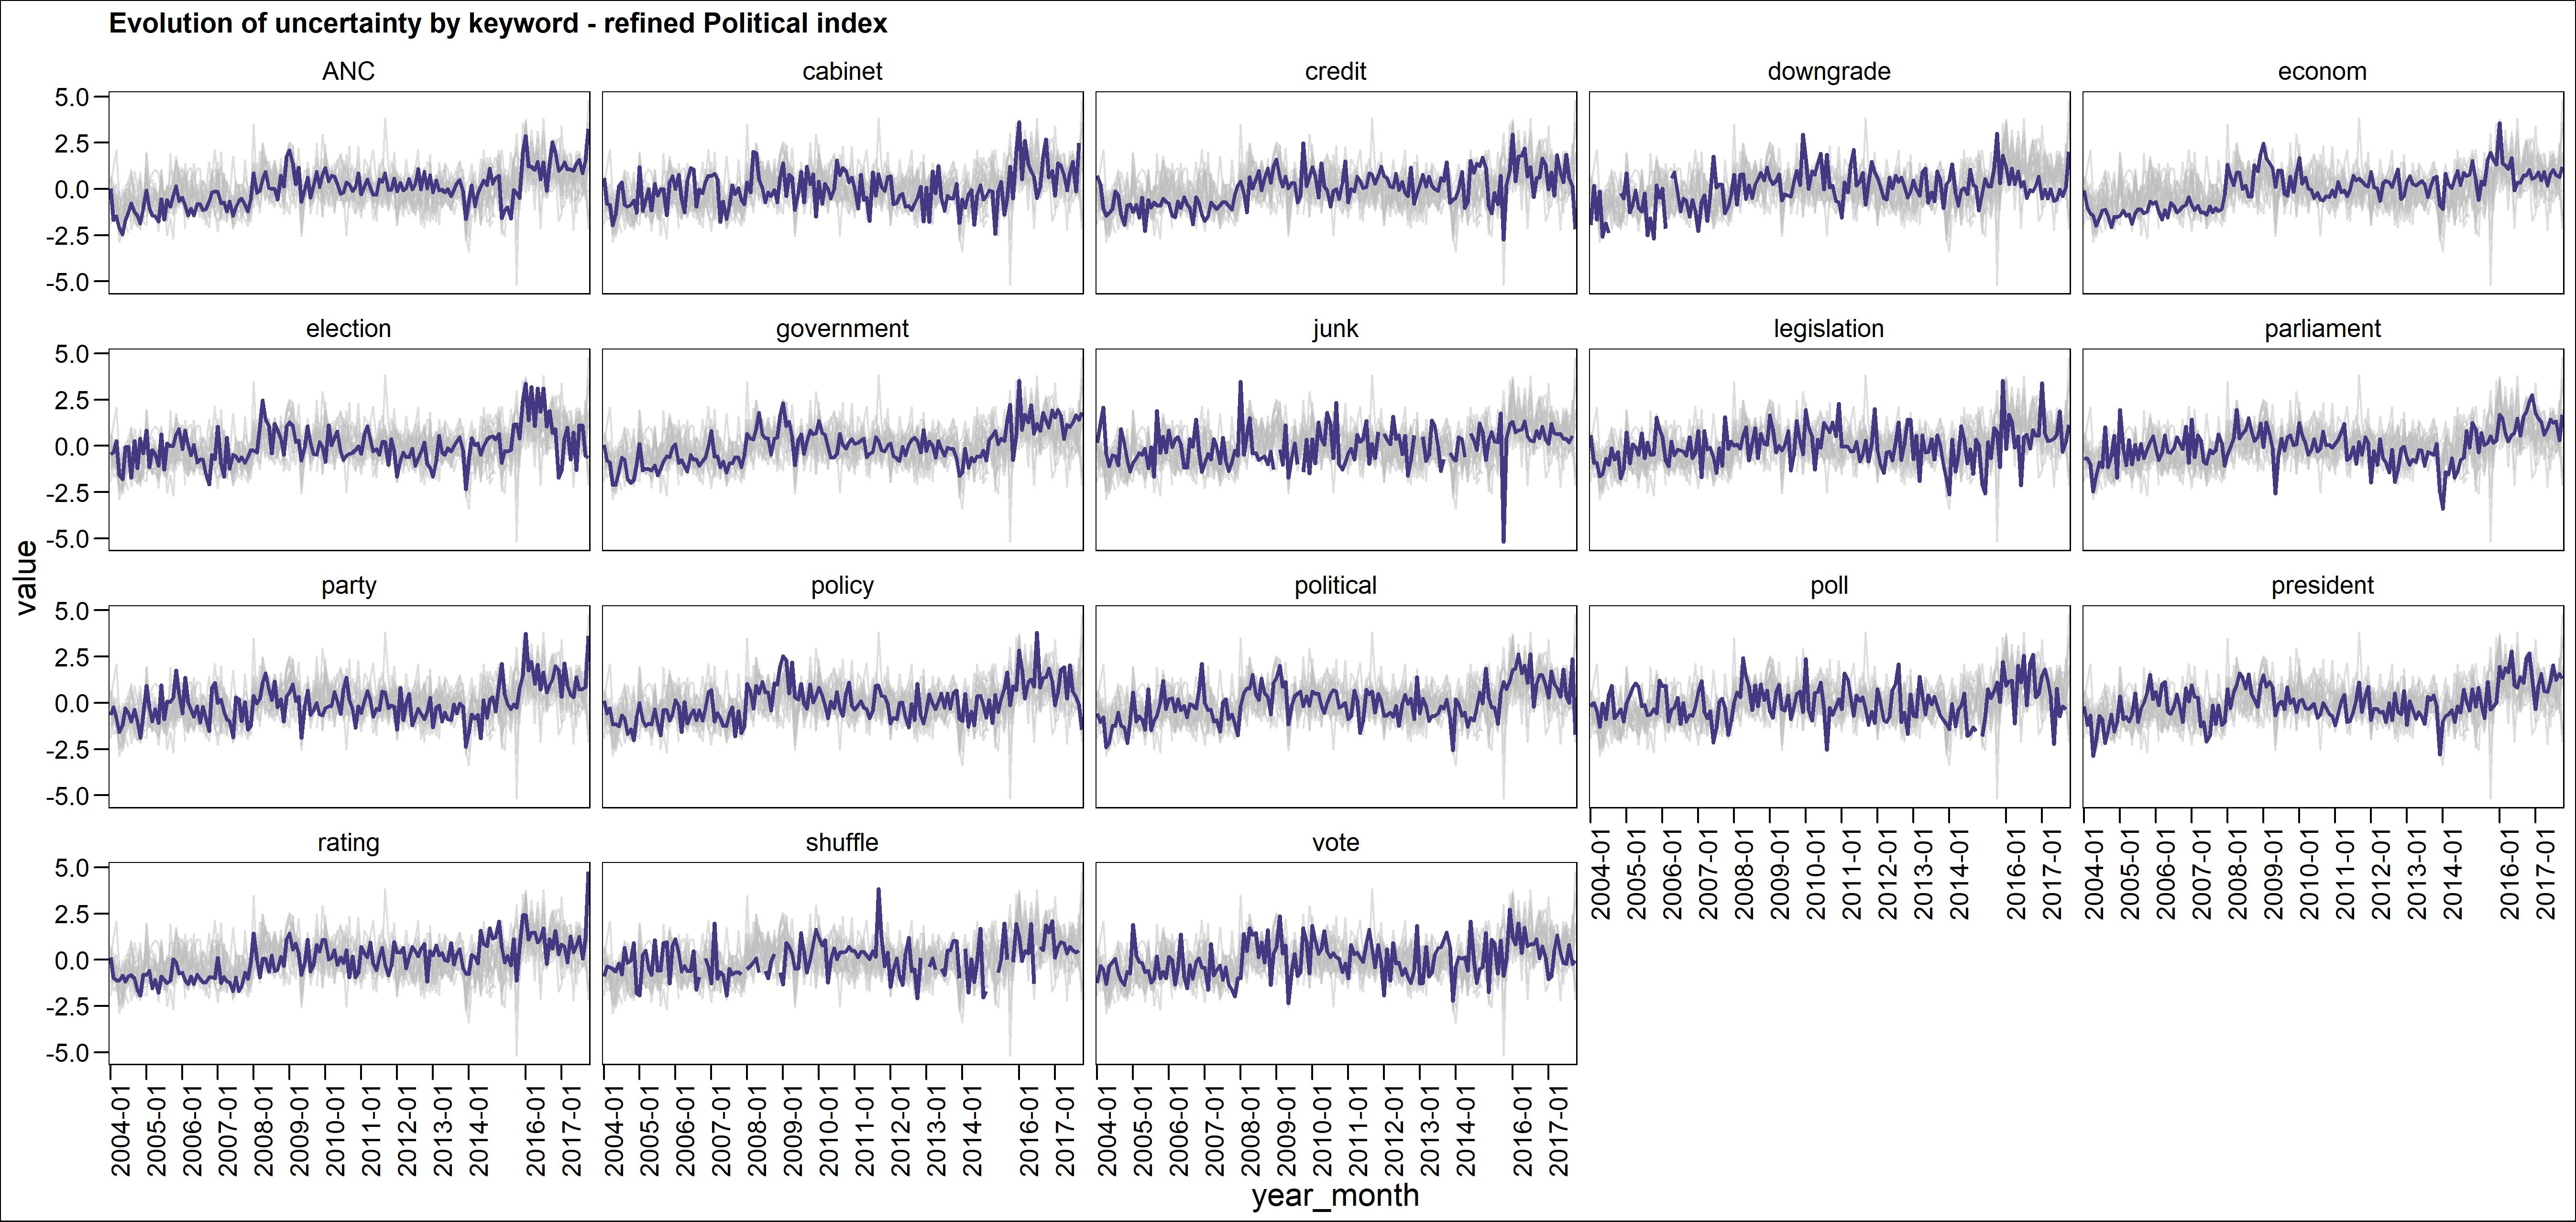
\includegraphics[width=\linewidth, keepaspectratio]{bin/pol_key_refine}\\
	\caption{Composite Political uncertainty refined index. \label{fig_pol_key_r}}
\end{figure}






\end{document}
